%--------------------------------------------------------------FORMATO
\documentclass[a4paper,12pt]{newsiambook}

%%%%%%%%%%%%%%%%%%%%%%%%%%%%%%%%%%%%%%%%%%%%%%%%%%%%%% CON ESTO LAS REFERENCIAS SON HIPERVINCULOS

\usepackage{hyperref}

%%%%%%%%%%%%%%%%%%%%%%%%%%%%%%%%%%%%%%%%%%%%%%%%%%%%%% INTRODUCIR PAQUETES

\usepackage[toc,page]{appendix}
\usepackage{tikz}
\usepackage{amsmath}
\usepackage{algpseudocode}
\usepackage{algorithm}
\usepackage{comment}

\usepackage{array} % para usar >{\raggedright}p{...}     % para una tabla
\usepackage{ragged2e} 

\usepackage{multicol} % para las firmas


% TABLES
\usepackage{adjustbox}    
\usepackage{setspace}



%%%%%%%%%%%%%%%% Lineas verticales algoritmo


\newcommand{\algruledefaultfactor}{.75}
\newcommand{\algstrut}[1][\algruledefaultfactor]{\vrule width 0pt
depth .25\baselineskip height #1\baselineskip\relax}
\newcommand*{\algrule}[1][\algorithmicindent]{\hspace*{0.5em}\vrule\algstrut
\hspace*{\dimexpr#1+0.01em}}%aumenta disminuye distancia horizontal indexado for



\makeatletter
\newcount\ALG@printindent@tempcnta
\def\ALG@printindent{%
    \ifnum \theALG@nested>0% is there anything to print
    \ifx\ALG@text\ALG@x@notext% is this an end group without any text?
    % do nothing
    \else
    \unskip
    % draw a rule for each indent level
    \ALG@printindent@tempcnta=1
    \loop
    \algrule[\csname ALG@ind@\the\ALG@printindent@tempcnta\endcsname]%
    \advance \ALG@printindent@tempcnta 1
    \ifnum \ALG@printindent@tempcnta<\numexpr\theALG@nested+1\relax% can't do <=, so add one to RHS and use < instead
    \repeat
    \fi
    \fi
}%

\patchcmd{\ALG@doentity}{\noindent\hskip\ALG@tlm}{\ALG@printindent}{}{\errmessage{failed to patch}}

\AtBeginEnvironment{algorithmic}{\lineskip0pt}

\newcommand*\Let[2]{\State #1 $\gets$ #2}
\newcommand*\Stateh{\State \algstrut[1]}
% Añade este comando para los números de línea
\newcommand{\LineNumber}[1]{\makebox[2em][r]{#1:}}


%%%%%%%%%%%%%%%%




%%%%%%%%%%%%%%%%%%%%%%%%%%%%%%%%%%%%%%%%%%%%%%%%%%%%%% PATH FOR THE IMAGES

%\graphicspath{{Images/}{Images/P1}{Images/P2}{Images/P3}{Images/P4}{Images/P5}}

%%%%%%%%%%%%%%%%%%%%%%%%%%%%%%%%%%%%%%%%%%%%%%%%%%%%%% ESTILO PROPIO DEL TEXTO

\usepackage[a4paper, total={15cm, 22cm}]{geometry}


\voffset=2cm

\renewcommand{\labelenumi}{\roman{enumi}} % bulletpoints for enumerate

\newcommand{\csch}{\makebox{csch}}
\newcommand{\sech}{\makebox{sech}}

\newcommand{\clearemptydoublepage}{\newpage{\pagestyle{empty}\cleardoublepage}}

\newcommand{\letquote}{\sffamily \small \slshape}
\newcommand{\dedica}{\sffamily \slshape}

%\newdateformat{mydate}{\bf \Large \monthname[\THEMONTH], \THEYEAR}
%\newdateformat{mydatebis}{\bf \large \monthname[\THEMONTH], \THEYEAR}

%%%%%%%%%%%%%%%%%%%%%%%%%%%%%%%%%%%%%%%%%%%%%%%%%%%%%%%% CARACTERISTICAS DEL DOCUMENTO
%\renewcommand{\baselinestretch}{1.1}                   % espaciado entre lineas
%\language=1                                            
%\baselineskip=18pt                                     % cortes
%\oddsidemargin 1.8cm
%\evensidemargin 0.5cm
\fboxsep=0.3cm
\fboxrule=2pt

\thispagestyle{empty}



%%%%%%%%%%%%%%%%%%%%%%%%%%%%%%%%%%%%%%%%%%%%%%%%%%%%%%%%%%%%%%%%% INICIO DEL DOCUMENTO
\makeindex                                                       % indice



%\addbibresource{ref_thesis.bib}




%%%%%%%%%%%%%%%%%%%%%%%%



\begin{document}




%%%%%%%%% margin equal of odd and even

%\setlength{\evensidemargin}{0cm}
%\setlength{\oddsidemargin}{0cm}
%\setlength{\marginparwidth}{0cm}

%%%%%%%%%


\begin{center}

\begin{figure}
\centering
%
\includegraphics[width=7.6cm]{logoURJC}   

\includegraphics[clip,width=7.6cm,trim=0cm 0cm 0cm 0cm]{Images/logoURJC.eps}                        %% logo
\end{figure}

%\vspace*{0.8cm}

\vspace*{1.5cm}

\begin{center}                                                    %% departamento
{\Huge {\bf DOCTORAL THESIS}}
\end{center}

%\vspace*{1.4cm}
%
%\begin{center}                                                     %% titulo
%	{\LARGE {\bf Further Advancements and Developments}} \\
%			\vspace*{0.25cm}
%	{\LARGE {\bf in Evolutionary Dynamics }}
%\end{center}
%
%\vspace*{1.2cm}




\vspace*{1.4cm}

\begin{center}                                                     %% titulo
	{\LARGE {\bf Game Theory, Complexity and Control}}
\end{center}

\vspace*{1.2cm}







\begin{center}
 { \bf Author: \\
 	\vspace*{0.25cm}
 \large Gaspar Alfaro García}
\end{center}

\vspace*{1cm}

\begin{center}
	{ \bf Supervisors: \\
		\vspace*{0.25cm}
		Miguel \'Angel Fern\'andez Sanju\'an\\
		\vspace*{0.25cm} 
		Rub\'en Cape\'ans Rivas}
\end{center}

\vspace*{1cm}

\begin{center}
	{\bf Doctoral Program in Sciences\\
		International Doctoral School}
\end{center} 

\vspace*{0.5cm}

\begin{center}
	{\bf \Large 2025}
\end{center}                         %% fecha

\end{center}

\clearemptydoublepage \frontmatter

%%%%%%%%%%%%%%%%%%%%%%%%%%%%%%%%%%%%%%%%%%%%%%%%%%%%%%%%%%%%%%%%%%% EL CERTIFICADO
%\thispagestyle{empty}
%\include{certificado} \clearemptydoublepage
%%%%%%%%%%%%%%%%%%%%%%%%%%%%%%%%%%%%%%%%%%%%%%% DEDICATORIA, AGRADECIMIENTOS Y PREFACIO
\thispagestyle{empty}






\clearemptydoublepage


\noindent
\textbf{Miguel Ángel Fernández Sanjuán}, Catedrático de Física de la Universidad Rey Juan Carlos. 

\vspace*{0.5cm}

\noindent
\textbf{Rubén Capeáns Rivas}, Profesor Ayudante Doctor de Física la Universidad Rey Juan Carlos.


\vspace*{1.5cm}

\textbf{CERTIFICAN:}

\vspace*{1.5cm}

Que la presente memoria de tesis doctoral, titulada “Game Theory, Complexity and Control”, ha sido realizada bajo nuestra dirección por Gaspar Alfaro García para optar al grado de Doctor por la Universidad Rey Juan Carlos. 

Y para que conste que la citada tesis reúne todos los requisitos necesarios para su defensa y aprobación, firmamos el presente certificado en Móstoles a FECHA (en palabras)
%TODO

\vspace*{1cm}

\raggedleft
Móstoles, FECHA. (números y mes en palabra)

\centering


\vspace*{3.5cm}


\begin{multicols}{2}
Fdo. Miguel Ángel Fernández Sanjuán \\ Catedrático de Física \\ Universidad Rey Juan Carlos 
\columnbreak
Fdo. Rubén Capeáns Rivas \\ Profesor ayudante doctor de Física \\ Universidad Rey Juan Carlos
\end{multicols}



\justifying

\clearemptydoublepage

\thispagestyle{empty}

\begin{flushright}

%\begin{quote}
\begin{minipage}[t][5cm][b]{0,5\textwidth}

{\dedica \large A mis padres, que me han soportado siempre. En los dos sentidos de la palabra.}

%\end{quote}
\end{minipage}
\end{flushright}

\clearemptydoublepage



\chapter*{Agradecimientos}

Por la guía que me han prestado estoy muy agradecido a Miguel Ángel Fernández Sanjuán y Rubén Capeáns Rivas, mis directores de tesis sin los cuales no podría haber hecho los progresos que han permitido la conclusión de esta tesis. Miguel Ángel siempre me ha mostrado su apoyo y cordialidad, y es un gran referente para mí en el mundo de la investigación. Trabajar con Rubén ha sido un placer por la facilidad de comunicación y los buenos consejos que me ha otrogado.


Agradezco también a mis compañeros del Grupo de DinámicaNo Lineal, Teoría del Caos y Sistemas Complejos de la URJC. Todos ellos me han mostrado calidez y hacen que trabajar en la universidad sea un lujo.


No podría dejar de mencionar a mi familia. Doy las gracias a estas personas maravillosas sin los cuales yo no sería el mismo. A mis padres, quienes me han apoyado en todas las decisiones que he tomado, les gustaran más o menos. A mi hermano, mi mayor referente en la vida y a Priscila, por retarme a mejorar cada día. Y por último a Marta, quien es mi faro en los momentos más oscuros y me llena de sonrisas en los más claros.


Por último destaco que los trabjos de investigación realizados durante esta tesis doctoral han sido financiados por el proyecto de investigación %TODO 


\clearemptydoublepage



\setcounter{chapter}{0}

%\chapter*{Preface}


\begin{quotation}

\begin{flushright}
\begin{minipage}[t][5cm][b]{0.5\textwidth}
{\letquote ```I checked it very thoroughly,' said the computer, `and that quite definitely is the answer. I think the
problem, to be quite honest with you, is that you've never actually known what the question is.'"}

\bigskip

-{\small  Douglas Adams, The Hitchhiker’s Guide to the Galaxy}
\end{minipage}
\end{flushright}

\vspace{0.5cm}
\end{quotation}


This doctoral thesis is the result of four years of work within the Research Group on Nonlinear Dynamics, Chaos and Complex Systems of the Rey Juan Carlos University.

Beginning with an introductory chapter presenting the basic ideas, the results are afterwards organized in five chapters which correspond to different scientific publications. In the first chapter include the study on the public goods game with a square lattice and imitation as the evolutionary drive, where players chose three strategies: cooperate, defect, or punish the defectors. After an analysis of time-dependent effects on the game that we collect in Chapter~\ref{chap:TimeEffects}, we have questioned ourselves how to know and measure whether the dynamics of the game are complex. In Chapter~\ref{chap:HammingGames}, we have answered this question and in Chapter~\ref{chap:HammingECA}, we have followed up the question to Evolutionary Cellular Automata. 

At the beginning of the thesis we have published an article where we have used partial control to force orbits escape from a transient chaotic region. This investigation is summarized in Chapter~\ref{chap:ForcingEscape}. At the end of the doctorate studies we have wanted to bridge both subjects of study with a final research. In Chapter~\ref{chap:PartialControlGame} we have used partial control to build and resolve a competitive game between two players. Next we give the structure of the thesis and a summary of each chapter.



%\vspace{1cm}

\clearpage

{\bf  Chapter 1. Introduction}

First, we give basics ideas of Game Theory, complex system, and control theory fields along the introduction of the investigations done in the doctoral thesis.

\vspace{0.6cm}

{\bf  Chapter 2. Methodology}

Then we present the tools and methods used in the research. Most important have been the numerical simulations of agent based models or cellular automata. We also explain the methods to calculate Lyapunov exponents and bifurcation diagrams.

\vspace{0.6cm}

{\bf  Chapter 3. Time-dependent effects on the public goods game}  
\vspace{0.6cm}

Here, we study two different time-depending effects on the public goods game with punishment. We have analyzed the effects of perturbations in the main parameter controlling the payoff of the players of the public goods game. We also have also investigated the effect of introducing a delay on the time it takes for the punishment to affect defectors. The main result have been that both the oscillation in the parameter and the delay in punishment hindered cooperation.

\vspace{0.6cm}

{\bf  Chapter 4. Hamming distance as a measure of spatial chaos in evolutionary games}  
\vspace{0.6cm}

In this chapter we analyzed the complexity of two relevant social games. With this aim we measured the Hamming distance of two configurations varying in just one agent. We have began with the prisoner's dilemma. After analyzing the game with our tool we have corroborated that the game present spatio-temporal chaos at some parameter regime as indicated by previous research by May and Nowak. Then we analyzed the public goods game with non-conclusive results due to the randomness of the evolutionary model in play.

\vspace{0.6cm}

{\bf  Chapter 5. Classification of Cellular Automata based on Hamming distance}

\vspace{0.6cm}

Following the analysis of complexity on the previous games, we examine here the complexity of Elementary Cellular Automata. We measure the Hamming distance from two configurations that differ only at one cell at the beginning and analyze the temporal behaviour of the distance. Depending on the distance periodicity or chaoticity, we classify each rule and find that the classification matches Wolfram's own classification.

\vspace{0.6cm}

{\bf  Chapter 6. Forcing the escape of orbits from a transient chaotic region with partial control} 

\vspace{0.6cm}

Here, we shift our attention to partial control. We develop a method for controlling a trajectory inside a chaotic transient to escape from it and go directly to one of its atractors. We develop two methods: one to escape the quickest way possibly and another to escape at an exact given number of iterations.

\vspace{0.6cm}


%TODO Título
{\bf  Chapter 7. Two-player Yorke's game of survival in chaotic transients.}

\vspace{0.6cm}

Using techniques from partial control we aim to design a game where two players compete in a region with transient chaos. By defining and computing the winning sets we get the set of initial conditions that grants the victory to either player. We analyze the changes in the winning conditions depending on the information each player has about the actions of their opponent.


\vspace{0.6cm}

{\bf  Chapter 8. Discussion and Results}

\vspace{0.6cm}

The main results of the investigations are presented and discussed.


\vspace{0.6cm}

{\bf  Chapter 9. Conclusions}

\vspace{0.6cm}

Finally, the main conclusions are summarized.



\clearemptydoublepage

\tableofcontents \clearemptydoublepage

%%%%%%%%%%%%%%%%%%%%%%%%%%%%%%%%%%%%%%%%%%%%%%%%%%%%%%%%%%%%%%%%%%%%%% CUERPO PRINCIPAL




%%
\mainmatter



\chapter{Introduction}
\label{chap:Intro}

\begin{quotation}

\vspace{-3cm}

\begin{flushright}
\begin{minipage}[t][5cm][b]{0.5\textwidth}
{\letquote ``Wizards don’t like philosophy very much. As far as they are concerned, one hand clapping makes a noise like `cl'.''}

\bigskip

-{\small  Terry Pratchett, Sourcery }
\end{minipage}
\end{flushright}

\vspace{0.5cm}

\end{quotation}



This thesis explores three interconnected branches of game theory and complex systems: evolutionary game theory, complexity analysis, and strategic control. 

Game theory studies how individuals make strategic decisions. This helps understand better behaviors present in diverse fields, from social sciences to economics and physics \cite{cit:Social,cit:EconomyGames,cit:GamesComplex}. A powerful way to study these interactions is through evolutionary game theory, which utilizes dynamical evolving populations to model the behavior of real-world communities. 

\section{Evolutionary Games and Cellular Automata}

Through the inspection of evolutionary games, we focus on understanding how cooperation emerges and evolves in complex social systems. This remains one of the most fascinating challenges across multiple disciplines \cite{cit:SocialPhy}. We begin by examining how cooperation can emerge in a social game when faced with temporal variations. 

\subsection{Time Dependent Effects on the Public Goods Game}

While previous research has typically assumed static conditions, we investigate how the time dependence of the enhancement factors, representing the productivity of the returns of a economical activity, and delayed punishment affect the evolution of cooperative behavior. This approach provides novel insights into more realistic scenarios where the benefits of cooperation and the consequences of actions fluctuate over time collected in Chapter~\ref{chap:TimeEffects}. In particular, we obtain that a loss of stability in the productivity of returns diminishes cooperation between individuals, as so does delays in the punishment to defectors.

\subsection{Complexity in Spatial Evolutionary Games}

This evolutionary models are thoroughly considered by physicists because of their complex dynamics \cite{cit:GamesComplex}. Complex systems theory analyzes nonlinear and emergent processes. When studying big populations, the principal and more interesting aspect is that the increasing population manifests in processes that can not be explained by examining individuals alone. Much like one can not explain the sound of clapping hands when only one hand is clapping.

Research in \cite{cit:SpatialChaos} suggests the complex formation of patterns in spatial games like the ones we have considered. Traditionally, one can quantify the complexity of a dynamical system by calculating the Lyapunov exponents. This could help us determine the complexity of the dynamic fluctuations of the strategy frequencies. This analysis would yield negative, or null values for the Lyapunov exponents since the system is at Nash equilibrium. But what we want to analyze is the complexity of this spatial patterns through the local interactions between agents in the evolutionary dynamical system, and this cannot be done through the analysis of the Lyapunov exponents or other similar complexity measures. 

However, an analysis of complexity similar to the one we intend was done in \cite{cit:HammingChaos1,cit:HammingChaos2} This study analyses the Hamming distance of configurations that differ initially by a small number of agents in a complex biological system and in rock-paper-scissors models. By applying the Hamming distance metric to both the prisoner's dilemma and public goods games, we can quantify and characterize the complexity of a system. This analysis reveals how minimal variations, through local interactions can lead to enormous global changes and helps identify parameter regions where complex dynamics emerge. Collecting the investigation in Chapter~\ref{chap:HammingGames}, we found out that the pattern formation discovered in \cite{cit:SpatialChaos} is indeed chaotic. 

\subsection{Complexity in Cellular Automata}

Then, we shift our attention to cellular automata, as a more simple case of an evolutionary game. Included in Chapter~\ref{chap:HammingECA}, our research provides another perspective on pattern formation. Through a systematic analysis of elementary cellular automata, we explore how simple local rules can generate complex global behaviors. Furthermore, we establish a new classification of the elementary cellular automata that helps better understand the fundamental classification of Wolfram for cellular automata \cite{cit:WolframClass}.

The most important breakthrough in the research was the observation of transient chaotic dynamics present in Wolfram class $4$, underlying the phenomenon of the edge of chaos \cite{cit:EdgeChaos}. 

\section{Partial Control}


Finally, we extend the concept of partial control \cite{cit:Yorke,cit:DynamicsPartialControl,cit:PartialControlBeyond,cit:PartialControlFunctions} to competitive scenarios, developing a novel framework for analyzing strategic interactions in chaotic systems. 


Partial control is a method of chaos control. Instead of forcing a single controlled trajectory, the method tries to avoid some unwanted regions in the dynamics by strategically controlling the trajectory to a range of \textit{safe} points, traditionally called \textit{safe sets}.

\subsection{Escape from Transient Chaotic Region}

In Chapter~\ref{chap:ForcingEscape}, we extend the consideration of partial control to a case in which the controller aims to expel the trajectory as quickly as possible, or instead, in an orderly manner, from a chaotic region. 

We obtain the value of control needed to control trajectories starting from all possible initial conditions so the trajectory escapes as we intend. These values are obtained from the quick escape function when we want the trajectory to escape swiftly in no more iterations than the controller sets; or from the exact escape functions when the trajectories must escape at an exact number of iterations.

These functions depend on the system's noise bound, and when setting the control to be lesser than this noise bound, we find that there are initial conditions that, surprisingly, can be controlled to achieve the goal. This is a key feature of the partial control method.

\subsection{Two-Players survival game of control}

The investigation culminates in Chapter~\ref{chap:PartialControlGame} with a two-player game where participants compete for control over a chaotic trajectory. The game, which may seem dependent of the player's choices is found to be solvable with the help of partial control. With these tools we identify the initial conditions that assure the victory for each player. 

We illustrate our game with the logistic map, which provides us with a rich example of asymmetry in player's goals. The system's dynamics favor the player who intends on leaving the chaotic region, while the player who wants to stay there. Nonetheless, this undermined player can still win at some cases, even with lesser control bound than their opponent!

Furthermore, the study analyses the importance of player's information, which can alter the solution to the game. 


Our findings contribute to a deeper understanding of how game theory, complexity, and control interplay in social and dynamical systems, with potential applications ranging from social physics to game theory and chaos control.










\begin{thebibliography}{01}


\bibitem{cit:Social}
P. Kollock, Social dilemmas: the anatomy of cooperation,
Annu. Rev. Sociol. \textbf{24}, 183-214 (1998).
\url{https://doi.org/10.1146/annurev.soc.24.1.183}


\bibitem{cit:EconomyGames}
Y. Xiao, Y. Peng, Q. Lu, and X. Wua, Chaotic dynamics in nonlinear duopoly Stackelberg game with heterogeneous players,
Physica A \textbf{492}, 1980--1987 (2018).
\url{https://doi.org/10.1016/j.physa.2017.11.112}

\bibitem{cit:GamesComplex}
W. Hu, G. Zang, H. Tian. and Z. Wang, Chaotic dynamics in asymmetric rock-paper-scissors games, IEEE Access \textbf{7}, 175614--175621 (2019).
\url{https://doi.org/10.1109/ACCESS.2019.2956816}

\bibitem{cit:SocialPhy}
\raggedright
M. Jusup, P. Holme, K. Kanazawa,  M. Takayasu, B. Podobnik, L. Wang,  W. Luo, T. Klanjšček, J. Fan,  S. Boccaletti, and M. Perc,
Social physics.
Phys. Rep. \textbf{948}, 1--148 (2022). 
\url{https://doi.org/10.1016/j.physrep.2021.10.005}

\bibitem{cit:SpatialChaos}
\raggedright
M. A. Nowak and R. M. May,
Evolutionary games and spatial chaos. 
Nature \textbf{359}, 826--829 (1992).
\url{https://doi.org/10.1038/359826a0}



\bibitem{cit:HammingChaos1}
\raggedright
D. Bazeia, M. B. P. N. Pereira, A. V. Brito, B. F. Oliveira, and J. G. G. S. Ramos,
A novel procedure for the identification of chaos in complex biological systems.
Sci. Rep. \textbf{7}, 44900 (2017).
\url{https://doi.org/10.1038/srep44900}

\bibitem{cit:HammingChaos2}
\raggedright
D. Bazeia, J. Menezes, B. F. De Oliveira, and J. G. G. S. Ramos,
Hamming distance and mobility behavior in generalized rock-paper-scissors models.
EPL \textbf{119}, 58003 (2017).
\url{https://doi.org/10.1209/0295-5075/119/58003}



\bibitem{cit:WolframClass}
\raggedright
S. Wolfram,
Universality and complexity in cellular automata.
Physica D \textbf{10}, 1--35 (1984).
\url{https://doi.org/10.1016/0167-2789(84)90245-8}


\bibitem{cit:EdgeChaos}
N. H. Packard,
Adaptation toward the edge of chaos,
Dynamic patterns in complex systems \textbf{212}, 293--301
(1988).
\url{https://doi.org/10.1142/9789814542043}





\bibitem{cit:Yorke}
J. Aguirre, F. d’Ovidio, and M. A. F. Sanjuán,
Controlling chaotic transients: Yorke’s game of survival,
Phys. Rev. E \textbf{69}, 016203
(2004).
\url{https://doi.org/10.1103/PhysRevE.69.016203}

\bibitem{cit:DynamicsPartialControl}
Juan Sabuco, Miguel A. F. Sanjuán,  and James A. Yorke,
Dynamics of partial control,
Chaos \textbf{22}, 047507
(2012).
\url{https://doi.org/10.1063/1.4754874}

\bibitem{cit:PartialControlBeyond}
R.~Cape{\'a}ns, J.~Sabuco, and M.~A.~F. Sanju{\'a}n, 
Beyond partial control: controlling chaotic transients
with the safety function.
Nonlinear Dyn. 107:2903–2910
(2022).
\url{https://doi.org/10.1007/s11071-021-07071-1}

\bibitem{cit:PartialControlFunctions}
R.~Cape{\'a}ns, J.~Sabuco, and M.~A.~F. Sanju{\'a}n, 
A new approach of the partial control method in chaotic systems.
Nonlinear Dyn. 98:873--887
(2019).
\url{https://doi.org/10.1007/s11071-019-05215-y}








\end{thebibliography}


\clearemptydoublepage


\chapter{Methodology}
\label{chap:Method}

\clearemptydoublepage


\chapter{Time-dependent effects on the public goods game} %3P2
\label{chap:TimeEffects}



\begin{quotation}

	\vspace{-3cm}

    \begin{flushright}
    \begin{minipage}[t][5cm][b]{0.5\textwidth}
    {\letquote ``Time is the longest distance between two places."}
    
    \bigskip
    
    -{\small  Tennessee Williams}
    \end{minipage}
    \end{flushright}
    
    \vspace{0.5cm}
\end{quotation}


\vspace{0.5cm}

%\bibitem{Alfaro2022}
G. Alfaro and M. A. F. Sanjuán,
Time-dependent effects hinder cooperation on the public goods game,
Chaos, Solitons Fractals \textbf{160}, 112206 (2022).
\url{https://doi.org/10.48550/arXiv.2501.12188}

\vspace{1cm}


Understanding how individuals cooperate and form groups is fundamental to many fields, from biology to social sciences and economics \cite{CoopBio,CoopSocial,CoopEconomy}. When we study these interactions, we find that when one adds more agents to a population, the problem does not scale linearly. On the contrary it creates entirely new patterns of behavior that we couldn't predict by looking at individuals alone. These emerging patterns make the study of populations a fascinating example of complex systems dynamics, where simple rules can lead to intricate and surprising outcomes.

Social physics research has developed various tools to understand these patterns \cite{SocialPhy}, but one framework stands out as particularly powerful: Evolutionary Game Theory (EGT). This approach combines the mathematical precision of game theory with the dynamic nature of evolution, helping us understand how behaviors spread and change in populations over time.

One of the most intriguing questions EGT helps us explore is how altruism emerges. Why would individuals choose to help others at a cost to themselves? This seemingly counterintuitive behavior has been studied through various games, including the well-known rock-paper-scissors \cite{RPSCooperation}, the prisoner's dilemma \cite{Prisionero}, and the public goods game \cite{PublicGoods}.

In the public goods game (PGG) a community where each person can either contribute to shared resources, cooperate, or benefit without contributing, defect. Cooperators ($C$) contribute a unit amount to each of their groups, while defectors ($D$) contribute nothing. The collective contributions are then multiplied by an enhancement factor $r$ and then the sum is shared equally among all group members, regardless of their contributions. The enhancement factor $r$ accounts for the profit of a certain investment, including the benefits of working as a group with greater productivity than if individuals were working alone.

This setup creates an interesting dilemma: while everyone benefits when many people cooperate, individuals can gain more by defecting and letting others do the work. Cooperation only flourishes when the enhancement factor $r$ approaches the group size \cite{r/G}. Otherwise, defectors eventually dominate the population, leading to the ``tragedy of the commons", a situation where pursuing individual interests leads to collective failure.


To encourage cooperation, societies often employ various mechanisms. These include allowing people to move between groups \cite{Migration}, maintaining reputations \cite{Reputation}, rewarding cooperators \cite{Reward}, or punishing those who do not contribute. Punishment can take different forms, from social exclusion \cite{SocialExclusion} to monetary fines \cite{Punish2}. Our work focuses on monetary punishment by introducing a third type of individual: punishers ($P$). These individuals not only contribute to the public good but also pay extra to penalize defectors. While punishers earn less than normal cooperators, since they bear the cost of punishment, their presence can make defection less attractive and thereby increase overall cooperation. However, maintaining cooperation requires a critical mass of punishers, as shown in \cite{SocialExclusion}.


Previous research have assumed that the rules of the game remain constant over time. However, real-world situations rarely work this way. While some researchers have explored how allowing people to choose their group members affects outcomes \cite{EdgeRule}, few have investigated what happens when the fundamental parameters of the system change over time. The enhancement factor $r$ is particularly likely to fluctuate in real situations as of changes in the productivity of the investments. To understand these effects, we consider what happens when $r$ oscillates sinusoidally over time. We have chosen this dependence as a simple pattern that can help us understand more complex variations. 

Moreover, real-world actions rarely have immediate consequences, yet most studies assume instant punishment. We explore this by introducing a time delay $\tau$ as the intercept between the instant when someone defects and when they receive punishment. The effect on delay was previously studied with human subjects~\cite{Late}, but with a sample much smaller than in our simulations.

Our research reveals two key findings. First, large amplitudes of oscillation in the enhancement factor make it harder for cooperation to persist. Second, delays in punishment also hinder cooperation. We also noticed that rapid fluctuations, similar to random noise, do not significantly affect outcomes.



\section{Model of the simulation}
\label{3model}




We have implemented the public goods game as a spatial model where individuals interact with their neighbors in a square grid. Each individual participates in five different groups, with each group containing exactly five members ($G=5$). When an individual participates in a game, they receive a payoff, $\Pi^g$, based on their strategy and the strategies of others in that particular group. Their accumulated payoff, $\Pi$ comes from adding up their earnings from all five games they participated in, $\Pi=\sum_g^G \Pi^g$. This payoff is a measure of the fitness of an individual in the system.

Our simulation grid has $L$ cells on each side. We typically use $L=300$ throughout all the simulations in this chapter unless specified otherwise. This means we are modeling a total population of $N=L^2$ individuals, distributed among cooperators ($N_C$), defectors ($N_D$), and punishers ($N_P$), so that $N=N_C+N_D+N_P$.

In nature and society, successful behaviors tend to spread, people often imitate strategies that seem to be working well for others. We model this through an imitation rule implemented in a Monte Carlo simulation. In each step, we randomly select an individual, $x$, and one of their neighbors $y$. After they have both played their games and received their payoffs, $x$ might adopt $y$'s strategy according to a probability that depends on the payoff of both. The probability follows the Fermi distribution:
\begin{equation}
W(s_x \rightarrow s_y)=\frac{1}{1+\exp[(\Pi_{x}-\Pi_{y})/K]},
\end{equation}
If $y$ is doing much better than $x$ ($\Pi_y >> \Pi_x$), the probability of $x$ adopting $y$'s strategy becomes very high. On the other hand, if $x$ is doing much better than $y$ ($\Pi_x >> \Pi_y$), $x$ will likely keep their current strategy. When both are doing similarly well, the change becomes more random.

$K$ serves as a way to regulate this randomness that appears when adopting a strategy. Humans commit errors and are not purely driven by rationality. Therefore they do not always act to the best response. As $K \to 0$ the individuals always change the strategy if their payoff is smaller than the neighbor's. As $K \to \infty$ the probability of change is $1/2$, regardless of the payoff. As~\cite{ValorK} suggests, we set $K=0.5$ as a fully representative value.

We define one Monte Carlo Step (MCS) as $N$ iterations, meaning that on average, each individual has had one opportunity to update their strategy. This represents one generation in our evolutionary timeline. 

The starting configuration of individual's strategies can change the outcome of the simulation. All the results presented in this paper come from randomly assigning strategies to individuals across the grid at the beginning. 




\section{The punishment methods: pool and peer punishment}
\label{3punish}



\begin{figure}
	\centering
	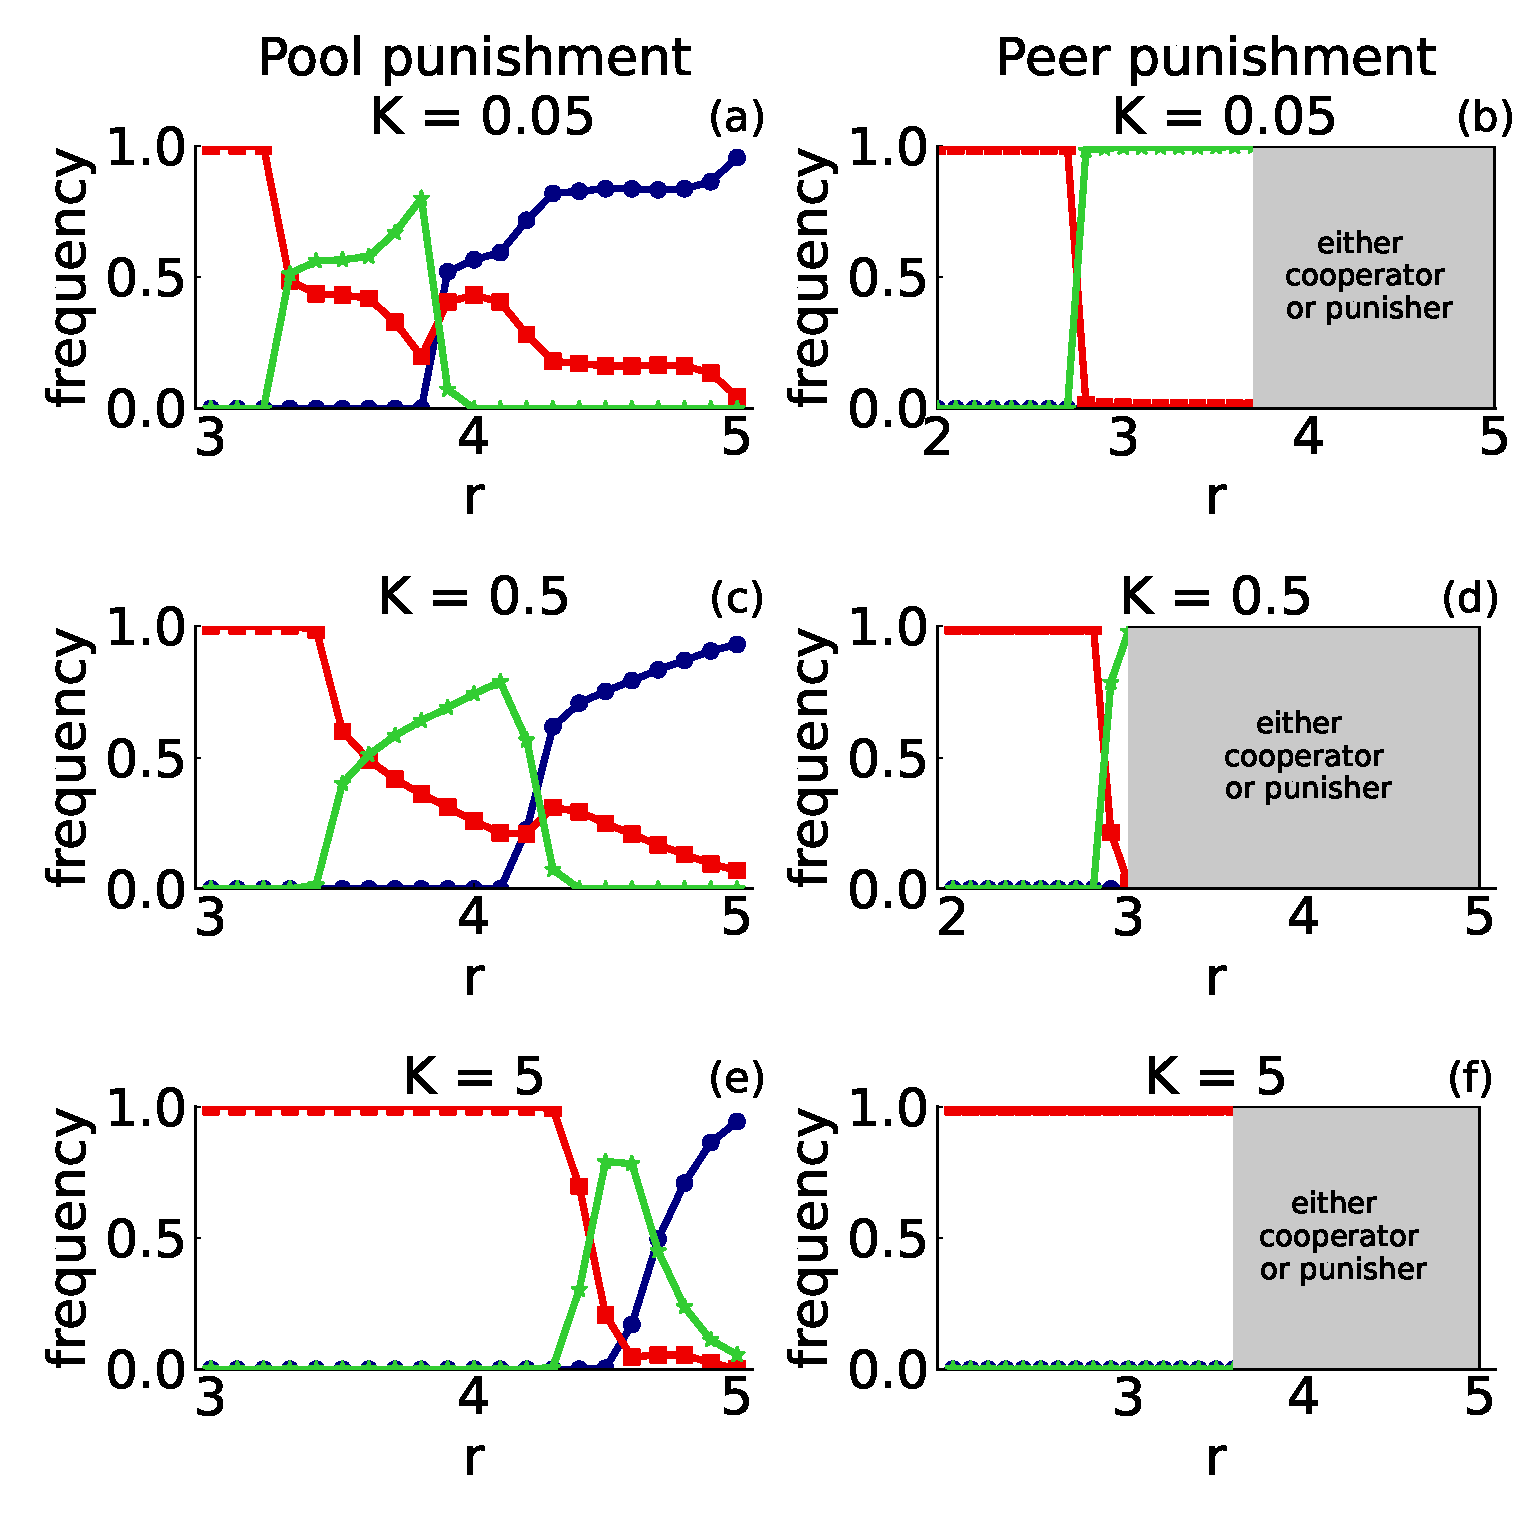
\includegraphics[width=1\linewidth]{Images/P2/densidadVSr_L300t5000variosK.eps}
	\caption{Frequency of each strategy after $5000$ MCS of a PGG simulation as a function of $r$ for different values of the stochastic noise regulator $K$. Cooperators in blue, defectors in red and punishers in green. For greater noise values, cooperation is less profitable. (b) (d) (f) For peer punishment, at some $r$ values defectors become extinct, so  punishers have the same payoff as cooperators. With sufficiently large relaxation times, either punishers or cooperators will go extinct as of neutral drift. (f) For $K=5$ the phase shift between whole domination from defectors and its extinction is very sudden (the step between consecutive $r$ values is $0.1$). The lines are used to guide the eye, and its width is larger than the corresponding error. We have used the following parameter values: $\beta=0.125$, $\gamma=0.0125$.}
	\label{densidad}
\end{figure}




Societies have long used monetary fines to discourage undesirable behavior and promote cooperation. Think of parking tickets, environmental penalties, or business regulations. All these represent ways that communities punish those who do not cooperate with social rules. In our model, we explore two distinct approaches to implementing such punishment: pool punishment and peer punishment. 
In pool punishment, punishers contribute to a common fund. Each time punishers participate in the public goods game, they pay a small amount ($\gamma=0.0125$) into this communal punishment fund. When they encounters a defector, the defector must leave a fine ($\beta=0.125$). Importantly, this fine is applied only once per defector, regardless of how many punishers are in the group.

Peer punishment works differently. Instead of contributing to a central fund, punishers directly confront defectors. Each punisher pays a personal cost (${\gamma=0.0125}$) to punish each defector they encounter, and each defector receives a separate fine ($\beta=0.125$) from each punisher. This can result in more severe punishment when multiple punishers are present.

Both approaches reflects different real-world systems for enforcing cooperation. Pool punishment reflects individuals reporting defectors to a gubernamental enforcement institution, paying taxes to maintaining it. Alternatively in peer punishment, the punishers take a more personal approach conflicting directly with the defectors.


These approaches lead to different mathematical expressions for how individuals fare in the game.

For pool punishment:
\begin{equation}\small
\begin{split}
\text{Cooperators earn: } &\Pi_C^g=\frac{r}{G}(N_C^g+N_P^g)-1 \\
\text{Punishers earn: } &\Pi_P^g=\frac{r}{G}(N_C^g+N_P^g)-1-\gamma \\
\text{Defectors earn: } &\Pi_D^g = \left\{ \begin{array}{ll}
\frac{r}{G}(N_C^g+N_P^g) & \mbox{if $N_P^g=0$} \\
\frac{r}{G}(N_C^g+N_P^g)-\beta & \mbox{if $N_P^g\neq0$}.
\end{array}
\right\}
\end{split}
\end{equation}


For peer punishment, the equations change to reflect the multiple punishments possible:
\begin{equation}
\begin{split}
\text{Cooperators still earn: } &\Pi_C^g=\frac{r}{G}(N_C^g+N_P^g)-1 \\
\text{Punishers now earn: } &\Pi_P^g=\frac{r}{G}(N_C^g+N_P^g)-1-\gamma N_D^g \\
\text{Defectors now earn: } &\Pi_D^g=\frac{r}{G}(N_C^g+N_P^g)-\beta N_P^g.
\end{split}    
\end{equation}



When we simulate these systems over $5000$ generations (Monte Carlo Steps), we observe how different strategies succeed under varying conditions in Fig.~\ref{densidad}. At low enhancement factors $r$, defection dominates because the benefits of cooperation are not high enough to offset its costs. As $r$ increases, punishers begin to thrive because the greater benefits of cooperation make their enforcement role more valuable. At even higher r values, normal cooperators can sometimes outcompete punishers because the high returns make punishment less necessary.

The stochastic noise parameter K influences these patterns significantly. Higher noise levels make cooperation harder to maintain, shifting the transition points toward higher r values. This reflects how uncertainty or imperfect information can make maintaining cooperation more challenging.

Peer punishment shows some particularly interesting dynamics. Under certain conditions, defectors can be completely eliminated. When this happens, punishers and cooperators become equally successful since there's no one left to punish. Then, random chance eventually leads one strategy to dominate through what is called neutral drift. The outcome depends on the relative numbers of punishers and cooperators when defectors disappear, and possibly on their spatial distribution and the system's size.

Comparing the two punishment systems under the same fine $\beta$ and cost $\gamma$ values, peer punishment proves more effective at promoting cooperation. This makes intuitive sense since defectors face multiple fines under peer punishment, making the consequences of non-cooperation more severe.




\section{Varying the enhancement factor as oscillations on time}
\label{3oscillating}


\begin{figure}
	\centering
	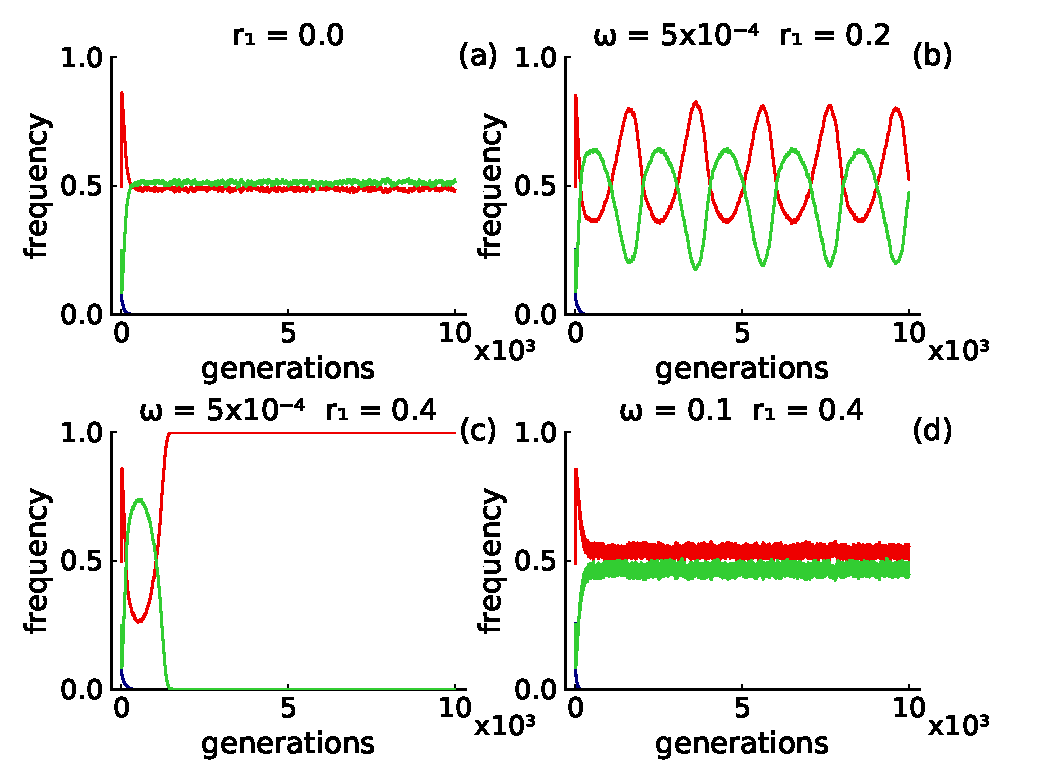
\includegraphics[width=1\linewidth]{Images/P2/freq_tiempo_T0seleccion_Pool.eps}
	\caption{Frequency of each strategy as time passes with an oscillating enhancement factor of the form $r=r_0+r_1\sin(\frac{2\pi \omega}{L^2}t+\delta)$, where  $r_0=3.6$ is the mean value of $r$, $\omega$ is the oscillation frequency in units of MCS$^{-1}$ and $\delta=0$. Results are made in the pool punishment. Cooperators in blue, defectors in red and punishers in green. (a) At the value of $r=3.6$ the punishers and defectors are almost on equal terms rapidly oscillating due to noise. (b) For small oscillation frequencies, the defectors and punishers periodically dominate one another, being the punishers the ones with a greater mean frequency. (c) The amplitude of the oscillation is so big that defectors completely dominate after one cycle. (d) As the oscillation frequency increases, the dynamics is more similar as compared to the case without any $r$ oscillation; while very quick $r$ oscillations, possibly another type of noise, are insignificant to final frequency. We have used the parameter values $\beta=0.125$, $\gamma=0.0125$.}
	\label{oscila}
\end{figure}



\begin{figure}
	\centering
	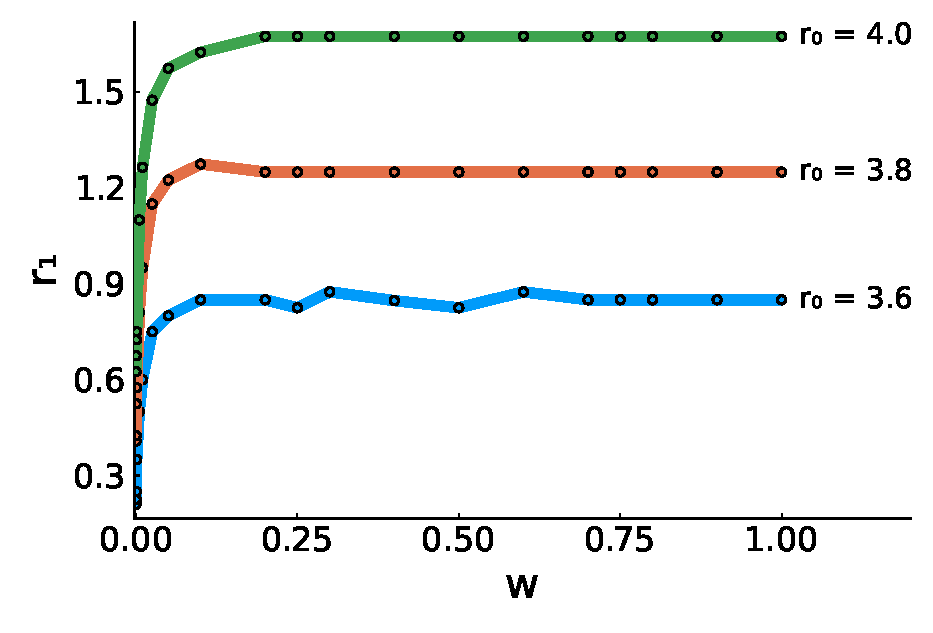
\includegraphics[width=1\linewidth]{Images/P2/grafica_r1_w0_T0_Pool.eps}
	\caption{The figure represents the amplitude $r_1$ of the oscillation $r=r_0+r_1\sin(\frac{2\pi\omega}{L^2}t+\delta)$ for different values of $r_0$, that limits the phase of only defectors (greater amplitudes) and defectors plus punishers (lower amplitudes) in the strict pool punishment regime with a punisher threshold $T=0$. The limiting amplitude $r_1$ grows as $r_0$ raises and, at low oscillation frequencies, when $\omega$ raises. The lines are used to guide the eye, and its width is comparable to the corresponding error. We have used the parameters: $\delta=0$, $\beta=0.125$, $\gamma=0.0125$.}
	\label{r1_w0}
\end{figure}





In real societies, the benefits of cooperation rarely remain constant. Consider investing in a business venture: some days the market soars, other days it plunges. Another example of cooperative activity is farming, which experiences cycles of abundance and scarcity. The public goods game, as typically studied, simplifies this reality by assuming constant returns on cooperation. To better understand how these real-world fluctuations affect cooperation, we need to introduce time-varying returns into our model.

We model these changing investment returns by making the enhancement factor r oscillate over time. While real-world fluctuations can be complex, we start with a simple sinusoidal pattern that captures the essential behavior of periodic changes, a sinusoidal oscillation: $r=r_0+r_1\sin(\frac{2\pi\omega}{L^2}t)$.

The frequency $\omega$, measured in inverse Monte Carlo Steps (MCS$^{-1}$), lets us explore different types of real-world fluctuations. Low frequencies might represent long-term economic cycles, while high frequencies could model rapid fluctuations like daily market volatility or random noise in the system.

When we examine in Fig.~\ref{oscila} how populations evolve under these oscillating conditions, we discover that larger oscillations make it harder for cooperation to survive. When we increase the amplitude $r$, defectors gain an advantage, sometimes even taking over the entire population, as shown in Fig.~\ref{oscila}(c). This suggests that stability, in the sense of predictable returns on cooperation – plays a crucial role in maintaining cooperative behavior.

The frequency of oscillations also matters. When oscillations happen very quickly (Fig.~\ref{oscila}(d)), the population behaves almost as if there were no oscillations at all. This makes intuitive sense: if conditions change faster than people can adapt their strategies, they respond to the average conditions instead.

These findings hold true regardless of whether we use pool or peer punishment, and they persist across different levels of decision-making noise, $K$. The fundamental relationship between instability and reduced cooperation appears to be a robust feature of the system.

To understand exactly when defection becomes dominant, we created Fig.~\ref{r1_w0}. This figure shows the critical amplitude $r_1$ that separates regions where punishers can survive from regions where defectors completely take over, plotted against the oscillation frequency $\omega$ for different values $r_0$. The resulting curve reveals several key insights:

First, the critical amplitude increases with frequency until reaching a plateau. This means that faster oscillations need larger amplitudes to disrupt cooperation completely. At low frequencies, even small oscillations can lead to defector dominance because there are long periods when $r$ dips low enough for defectors to multiply significantly. As frequency increases, the system has less time to respond to each low-$r$ period, requiring larger amplitudes to achieve the same effect.

Second, higher baseline values of $r_0$ push the critical amplitude higher. This makes sense since when cooperation is more profitable on average, it takes larger disruptions to make defection the winning strategy.

We observed these patterns starting from $\omega = 0.00001$, our lowest tested frequency. Interestingly, at even lower frequencies, punishers dominate the system. This occurs because we start our simulations with $\delta = 0$, meaning $r$ initially increases, giving cooperation an early advantage that becomes decisive over very long oscillation periods.

This analysis reveals that cooperation is most vulnerable to slow, large-amplitude changes in the benefits of cooperation. Fast changes, even of large amplitude, have less impact because populations adapt to average conditions. These findings suggest that societies are more resilient to rapid fluctuations in cooperative benefits than to long-term cycles of boom and bust.



\section{Having a delay in punishment}
\label{3delay}



\begin{figure}
	\centering
	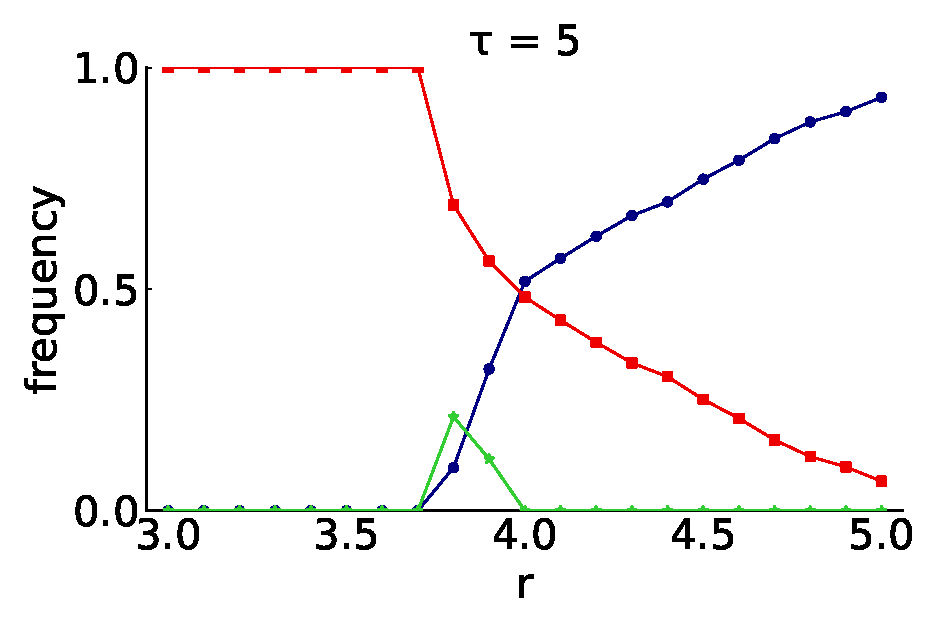
\includegraphics[width=1\linewidth]{Images/P2/densidad_retardo_tau5.0_L100_T0_t5000_Pool.eps}
	
	\caption{
	Frequency of each strategy averaged on the last iterations of a PGG simulation with a delay $\tau=5$ MCS when the defectors are charged with the fine as a function of $r$ in the pool punishment regime. Cooperators in blue, defectors in red and punishers in green. Punishers almost do not appear and defectors are more abundant than on Fig.~\ref{densidad}(c). The lines are used to guide the eye, and its width is larger than the corresponding error. We have used the parameters: $\beta=0.125$, $\gamma=0.0125$, $L=100$. }
	\label{freq_retardo}
\end{figure}

\begin{figure}
	\centering
	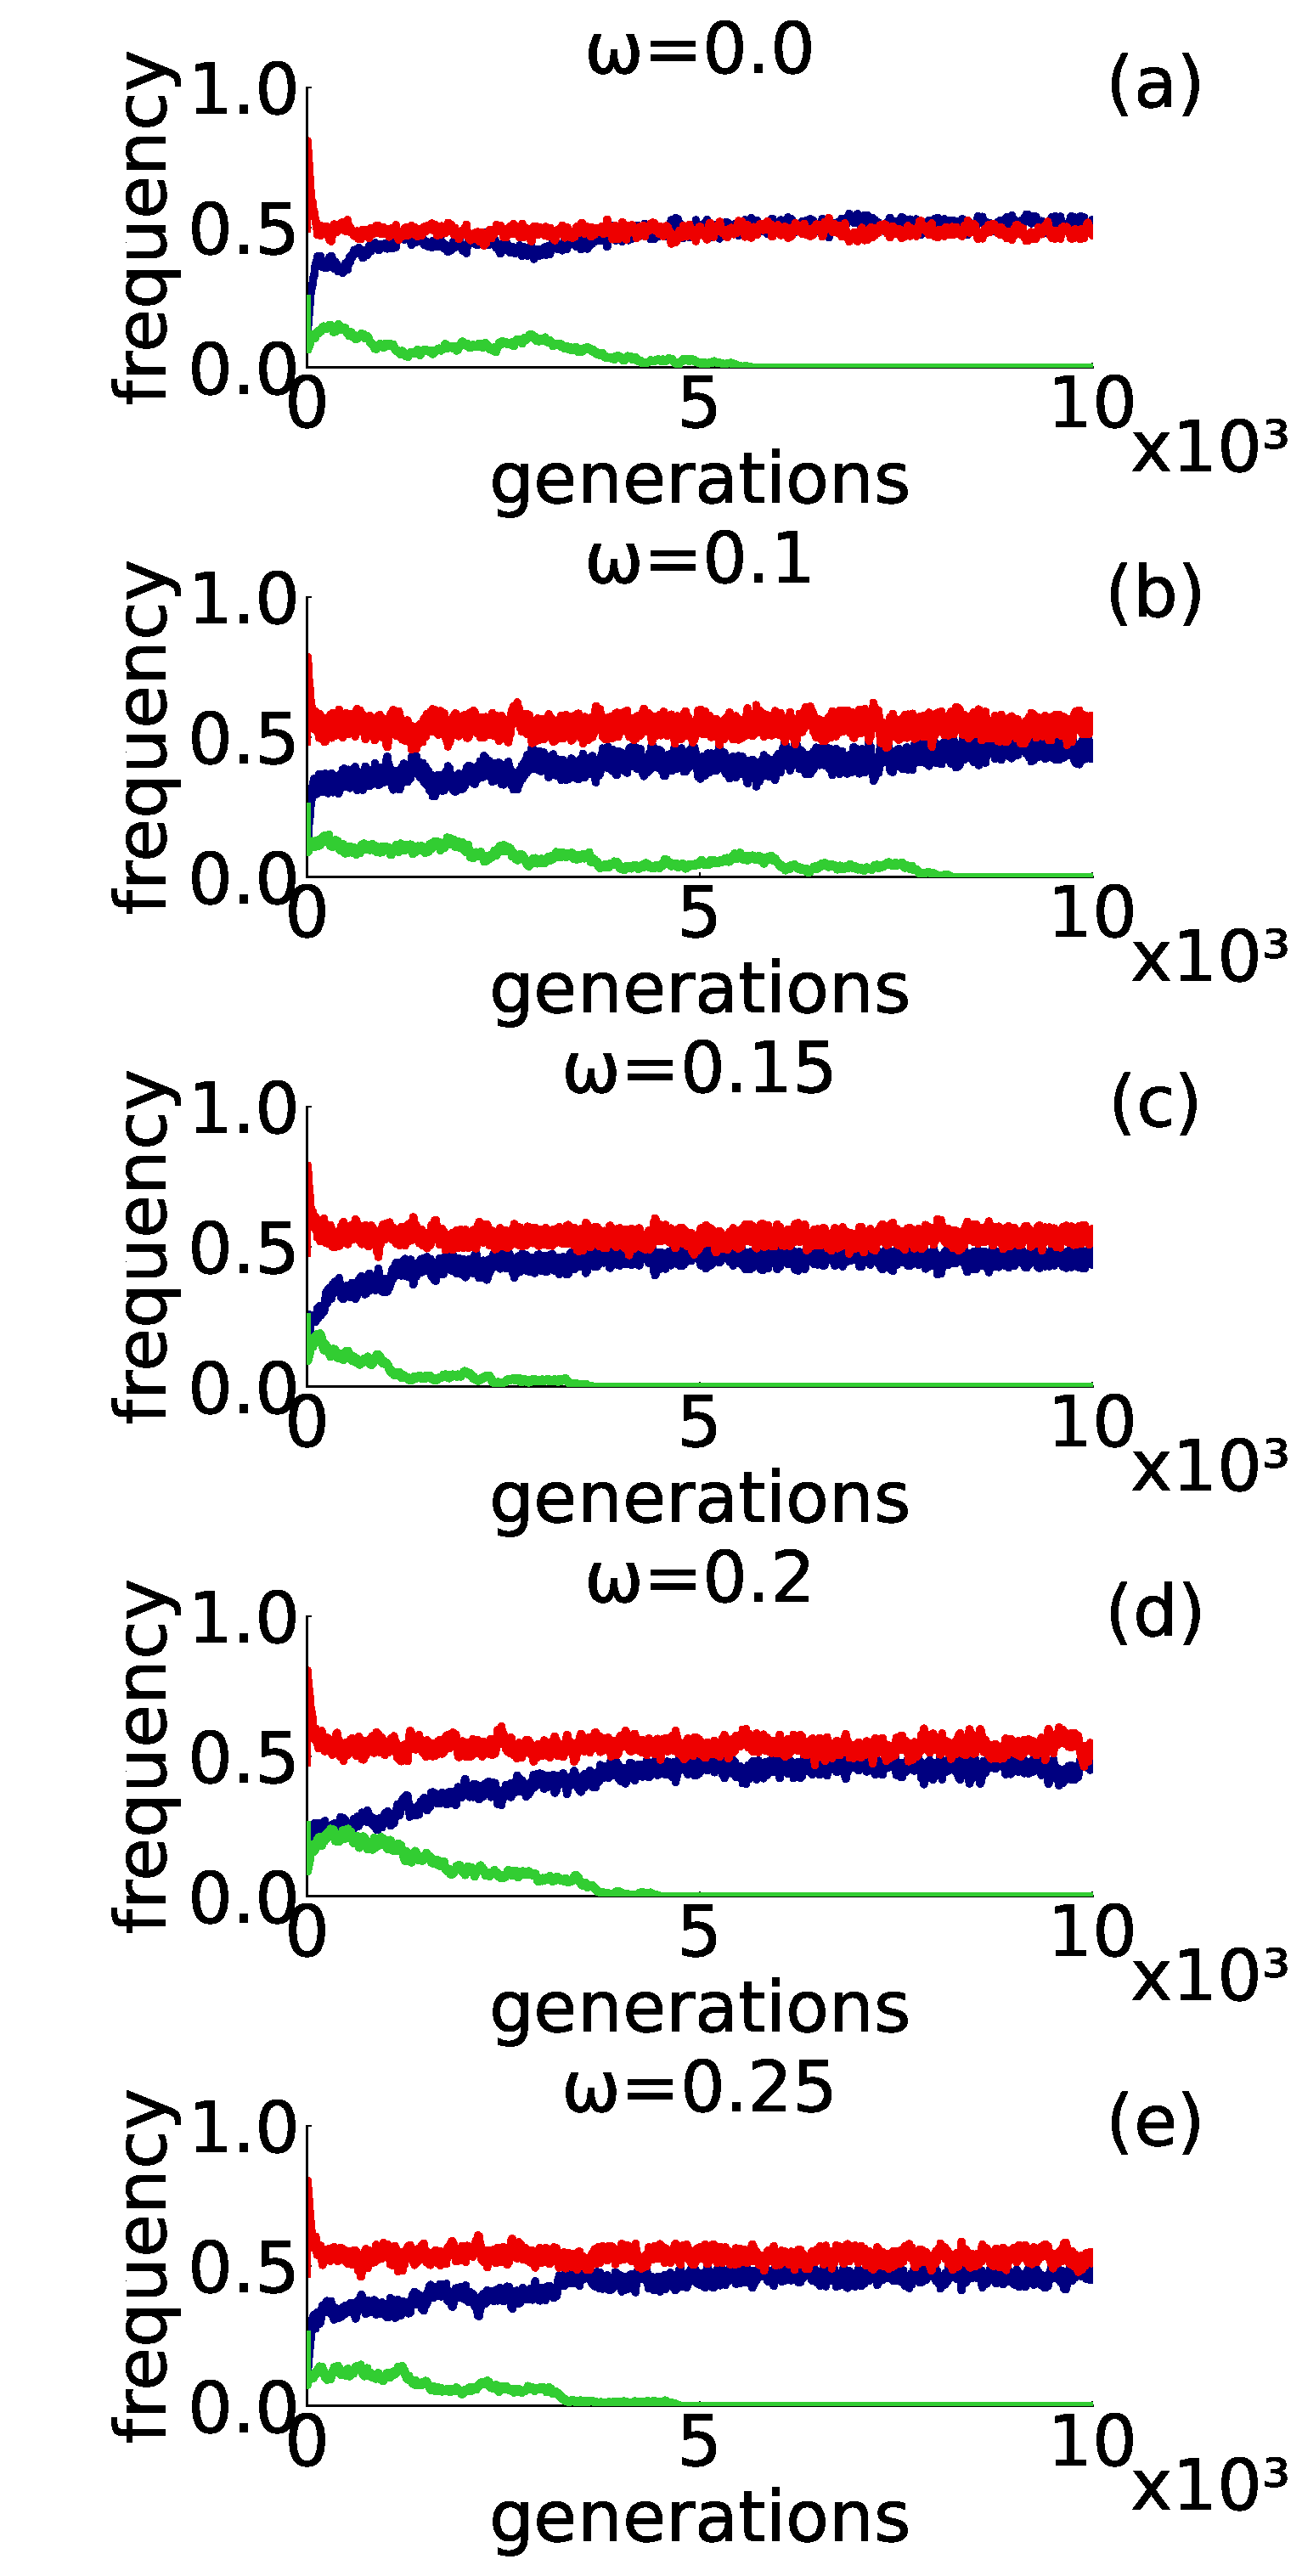
\includegraphics[width=0.6\linewidth]{Images/P2/freq_tiempo_retardoYsin_T0_r04.0_r10.5_tau50000_L100K0.5_t10000.eps}
	\caption{Frequency of each strategy as time passes of a PGG simulation with a delay $\tau=5$ MCS when the defectors are charged with the fine for different oscillation frequencies $\omega$ in the pool punishment regime. (a) No oscillation on the factor $r$. The oscillation of the frequency is due to the delay. With oscillation in the factor $r$, the (b-e) graphics look similar. There is no apparent difference in (d) although $w=0.2=1/\tau$ is the frequency we expected for a resonant behaviour. Cooperators in blue, defectors in red and punishers in green. We have used the parameters: $r_0=4.0$, $r_1=0.5$, $\beta=0.125$, $\gamma=0.0125$.}
	\label{tiempo_retardo_oscilacion}
\end{figure}





In real life, actions and their consequences rarely happen simultaneously. When you speed on the highway, the ticket might arrive weeks later. This delay between action and consequence, or punishment, can significantly affect behavior. Understanding these effects is crucial for designing effective enforcement systems.

To explore how such delays influence cooperation, we modified our model to include a time lag so defectors stay some iterations of the game without receiving the punishment of their infringement.  Punishers detect defection and moments later, defectors actually pay their fines. This delay gives violators a temporary advantage as they can continue benefiting from their behavior before facing consequences.

The added complexity of tracking delayed punishments significantly increased computational demands, so we reduced our population size to L=100 to keep simulation times manageable. Even with this smaller population, the results proved illuminating.

Looking at Fig.~\ref{freq_retardo}, which shows the long-term frequency of each strategy with a delay of $\tau=5$ MCS, we see a dramatic shift from our previous results. Comparing this to Fig.~\ref{densidad}(c) (the no-delay case), we observe two significant changes: (1) Punishers have almost completely disappeared across most values of the enhancement factor $r$. (2) While normal cooperators appear at lower $r$ values than before, defectors maintain a much stronger presence.

This weakening of cooperation makes intuitive sense when we consider how people learn and adapt their behavior. Just as children need to connect punishment directly with their actions to understand consequences, our simulated individuals become less likely to change their behavior when punishment is delayed. The longer the gap between action and consequence, the weaker the learning effect becomes. A principle that holds true whether we use peer punishment or vary the noise in decision-making.

To further understand these delay effects, we investigated whether they might interact with the oscillating returns we studied earlier. Fig.~\ref{tiempo_retardo_oscilacion} shows how populations evolve over time with both delay ($\tau=5$) and oscillating enhancement factors ($r_0=3.8$, $r_1=0.5$) at different frequencies. We were particularly interested in whether we might see resonance, a strengthening of effects, when the oscillation frequency matches the natural frequency created by the delay ($\omega=1/\tau=0.2$).

Nonetheless we found no evidence of such resonance. The population dynamics looked similar across different frequencies, even near the theoretical resonance point as seen in Fig.~\ref{tiempo_retardo_oscilacion}(d). Even more unexpectedly, we didn't observe the periodic oscillations we might have expected given our sinusoidal variation in returns.

What explains this lack of periodicity? Our first thought was that random noise in decision-making might be masking any periodic patterns. However, when we ran simulations in the noiseless regime ($K \to 0$), we still saw no periodic behavior. Then, another account for stocahasticity is the randomness of our Monte Carlo simulation. Specifically, in how we randomly choose which individuals get to update their strategies. This inherent randomness in the update process appears to overwhelm any periodic forcing from our oscillating enhancement factor. Another fact that restrains the observation of oscillation and resonance is the large value of $\omega$, as high-frequency oscillations do not provide with sufficient time for population to adapt. 

This finding highlights an important principle: while both delayed punishment and oscillating returns can independently weaken cooperation, their combined effects do not produce simple, predictable patterns, at least for the parameters studied. A further study with increased range of parameters for larger $\tau$ and smaller $\omega$ values is necessary.




\section{Conclusions }
\label{3Conclusions}


In this chapter, we examined time-dependent effects in the public goods game by adding an additional strategy, the punisher, among cooperators and defectors. Two forms of punishment, peer and pool punishment, were analyzed. While both punishment strategies yielded similar outcomes, peer punishment promoted cooperation more effectively. This greater efficacy comes from the fact that defectors are penalized multiple times for the same infraction, leading to a cumulative punishment effect.

To explore the dynamical nature of the game, we introduced a time-dependent enhancement factor $r$ and a time delay $\tau$ in the application of punishment to defectors. Both mechanisms were found to have a negative effect in cooperation. Large oscillation amplitudes led to an increase in the population of defectors, as oscillations in productivity disrupted the stability of cooperative behavior. For high oscillation frequencies, the system's behavior resembled that of a non-oscillatory scenario, suggesting that rapid oscillations, similar to noise, have minimal impact.

When a time delay in punishment was introduced, the effectiveness of punishment diminished, resulting in higher levels of defection. Thus, delayed punishment also impairs cooperation. 





\begin{thebibliography}{04}

\bibitem{CoopBio}
L. A. Dugatkin,
Cooperation in animals: An evolutionary overview
Biol. and Philos. \textbf{17}, 459–476, (2002).
\url{https://doi.org/10.1023/A:1020573415343}

\bibitem{CoopSocial}
P. Kollock, Social dilemmas: the anatomy of cooperation,
Annu. Rev. Sociol. \textbf{24}, 183-214 (1998).
\url{https://doi.org/10.1146/annurev.soc.24.1.183}

\bibitem{CoopEconomy}
R. Schaap and Andries Richter,
Overcapitalization and social norms of cooperation in a small-scale fishery,
Ecol. Econ. \textbf{166}, 10643 (2019).
\url{https://doi.org/10.1016/j.ecolecon.2019.106438}

\bibitem{SocialPhy}
\raggedright
M. Jusup, P. Holme, K. Kanazawa,  M. Takayasu, B. Podobnik, L. Wang,  W. Luo, T. Klanjšček, J. Fan,  S. Boccaletti, and M. Perc,
Social physics.
Phys. Rep. \textbf{948}, 1--148 (2022). 
\url{https://doi.org/10.1016/j.physrep.2021.10.005}

\bibitem{RPSCooperation} 
Z. Bi and H. Zhou, Optimal Cooperation-Trap Strategies for the Iterated Rock-Paper-Scissors Game, PLoS One \textbf{9}, e111278 (2014). \url{https://doi.org/10.1371/journal.pone.0111278}

\bibitem{Prisionero} 
G. Szabó and C. Töke, Evolutionary Prisoner’s Dilemma Game on a Square Lattice, Phys. Rev. E \textbf{58}, 69 (1998). \url{https://doi.org/10.1103/PhysRevE.58.69}

\bibitem{PublicGoods} 
M. Archetti and I. Scheuring, Game Theory of Public Goods in One-Shot Social Dilemmas Without Assortment, J. Theor. Biol. \textbf{299}, 9 (2012). \url{https://doi.org/10.1016/j.jtbi.2011.06.018}

\bibitem{r/G} 
T. Wu, F. Fu, and L. Wang, Partner Selections in Public Goods Games with Constant Group Size, Phys. Rev. E \textbf{80}, 026121 (2009). \url{https://doi.org/10.1103/PhysRevE.80.026121}

\bibitem{EdgeRule} 
X. Sun, Y. Li, H. Kang, Y. Shen, J. Peng, H. Wang, and Q. Chen, Co-Evolution of Complex Network Public Goods Game under the Edges Rules, MDPI Entropy \textbf{22}, 199 (2020). \url{https://doi.org/10.3390/e22020199}






\bibitem{Migration} 
D. Helbing and W. Yu, The Outbreak of Cooperation among Success-Driven Individuals under Noisy Conditions, Proc. Natl. Acad. Sci. U.S.A. \textbf{106}, 3680 (2009). \url{https://doi.org/10.1073/pnas.0811503106}

\bibitem{Reputation} 
Z. Wang, L. Wang, Z. Yin, and C. Xia, Inferring Reputation Promotes the Evolution of Cooperation in Spatial Social Dilemma Games, PLoS One \textbf{7}, e40218 (2012). \url{https://doi.org/10.1371/journal.pone.0040218}

\bibitem{Reward} 
Y. Li, S. Chen, and B. Niu, Reward Depending on Public Funds Stimulates Cooperation in Spatial Prisoner’s Dilemma Games, Chaos Solitons Fractals \textbf{114}, 38 (2018). \url{https://doi.org/10.1016/j.chaos.2018.07.002}

\bibitem{SocialExclusion} 
T. Sasaki and S. Uchida, The Evolution of Cooperation by Social Exclusion, Proc. R. Soc. B \textbf{280}, 20122498 (2013). \url{https://doi.org/10.1098/rspb.2012.2498}

\bibitem{Punish2} 
A. Szolnoki, G. Szabó, and M. Perc, Phase Diagrams for the Spatial Public Goods Game with Pool Punishment, Phys. Rev. E \textbf{83}, 036101 (2011). \url{https://doi.org/10.1103/PhysRevE.83.036101}

\bibitem{Late} 
I. Waichman and L. Stenzel, When Punishment Strikes Late: The Effect of a Delay in Punishment and Punishment Feedback on Cooperation and Efficiency, J. Neurosci. Psychol. Econ. \textbf{12}, 1 (2019). \url{https://doi.org/10.1037/npe0000099}

\bibitem{ValorK} 
A. Szolnoki, M. Perc, and G. Szabó, Topology-Independent Impact of Noise on Cooperation in Spatial Public Goods Games, Phys. Rev. E \textbf{80}, 056109 (2009). \url{https://doi.org/10.1103/PhysRevE.80.056109}




\end{thebibliography}







\clearemptydoublepage



%\chapter{Measuring complexity in evolutionary games with the Hamming distance}
\label{chap:HammingGames}




\begin{quotation}

	\vspace{-3cm}
    \begin{flushright}
    \begin{minipage}[t][5cm][b]{0.5\textwidth}
    {\letquote ``We should not judge people by their peak of excellence; but by the distance they have traveled from the point where they started."}
    
    \bigskip
    
    -{\small  Henry Ward Beecher}
    \end{minipage}
    \end{flushright}
    
    \vspace{0.5cm}
\end{quotation}

%TODO sequencia



Physicist have studied evolutionary game dynamics for their complex dynamics. From simple rules, complex behavior can be observed emerging from population size. Here we are interested in the complex pattern formation first discovered by May and Nowak in 1992 \cite{SpatialChaos}. They studied the prisoner's dilemma where players were organized in a square grid and each round played games with their immediate neighbors. Each player was set to be either a cooperator or a defector, which determined the payoff they got each game. Then the payoff was summed through every game they played that round. After each round, the players adapted the strategy of the individual with better payoff. For a parameter region they observed complex patterns when plotting in different colors cooperators and defectors.

One can easily see the difference between two configurations of cooperators and defectors by measuring the Hamming Distance. This measures the number of different elements between two groups of elements of same size. It was introduced
by Richard Hamming in 1950 in \cite{HammingOrigins}. Since then it has been very helpful for computer science and cryptography, but its uses are broader. In the context of social games the Hamming distance has also been used, \cite{HammingSocial1, HammingSocial2}.

Moreover in \cite{HammingChaos1,HammingChaos2}, the Hamming distance is used to asses complexity on social games. The authors measure the difference between two close configurations of rock-paper-scissors models that describe stochastic network simulations of the May and Leonard type. The Hamming distance converged to a certain value. But the distance oscillated increasing amplitude towards zero or the population size when shifting a parameter that represents the mobility beyond a critical point. For these parameter regime one strategy will end up being the only one present, and by varying just one individual's strategy at the beginning, the outcome can change completely, changing which strategy ends up winning.  This shows that the susceptibility to  initial perturbations of the system. 

In this chapter we summarize the results of a study \cite{Alfaro2024} where we measured the complexity of the patterns observed by May and Nowak in \cite{SpatialChaos} through this same method, by analyzing the Hamming distance between two initially close configurations of players. We found that for the parameter region where May and Nowak found the complex patterns, the Hamming distance grew in time as a sigmoid until it reached a convergence value; and for the rest of values, the distance quickly decreased to zero. This shows that the divergence of the Hamming distance could be an indicator of complex behavior. 

We also studied the divergence of the Hamming distance in a different game, the public goods game. This time there was a certain degree of stochasticity in the game, which led to the growth of the Hamming distance for all cases. This means that our algorithm does not distinguish random processes from chaotic ones. However the growth was more rapid for some values which may indicate a higher complexity for those cases.


\section{Prisoner's Dilemma}

We developed a tool to asses the complexity of dynamic social games. The first thing to do is to check its validity with a game we know, presents complex behavior. This is the case for the game studied by May and Nowak in \cite{SpatialChaos}, the prisoner's dilemma, PD. 

\subsection{Model}

The first game studied was the prisoner's dilemma. This is a game between two players that can be reproduced with the payoff matrix of Table~\ref{tab:PayoffMatrix} under $T>R>P>S$.



\begin{table}[H]
\centering
\label{tab:PayoffMatrix}
    \begin{tabular}{c|c c}
        ~& ~C~ & ~D~  \\
        \hline
        ~C~ & R & S  \\
        ~D~ & T & P
    \end{tabular}
\caption{Payoff matrix for pairwise social games. $C$ and $D$ stands for the options of the players, either cooperate or defect. Players gain the reward payoff $R$ if both cooperate, the punish reward $P$ if both defect, and the temptation $T$ or the sucker $S$ payoff if one defects while the other defects.}
\end{table}



 We have set $R = 1$, the payoff if both players cooperate; $P = 0$, the payoff if both defect; $T > 1$,  the payoff for a defector playing against a cooperator, which gains $S = 0$. Because the risk-averting dilemma strength results in $D_r= P - S = 0$ this setup is a boundary game, not fully representing the PD. We have chosen this setup to reproduce the exact conditions observed by May and Nowak in \cite{SpatialChaos}.


\begin{figure}
    \centering
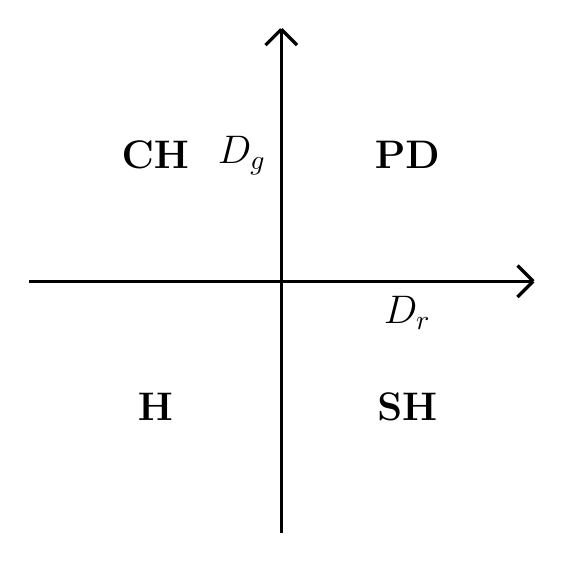
\begin{tikzpicture}

%axis
\draw[very thick] (-3.2,0) -- (3.2,0);
\draw[very thick] (0,-3.2) -- (0,3.2); 

%quiver heads
\draw[very thick] (-0.2,3) -- (0,3.2);
\draw[very thick] (0.2,3) -- (0,3.2);

\draw[very thick] (3,-0.2) -- (3.2,0);
\draw[very thick] (3,0.2) -- (3.2,0);

\draw (-0.5,1.6) node {\Large{$D_g$}};
\draw (1.6,-0.4) node {\Large{$D_r$}};

\draw (-1.6,1.6) node {\Large{\textbf{CH}}};
\draw (1.6,1.6) node {\Large{\textbf{PD}}};
\draw (1.6,-1.6) node {\Large{\textbf{SH}}};
\draw (-1.6,-1.6) node {\Large{\textbf{H}}};

\end{tikzpicture}
    \caption{Diagram representing the four types of pairwise social games according to dilemma strength. CH stands for the Chicken game, PD for the Prisoner's Dilemma, SH stands for the Stag-hunt game and H stands for Harmony game. }
    \label{fig:SocialGames}
\end{figure}


The risk-adverting dilemma strength, together with the gamble-intending dilemma strength $D_g = T - R$ composes the map of types of games pairwise social games represented in Fig.~\ref{fig:SocialGames}. These games are the harmony game, where $D_r,D_g < 0$, no dilemma is found and the logic option is to cooperate; the stag hunt game with, $D_r > 0, D_g < 0$ where the logic option is to do the same as your opponent; the chicken game with $D_r < 0, D_g > 0$, where the logic option is to do the opposite than your opponent; and finally the prisoner's dilemma with $D_r,D_g > 0$ where the logic option is to defect. However if both cooperated they would have better than both defecting but the temptation $T$ is higher than the reward $R$, thus promoting the tragedy of the commons and receiving their punishment $P$ \cite{TragedyCommons}.

Each player is put in a square grid with periodic boundaries, and plays eight games with their Moore neighbors, Fig.\ref{fig:Moore2Neigh}. Then they sum the payoff gained in all those games and compare the result with their neighbors and copy the strategy of the one with greater total payoff in that round. This is done for all players simultaneously and repeated through time. 


\begin{figure}
\centering
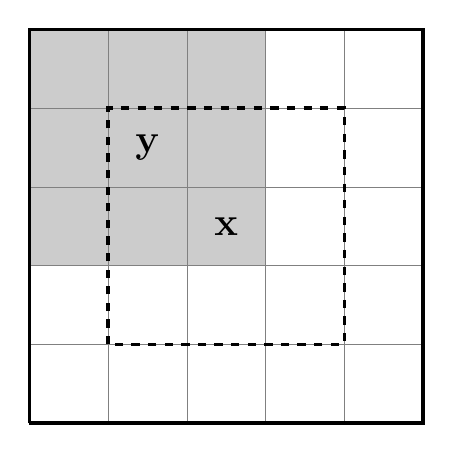
\begin{tikzpicture}


\fill[gray!40!white] (0,2) rectangle (3,5);


\draw[step=1cm,gray,very thin] (0,0) grid (5,5);

\draw[very thick] (0,0) -- (0,5) -- (5,5) -- (5,0) -- (0,0);
\draw[dashed, very thick] (1,1) -- (1,4) -- (4,4) -- (4,1) -- (1,1);

\draw (2.5,2.5) node {\Large{\textbf{x}}};
\draw (1.5,3.5) node {\Large{\textbf{y}}};


\end{tikzpicture}
\caption{Agent $x$'s strategy is affected by the payoff of all agents in his Moore neighborhood (inside the dashed line); for example agent $y$, whose payoff depends of his own Moore neighborhood (shaded region). Therefore, the strategy of the agent $x$ depends on all $25$ agents in his second Moore neighborhood (inside the bold line).}
\label{fig:Moore2Neigh}
\end{figure}





We plot cooperators in blue and defectors in red in Fig.\ref{fig:PD_Sequencia}. These plots show spatio-temporal chaotic patterns that evolve quickly. In \cite{SpatialChaos} the authors claimed them to be fractal-like structures. However, as we can see on Fig.\ref{fig:GranPlot}, when we augment the population size $N$, the patterns do not scale, and instead the clusters all size similarly.




\begin{figure}
    \centering
    \includegraphics[width=0.8\linewidth]{Images/P3/PD_Secuencia.png}
    \caption{Snapshots of the public goods game at $4$ different times of cooperators in blue, defectors in red, and agents that have changed from the previous configuration in yellow. The snapshots are taken at instants $t1 = 1000$, $t2 = 1002$, t3 = $1004$ and $t4 = 1006$ after one defector is introduced at the center in a sea of cooperators in a grid of $101\times101$ agents with periodic boundaries.}
    \label{fig:PD_Sequencia}
\end{figure}


\begin{figure}
    \centering
    
\includegraphics[width=1\linewidth]{Images/P3/PD_GranPlot.eps}
    \caption{Cooperators and defectors in blue and red, respectively.}
    \label{fig:GranPlot}
\end{figure}















The authors of \cite{SpatialChaos} made an observation that the patterns seemed chaotic for these values of the temptation reward, $1.8 < T < 2$. We want a tool that quantifies the complexity of the pattern evolution that presents spatio-temporal chaos. We think that the algorithm we have developed, described in the following subsection, serves as an indicator for complex behavior and provides a value that quantifies how quickly the patterns evolve, which may be related to the Lyapunov time.



\subsection{Hamming distance measure}


The Hamming distance measures the difference between two objects as the number of different elements they contain. Think of two matrices or vectors of the same size, the Hamming distance between is the number of elements that differ from each position. Now we can represent the configuration of cooperators and defectors at each time as a matrix of $0$'s and $1$'s. Then we can calculate the Hamming Distance of two configurations by subtracting them and taking absolute values since they are binary matrices.

When we do so we observe that the distance quickly goes to zero for simulations in all parameter regimes except for values of the temptation reward in $1.8 < T < 2$, where it growths until it saturates at a given value that augments with population size as we can see in Fig.~\ref{fig:HammingTimePopulation_PD}. We can analytically calculate this value, since it is the statistical Hamming distance, that two random configurations of $0$'s and $1$'s with certain probabilities would have. This value is proportional to the population size, and is calculated as:
\begin{equation}
H_{stat}(t)=N_C(t)p_D(t)+N_D(t)p_C(t),
\end{equation} 
where $N_C$ and $N_D$ indicate the number of cooperators and defectors; and $p_C$ and $p_D$, the proportion of them. Since the proportion of cooperators and defectors is the number of them divided by the total population, we find that the 
proportionality constant for the saturation values of the Hamming distance is
\begin{equation}
h_{stat}(t)=p_C(t)p_D(t)+p_D(t)p_C(t),
\end{equation} 
which, in the case of binary strategies, it can be simplified as:
\begin{equation}
h_{stat}(t)=2p_C(t)(1-p_C(t)).
\end{equation} 

This value could be time dependent, but since the system is stable, the proportions of cooperators and defectors follow the Nash equilibrium and depend only on the values of $T$.



\begin{figure}
	\centering
	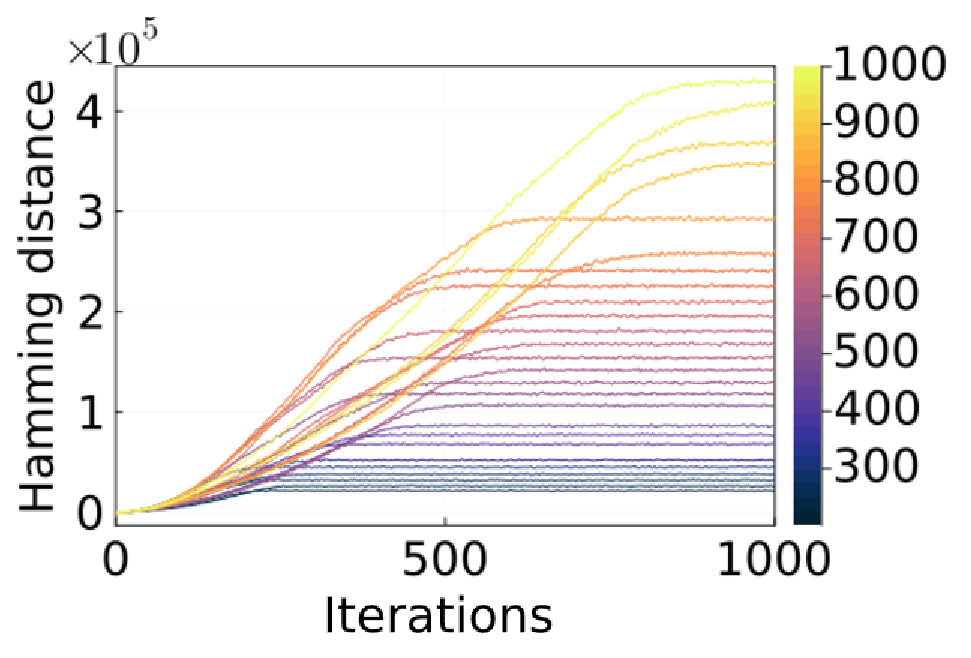
\includegraphics[width=0.8\linewidth]{Images/P3/HammingTimePopulation_PD.eps}
	\caption{Hamming distance of the the two solutions of the prisoner's dilemma versus time. Different colors represent different values of the grid size $L$. The larger the grid size, the longer it takes for the Hamming distance to reach the saturation value $H_{stat}$.}
	\label{fig:HammingTimePopulation_PD}
\end{figure}






Then, if we normalize the Hamming distance from Fig.~\ref{fig:HammingTimePopulation_PD}, dividing it by $H_{stat} = h_{stat}*N$, we get the normalized Hamming distance in Fig.~\ref{fig:NormalHammingTimePopulation_PD}. This figure shows sigmoids with different growth rate. Larger population sizes take longer to reach the saturation value.



\begin{figure}
	\centering
	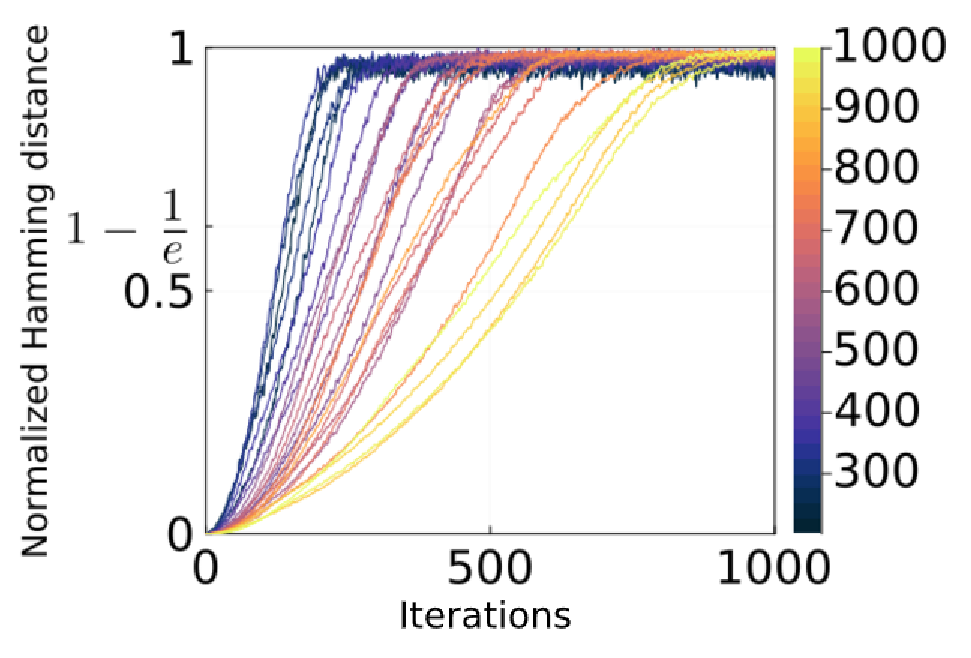
\includegraphics[width=0.8\linewidth]{Images/P3/NormalHammingTimePopulation_PD.eps}
	\caption{ Normalized Hamming distance of the two solutions of the prisoner's dilemma versus time. Multiple curves are shown with different colors, representing the different grid size $L$ values. The curves grow in a sigmoid-like curve towards one. They are normalized to the statistical Hamming distance which depends on L. The larger $L$ is, the longer it takes for the normalized Hamming distance to reach $1$.}
	\label{fig:NormalHammingTimePopulation_PD}
\end{figure}


\begin{figure}
	\centering
	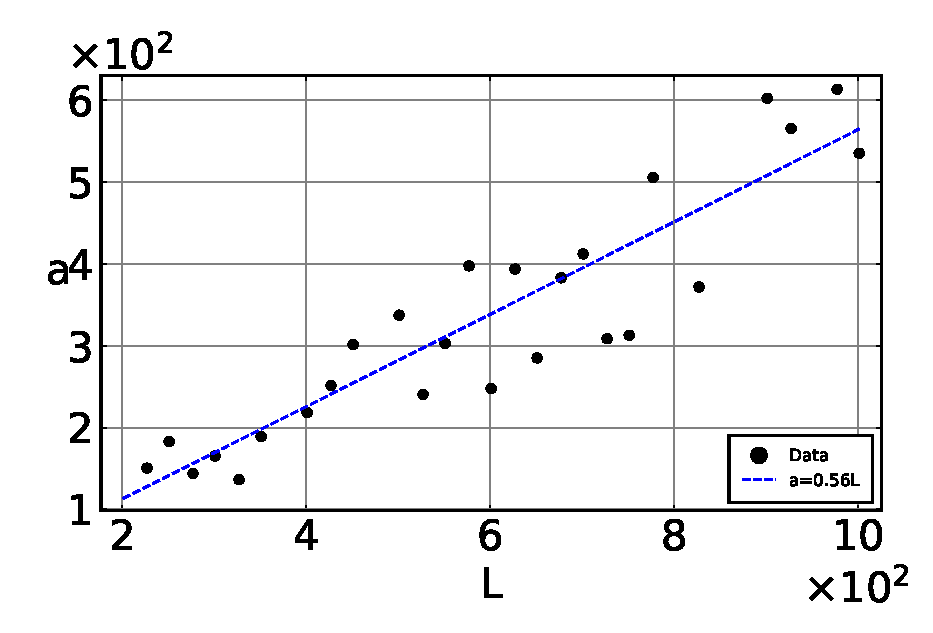
\includegraphics[width=0.8\linewidth]{Images/P3/aVSL_PD.eps}
	\caption{Parameter $a$ from the Weibull ``stretched exponential" function $F(t;k,a)=1-e^{-(t/a)^k}$ fitted to the normalized Hamming distance of the solutions for the prisoner's dilemma versus grid size $L$. It shows a linear regression (dashed blue line) where $a$ grows proportionally to $L$.}
	\label{fig:aVSL_PD}
\end{figure}





We have fitted this curves to the Weibull "stretched exponential" function \cite{Weibull}
\begin{equation}
    F(t;k,a)=1-e^{-(t/a)^k},
    \label{WeibullDistr}
\end{equation}
where $a$ is the timescale of growth and $k$ tells how abrupt the growth is. We chose this function because it is the most simple sigmoid function that values zero at the origin and converge to one, having only two relevant parameters.

The value of $a$ can be seen as something similar to the Lyapunov time, and as seen on Fig.~\ref{fig:aVSL_PD}, it is proportional to the grid size $L$, with a slope of $0.56 \pm 0.05$ and a neglible intercept. Note that the population size is $N = L^2$. The maximum slope is $0.5$, since at maximum velocity any change in the agent's strategy propagates to two agents away as seen on Fig.\ref{fig:Moore2Neigh}. The measured value of the slope is near the maximum which indicates a great propagation of the mismatches, and that may be related to complex behavior. As for the values of $k$, every curve is around $k = 2.5\pm0.4$.




\begin{figure}
\centering
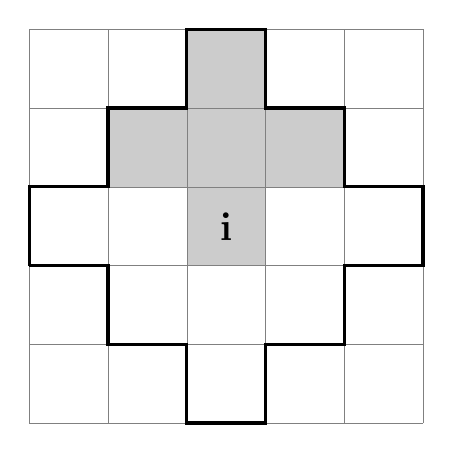
\begin{tikzpicture}

\fill[gray!40!white] (2,2) rectangle (3,5);
\fill[gray!40!white] (1,3) rectangle (4,4);

\draw[step=1cm,gray,very thin] (0,0) grid (5,5);

\draw[very thick] (0,2) -- (0,3) -- (1,3) -- (1,4) -- (2,4) -- (2,5) -- (3,5) -- (3,4) -- (4,4) -- (4,3) -- (5,3) -- (5,2) -- (4,2) -- (4,1) -- (3,1) -- (3,0) -- (2,0) -- (2,1) -- (1,1) -- (1,2) -- (0,2);

\draw (2.5,2.5) node {\Large{\textbf{i}}};


\end{tikzpicture}
\caption{Von Neumann neighborhood at a distance $2$ of agent $i$. The individual $i$ plays $5$ games with agents in cross-like patterns like the one shaded.}
\label{fig:VonNeumman2Neigh}
\end{figure}



\section{Public Goods Game}

Now that we have checked that our algorithm can asses the complexity in the PD, we want to measure weather the game we studied in the previous chapter was chaotic. The public goods game, PGG. 

\subsection{Model}

This time, to make the model simpler we only allow the cooperate and defect strategy, and leave out the punish strategy. The rest of the model we leave the same. That is, agents play $5$ games along $4$ other agents among their second Von Neumann neighbors,Fig.~\ref{fig:VonNeumman2Neigh} and their payoff depends whether they are cooperators, $\Pi_C$, or defectors, $\Pi_D$ and the number of cooperators $N_C^g$ that there are in their group.

\begin{equation}
    \begin{split}
    	&\Pi_C^g=\frac{r}{G}\cdot N_C^g-1 \\
    	&\Pi_D^g=\frac{r}{G}\cdot N_C^g
    \end{split}    
\end{equation}

Here $r$ is a parameter that rewards cooperation and $G = 5$ is the size of the group.

Then, the accumulated payoff $\Pi=\sum_g^G \Pi^g$ determines the fitness of each agent in an evolutionary model where a random agent chooses whether to adopt or not the strategy of a random neighbor. This time we wanted to reduce the stochasticity. Therefore, this time, if the accumulated payoff of the agent's neighbor is greater, it adopts its strategy. Whereas if it is lesser, it does nothing. Nonetheless we still maintained the random election of the agent that will change its strategy to maintain the same game as previous chapter, where the parameter of noise $K$ is in the limit of $K \to 0$.


\begin{figure}
	\centering
	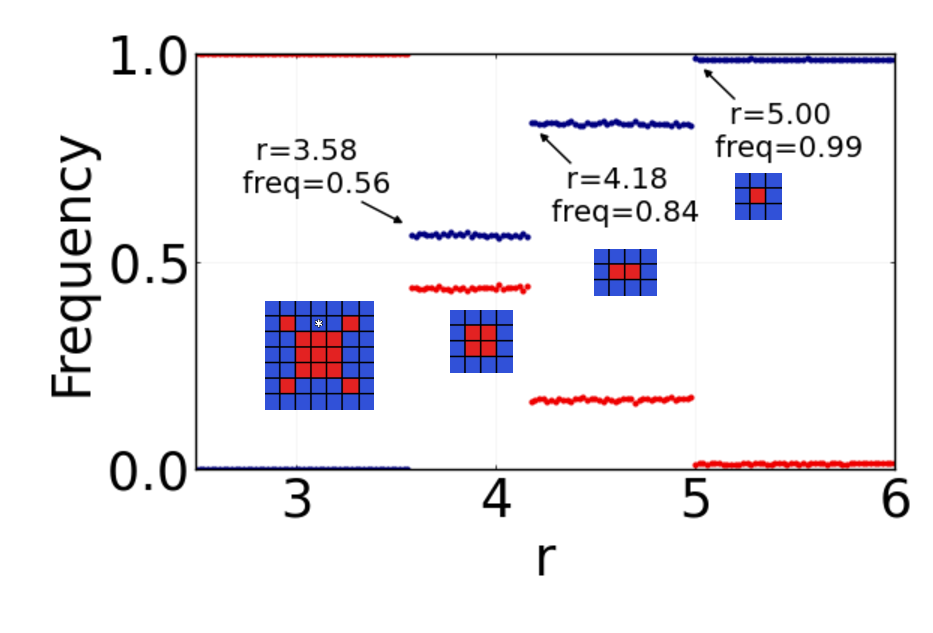
\includegraphics[width=1\linewidth]{Images/P3/PGG_Proportion.eps}
	\caption{Proportion of cooperators (in blue) and defectors (in red) after running a simulation of the public goods game starting with a random strategy in each of the $N=90000$ agents with a relaxation time of $2000$ generations. We can see that the proportion changes only at some values of $r$. This values have been calculated analytically. Each shifts corresponds to a change on whether the surrounding cooperators have greater or lesser payoff than the surrounded defectors in the configurations we show. For the first configuration this holds strictly for the white-marked cooperator and the defector below it at the first shift at $r=25/7\approx3.57$.}
	\label{fig:PGG_Proportion}
\end{figure}


Under these rules, we observe that after a transitory period, the average population stabilizes with  cooperator and defector proportions given by Fig.~\ref{fig:PGG_Proportion}. It shows that the proportion only changes at some values of $r$ and then stays constant. We are able to predict the values of $r$ where these shifts appear analytically. We just have to compare the payoff of the defectors and the cooperators that surround them in configurations that are clusters of defectors of different sizes that are shown in the figure.

As an example here we have the payoff of the white marked cooperator in the first configuration and the defector below it.

\begin{equation}
    \begin{split}
    	&\Pi_C=\frac{1}{5}(5r+4r+2\times3r+r)-5=\frac{16}{5}r-5 \\
    	&\Pi_D=\frac{1}{5}(4r+2\times2r+r+0)=\frac{9}{5}r
    \end{split}
\end{equation}

When we equal these two payoffs we get that the value of $r$ where we expect a shift is $r=25/7\approx3.57$, which is indeed where we find the shift. The next shifts can be calculated similarly with the rest of the configurations and give values of $25/6=4.1\hat6$, $25/5=5$ and $25/3=8.\hat3$.


In the PGG cooperation is a Nash equilibrium for $r\geq5$. At the Nash equilibrium  the payoff cannot be increased when changing strategy given that the rest of agents don't change theirs. But we observe that for $5<r<8.\hat3$ cooperation is not the only strategy present. This is because the payoff of each agent is affected by the strategies of its neighbors. Therefore, a defector surrounded by cooperators has greater payoff than them, even though it would have greater payoff if it were a cooperator. This means that being at a Nash equilibrium does not eliminate all defectors. We observe a last shift at $r=8.\hat3$, beyond this last shift defection is not viable.  We don't show this shift in Fig.\ref{fig:PGG_Proportion} because it can hardly be appreciated at the current scale (from a cooperator proportion of $0.99$ to $1$). What's more, since the election of the agent that changes its strategy is at random, the computational times for all defectors to adopt the cooperation strategy are large.





\subsection{Hamming distance measure}


To asses the complexity of our PGG we measured the Hamming distance of two initially close configurations differing of only one agent. Because the election of the agent that adopt a new strategy in the evolutionary model is chosen at random, we have to make sure every random interaction is chosen the same through both simulations.


We can see how mismatches propagate in Fig.~\ref{fig:SequenciaHamming}. For each snapshot both configuration, the original and the copy with a different agent at the center, are plotted on the same space in two layers with one layer being slightly transparent. The defectors in one configuration are ploted red and in the other, green. This allows us to watch how the mismatches propagate. They do so radially and at constant velocity on average, but following the branches of defectors when watched closely.


\begin{figure}
    \centering
    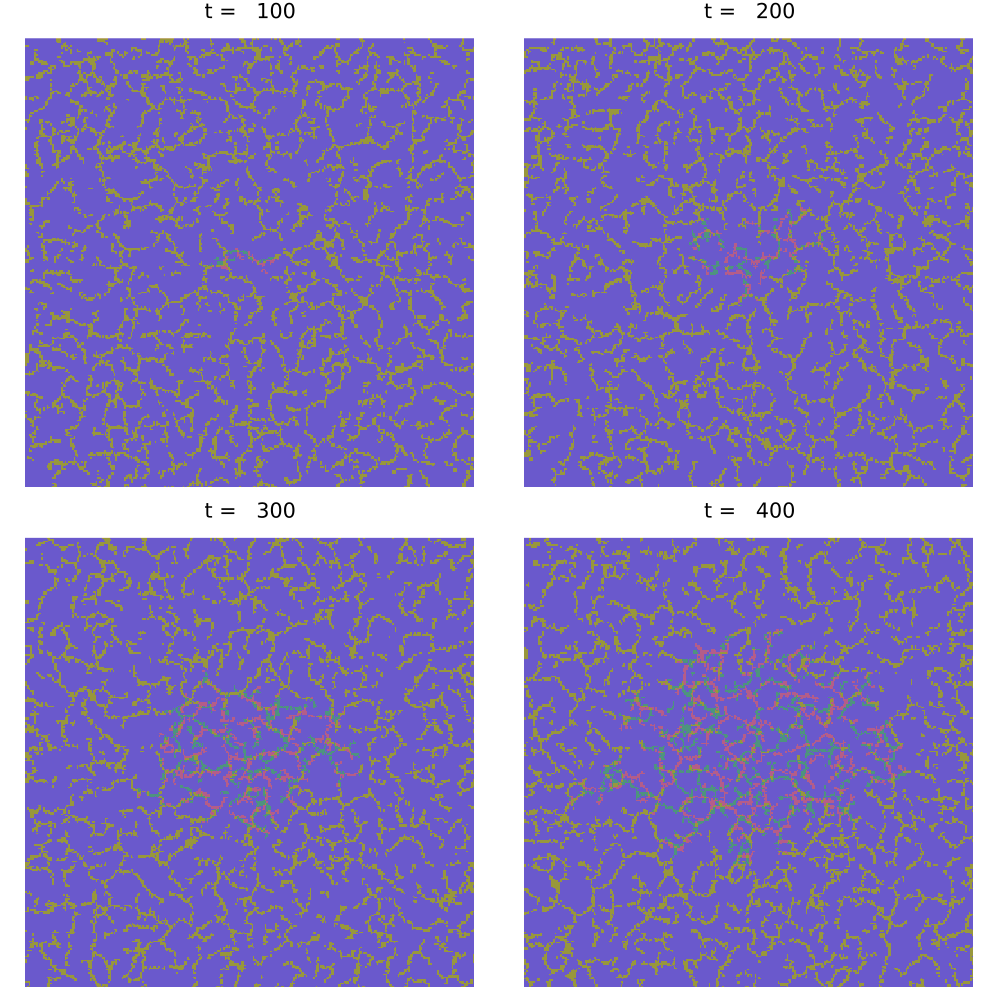
\includegraphics[width=0.8\linewidth]{Images/P3/PGG_SecuenciaHamming.png}
    \caption{Snapshots at $4$ different times of both configurations (original, and copy with altered agent at $t = 0$ at the center) of the public goods game. Cooperators are plotted in blue, defectors in red for one configuration and in green for the other. Both configurations are plotted one on top of the other with a transparent effect. Thanks to this we can see that the mismatches propagate at average constant velocity and expand radially.}
    \label{fig:PGG_SequenciaHamming}
\end{figure}





\begin{figure}
	\centering
	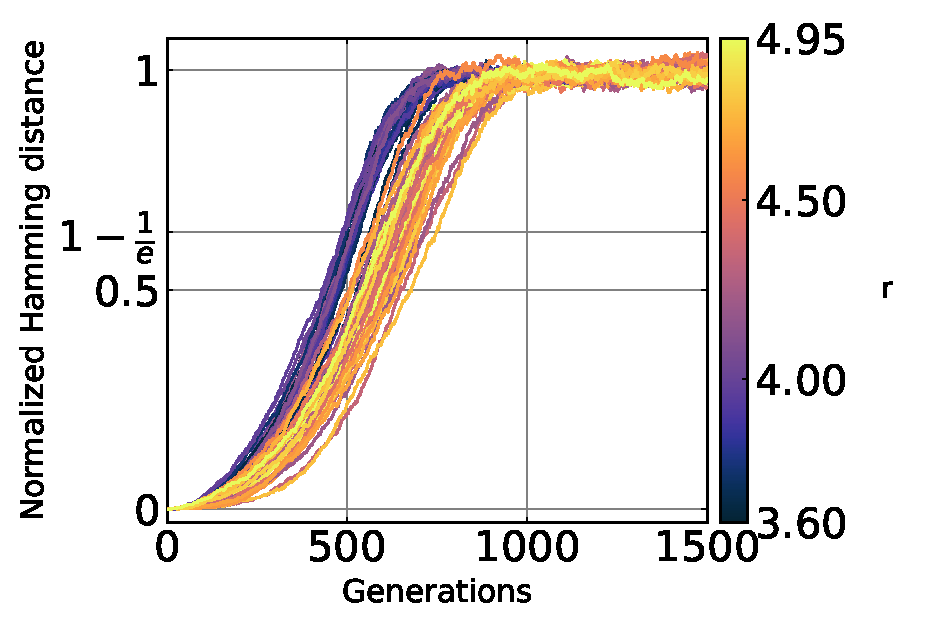
\includegraphics[width=1\linewidth]{Images/P3/NormalHammingTimePopulation_r.eps}
	\caption{Normalized Hamming distance between the solutions for the public goods game versus time. Multiple curves are shown with different colors, representing the different $r$ values. The curves grow in a sigmoid-like curve towards one. They are normalized to the statistical Hamming distance, which depends on $r$, so curves ranging from  $25/7\leq r<25/6$ are normalized to a different value than those at $25/6\leq r<5$. There is a distinction between the two regimes, the curves of the first one (blue ones) reach its midpoint earlier than the ones in the second regime (orange ones).}
	\label{fig:NormalHammingTimePopulation_r}
\end{figure}



\begin{figure}
	\centering
	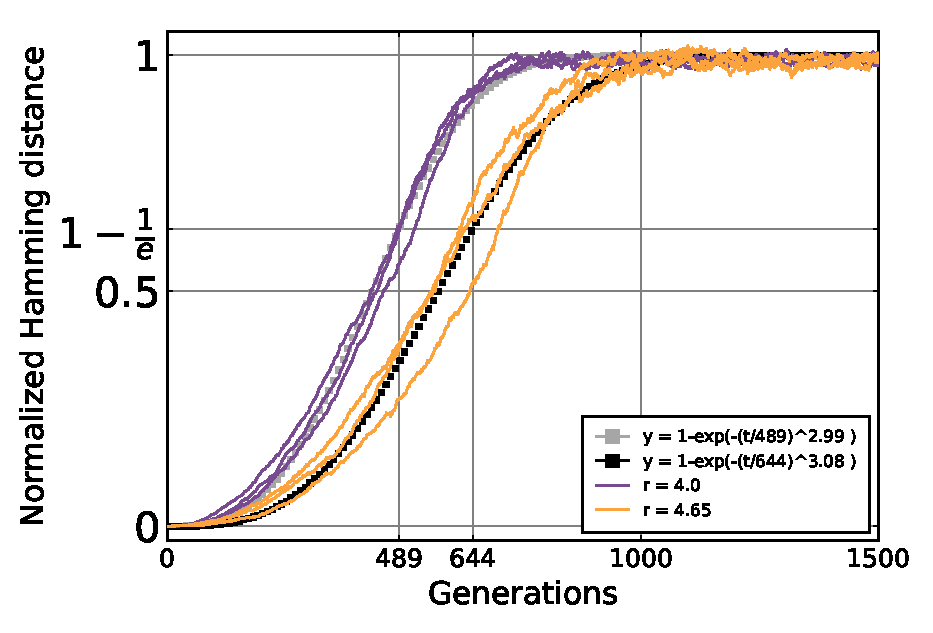
\includegraphics[width=1\linewidth]{Images/P3/NormalHammingTimePopulation_2r.eps}
	\caption{Normalized Hamming distance between the solutions for the public goods game versus time. Different colors represent two different $r$ values. They are normalized to the statistical Hamming distance, which depends on $r$, so the two curves are normalized to a different value. The Weibull ``stretched exponential" function $F(t;k,a)=1-e^{-(t/a)^k}$ is fitted to the curves and we observe different values of $a$, which can be seen as similar to the Lyapùnov time. The $r=4$ curves (blue and left ones), representing the regime $25/7\leq r<25/6$ has a lower value of $a$ than the curves with $r=4.65$ (orange and right ones). This indicates that, for $25/7\leq r<25/6$, the system is more sensitive to initial conditions.}
	\label{fig:NormalHammingTimePopulation_r}
\end{figure}


The result was, as seen in Fig.\ref{fig:NormalHammingTimePopulation_r} that the Normalized Hamming distance grew as a sigmoid like in the previous section for values of the parameter $r$ between $25/7\approx3.57$ and $8.\hat3$. These are all the values where there are present cooperators and defectors . We cannot say that this is an indicator of chaos this time, because probably, what the algorithm is assessing is the randomness in the election of agent to change its strategy. Nonetheless, when we fit the curves to the Weibull ``stretched exponential" function in Fig.\ref{fig:NormalHammingTimePopulation_2r}, we get lower values of $a$ for curves in the first regime, $25/7\leq r<25/6$. This means that the system is more susceptible to changes in the initial conditions. For values of $5>r>8.\hat3.$ we get a very large value of $a = 3685$.


\section{Conclusions}

We have developed an algorithm to measure the divergence of two binary configurations of cooperators and defectors in the prisoner's dilemma and the public goods game using the Hamming distance. We observed that if the game has no random elements, the divergence can be linked to complex behavior.
The Hamming distance grew as a sigmoid function in time for a system that was clear, had a complex behavior and was zero when not.
 
We also calculated a measure that could correlate to a Lyapunov time. The measure, which indicated approximately the midpoint of the sigmoids, was proportional to the grid size and the constant of proportionality was near its maximum for the prisoner's dilemma with no random elements.

For the public goods game with some random elements, all games studied presented a divergence of the Hamming distance. Nonetheless, the divergence was slower, it took longer to reach the midpoint, for some games, which had a sparse population of defectors and a great number of cooperators.

Even though our studied was focused on two particular cases, we are sure the algorithm is adequate to measure divergence and stability in many systems and geometries due to the simplicity of its implementation. In fact, in the next chapter we explain how we used the same tool to make a classification of elementary cellular automata based on complexity.

 




\begin{thebibliography}{04}

\bibitem{Alfaro2024}
G. Alfaro and M. A. F. Sanjuán,
Hamming distance as a measure of spatial chaos in evolutionary games,
Phys. Rev. E \textbf{109}, 014203 (2024)
\url{10.1103/PhysRevE.109.014203}


\bibitem{SpatialChaos}
M. A. Nowak and R. M. May,
Evolutionary games and spatial chaos. 
Nature \textbf{359}, 826--829 (1992).
\url{https://doi.org/10.1038/359826a0}

\bibitem{HammingOrigins}
\raggedright
R.Hamming,
Error detecting and error correcting codes.
Bell Syst. Tech. J. \textbf{29}, 147--160 
(1950)
\url{https://doi.org/10.1002/j.1538-7305.1950.tb00463.x}


\bibitem{HammingSocial1}
\raggedright
R. D'hulst and G. J. Rodgers,
The hamming distance in the minority game.
Physica A \textbf{270}, 514--525 (1999) 
\url{https://doi.org/10.1016/S0378-4371(99)00211-3}

\bibitem{HammingSocial2}
\raggedright
J.-W. Kim,
A tag-based evolutionary prisoner's dilemma game on networks with different topologies.
JASSS, \textbf{13}, 2 (2010)
\url{https://doi.org/10.18564/jasss.1584}

\bibitem{HammingChaos1}
\raggedright
D. Bazeia, M. B. P. N. Pereira, A. V. Brito, B. F. Oliveira, and J. G. G. S. Ramos,
A novel procedure for the identification of chaos in complex biological systems.
Sci. Rep. \textbf{7}, 44900 (2017)
\url{https://doi.org/10.1038/srep44900}

\bibitem{HammingChaos2}
\raggedright
D. Bazeia, J. Menezes, B. F. De Oliveira, and J. G. G. S. Ramos,
Hamming distance and mobility behavior in generalized rock-paper-scissors models.
EPL \textbf{119}, 58003 (2017)
\url{https://doi.org/10.1209/0295-5075/119/58003}

\bibitem{TragedyCommons}
\raggedright
G. Hardin,
The tragedy of the commons: the population problem has no technical solution; it requires a fundamental extension in morality.
Science \textbf{162}, 1243--1248 (1968)
\url{https://doi.org/10.1126/science.162.3859.1243}


\bibitem{Weibull}
\raggedright
W. Weibull, A statistical distribution function of wide applicability.
J. Appl. Mech. \textbf{18}, 293--297 (1951).
\url{https://hal.science/hal-03112318v1}

\end{thebibliography}

\clearemptydoublepage


\chapter{Elementary cellular automata and Hamming distance}
\label{chap:HammingECA}

\renewcommand\labelenumi{(\roman{enumi})}
\renewcommand\theenumi\labelenumi


\begin{quotation}
	\vspace{-3cm}
    \begin{flushright}
    \begin{minipage}[t][5cm][b]{0.5\textwidth}
    {\letquote ``Automation is good, so long as you know exactly where to put the machine."}
    
    \bigskip
    
    -{\small  Eliyahu Goldratt}
    \end{minipage}
    \end{flushright}
    
    \vspace{0.5cm}
\end{quotation}

\vspace{0.5cm}

%\bibitem{Alfaro2024}
G. Alfaro and M. A. F. Sanjuán,
Classification of cellular automata based on the Hamming
distance,
Chaos \textbf{34}, 083129 (2024)
\url{https://doi.org/10.1063/5.0227349}

\vspace{1cm}


In the previous chapter we reviewed evolutionary social games and configured them for agents to play in a square lattice with their neighbors. We calculated the payoff of each individual according to some rules and then they adopted the strategy of one of its neighbors depending on the payoff. Since the payoff of the agents depends only on the state of their neighbors, if we do not allow error of decision (i.e. with the decision-making Rule-$K \to 0$), then each combination of neighboring agents will produce unambiguously the updated state of the central agent at the next iteration. Therefore, if we have the prisoner's dilemma with Moore neighborhood as in last chapter, the state of an agent depends only on the state of all its $24$ neighbors and its own. 

One could obtain all of the possible results of the game with the different combinations of these $25$ agents. Given that each agent can only be either a cooperator or a defector, we get $2^{25}$ different situations that completely define the system. If now we would get the state of the current cell at the next iteration for each of these situations, then we would have formalized the game as a cellular automaton. The rules of this automaton would be each of the combinations of the neighborhood cells states. That would be $2^{25}$ rules to follow, which would make a very complicated cellular automaton, although one could get the same behavior with a lower number of rules by intelligently making more complicated rules. 

For this study we use the algorithm developed in the investigation of the previous chapter, but this time with implement it on elementary cellular automata, the most simple cellular automata.

But, what exactly is a cellular automaton?

\section{Cellular Automata}


A cellular automaton, or CA, is a collection of rules that determine the dependence of cells' states to the state of neighboring cells.
Usually, CA do not have a rule for every combination of states of cells, but have a few rules that univocally tells each cell how to update. Take for example Conway's Game of Life. With only four rules that check weather a certain number of neighboring cells are alive or dead, (1 or 0), the state of each cell is determined. With only these four rules the system presents a broad complexity, with complex patterns arising from simple initial configurations. 


There are different methods to increase the complexity of cellular automata. One could let the cells have more than two states, like the first ever studied cellular automata, which was developed in the late 1950s by John von Neumann~\cite{VonNeummanCA} and had 29 states per cell. It was developed as a model for discrete liquid motion, but he was also interested in the idea of self-replication and how machines could replicate themselves. With this automata he made a universal constructor. Additionally increasing the spatial dimensions of the system would complicate the dynamics. One could also let the automata have memory by allowing the rules to depend on the state of cells at previous iterations.

This complexity arising from simple rules has given rise to the thorough research of CA in many ambits of science. For example, in physics they have been used to model the circulation of vehicles,~\cite{PhysicsCA1}, and pedestrians~\cite{PhysicsCA2}. In~\cite{PhysicsCA3} a model for discrete lattice gases are cellular automata. The authors of~\cite{PhysicsCA4} use a set of cellular automata to simulate avalanches in sand piles. Cellular automata has also been used in quantum mechanics,~\cite{PhysicsCA5}. They have also been studied in engineering to implement logical devices as in~\cite{EngineeringCA1}. In cryptography they are widely used as in~\cite{CryptographyCA1, CryptographyCA2Lya}. Multiple applications have also been found in biology,~\cite{BiologyCA1, BiologyCA2, BiologyCA3}


To measure this complexity we will use, again, the Hamming distance, but in order of understanding better the limitations of this distance for measuring complexity, here we study the simpler case of CA, the Elementary Cellular Automata, or ECA. 







\begin{table}
\centering
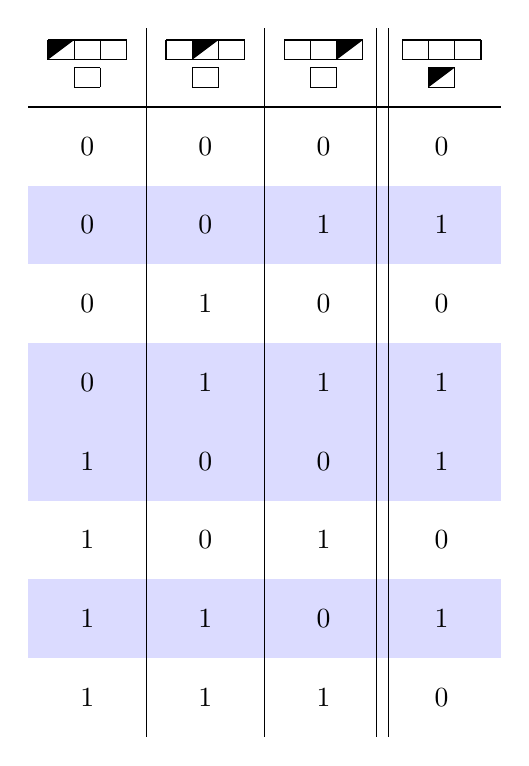
\begin{tikzpicture}

%color

\fill[blue!14!white] (-0.5*1.5,-0.5) rectangle (3.5*1.5,-1.5);
\fill[blue!14!white] (-0.5*1.5,-2.5) rectangle (3.5*1.5,-4.5);
\fill[blue!14!white] (-0.5*1.5,-5.5) rectangle (3.5*1.5,-6.5);

% values of cells

\draw (0*1.5,0) node {0};
\draw (1*1.5,0) node {0};
\draw (2*1.5,0) node {0};
\draw (3*1.5,0) node {0};

\draw (0*1.5,-1) node {0};
\draw (1*1.5,-1) node {0};
\draw (2*1.5,-1) node {1};
\draw (3*1.5,-1) node {1};

\draw (0*1.5,-2) node {0};
\draw (1*1.5,-2) node {1};
\draw (2*1.5,-2) node {0};
\draw (3*1.5,-2) node {0};

\draw (0*1.5,-3) node {0};
\draw (1*1.5,-3) node {1};
\draw (2*1.5,-3) node {1};
\draw (3*1.5,-3) node {1};

\draw (0*1.5,-4) node {1};
\draw (1*1.5,-4) node {0};
\draw (2*1.5,-4) node {0};
\draw (3*1.5,-4) node {1};

\draw (0*1.5,-5) node {1};
\draw (1*1.5,-5) node {0};
\draw (2*1.5,-5) node {1};
\draw (3*1.5,-5) node {0};

\draw (0*1.5,-6) node {1};
\draw (1*1.5,-6) node {1};
\draw (2*1.5,-6) node {0};
\draw (3*1.5,-6) node {1};

\draw (0*1.5,-7) node {1};
\draw (1*1.5,-7) node {1};
\draw (2*1.5,-7) node {1};
\draw (3*1.5,-7) node {0};

% esquemas
    % 1
        % horizontal
\draw (-0.5,1.35) -- (0.5,1.35);
\draw (-0.5,1.1) -- (0.5,1.1);

\draw (-0.5+1/3,1) -- (-0.5+2/3,1);
\draw (-0.5+1/3,0.75) -- (-0.5+2/3,0.75);

        % vertical
\draw (-0.5,1.35) -- (-0.5,1.1);
\draw (-0.5+1/3,1.35) -- (-0.5+1/3,1.1);
\draw (-0.5+2/3,1.35) -- (-0.5+2/3,1.1);
\draw (-0.5+1,1.35) -- (-0.5+1,1.1);

\draw (-0.5+1/3,1) -- (-0.5+1/3,0.75);
\draw (-0.5+2/3,1) -- (-0.5+2/3,0.75);

        %triangle
 \node (A) at (-0.5,1.35) {};
 \node (B) at (-0.5,1.1) {};
 \node (C) at (-0.5+1/3,1.35) {};

\fill[fill=black] (A.center)--(B.center)--(C.center);

    % 2
        % horizontal
\draw (-0.5+1.5,1.35) -- (0.5+1.5,1.35);
\draw (-0.5+1.5,1.1) -- (0.5+1.5,1.1);

\draw (-0.5+1/3+1.5,1) -- (-0.5+2/3+1.5,1);
\draw (-0.5+1/3+1.5,0.75) -- (-0.5+2/3+1.5,0.75);

        % vertical
\draw (-0.5+1.5,1.35) -- (-0.5+1.5,1.1);
\draw (-0.5+1.5+1/3,1.35) -- (-0.5+1/3+1.5,1.1);
\draw (-0.5+1.5+2/3,1.35) -- (-0.5+2/3+1.5,1.1);
\draw (-0.5+1.5+1,1.35) -- (-0.5+1+1.5,1.1);

\draw (-0.5+1/3+1.5,1) -- (-0.5+1/3+1.5,0.75);
\draw (-0.5+2/3+1.5,1) -- (-0.5+2/3+1.5,0.75);

        %triangle
 \node (A) at (-0.5+1.5+1/3,1.35) {};
 \node (B) at (-0.5+1.5+1/3,1.1) {};
 \node (C) at (-0.5+1.5+2/3,1.35) {};

\fill[fill=black] (A.center)--(B.center)--(C.center);


    % 3
        % horizontal
\draw (-0.5+3,1.35) -- (0.5+3,1.35);
\draw (-0.5+3,1.1) -- (0.5+3,1.1);

\draw (-0.5+1/3+3,1) -- (-0.5+2/3+3,1);
\draw (-0.5+1/3+3,0.75) -- (-0.5+2/3+3,0.75);

        % vertical
\draw (-0.5+3,1.35) -- (-0.5+3,1.1);
\draw (-0.5+3+1/3,1.35) -- (-0.5+1/3+3,1.1);
\draw (-0.5+3+2/3,1.35) -- (-0.5+2/3+3,1.1);
\draw (-0.5+3+1,1.35) -- (-0.5+1+3,1.1);

\draw (-0.5+1/3+3,1) -- (-0.5+1/3+3,0.75);
\draw (-0.5+2/3+3,1) -- (-0.5+2/3+3,0.75);

        %triangle
 \node (A) at (-0.5+3+2/3,1.35) {};
 \node (B) at (-0.5+3+2/3,1.1) {};
 \node (C) at (-0.5+3+1,1.35) {};

\fill[fill=black] (A.center)--(B.center)--(C.center);


    % 4
        % horizontal
\draw (-0.5+4.5,1.35) -- (0.5+4.5,1.35);
\draw (-0.5+4.5,1.1) -- (0.5+4.5,1.1);

\draw (-0.5+1/3+4.5,1) -- (-0.5+2/3+4.5,1);
\draw (-0.5+1/3+4.5,0.75) -- (-0.5+2/3+4.5,0.75);

        % vertical
\draw (-0.5+4.5,1.35) -- (-0.5+4.5,1.1);
\draw (-0.5+4.5+1/3,1.35) -- (-0.5+1/3+4.5,1.1);
\draw (-0.5+4.5+2/3,1.35) -- (-0.5+2/3+4.5,1.1);
\draw (-0.5+4.5+1,1.35) -- (-0.5+1+4.5,1.1);

\draw (-0.5+1/3+4.5,1) -- (-0.5+1/3+4.5,0.75);
\draw (-0.5+2/3+4.5,1) -- (-0.5+2/3+4.5,0.75);

        %triangle
 \node (A) at (-0.5+4.5+1/3,1) {};
 \node (B) at (-0.5+4.5+1/3,0.75) {};
 \node (C) at (-0.5+4.5+2/3,1) {};

\fill[fill=black] (A.center)--(B.center)--(C.center);


%lines

\draw (-0.5*1.5,0.5) -- (3.5*1.5,0.5);

\draw (0.5*1.5,1.5) -- (0.5*1.5,-7.5);
\draw (1.5*1.5,1.5) -- (1.5*1.5,-7.5);

\draw (2.45*1.5,1.5) -- (2.45*1.5,-7.5);
\draw (2.55*1.5,1.5) -- (2.55*1.5,-7.5);
\end{tikzpicture}
\caption{Truth table of ECA Rule-$90$. At the right, the state of the central cell at the next iteration for each of the configurations gives the name to the rule. From top to bottom: $0\times1 + 1\times2 + 0\times4 + 1\times8 + 1\times16 + 0\times32 + 1\times64 + 0\times128 = 90$  }
\label{tab:Rule90}

\end{table}









\subsection{Elementary Cellular Automata}

ECA are one-dimensional, binary CA that depend only on the first neighbors. Therefore all the different results of all the combinations of three cells which can have only two states are $2^{2^3} = 256$ which is the number of different ECA rules. Due to symmetry reasons, of all of these rules only $88$ are inequivalent. The rest produce either the same result or the complementary than one of those $88$ rules. 




ECA rules are recognized by a number from $0$ to $255$. The rules are named as follows. Take each combination of 0s and 1s of the three cells. Order them ascendingly, by the value of the binary number if the leftmost cell represents the value of $2^2$ the central cell the value of $2^1$ and the rightmost, $2^0$. Now, the state of the cell for the next iteration of the eight combinations given each rule forms a binary number. This number, translated to decimal, names the rule. This is exemplified in Table~\ref{tab:Rule90}.


From the mid 1980s Stephen Wolfram classified all CA in four classes~\cite{WolframCA_ClassOrigen}. This phenomenological classification studied the behaviour of all the rules of Elementary Cellular Automata with various initial conditions. Ordered by increasing complexity, the classes are:





\begin{enumerate}
    \item Class-$1$: The automata in this class quickly evolve to a homogeneous and stable state.
    \item Class-$2$: In this class the automata quickly evolve to a periodic state.
    \item Class-$3$: The patterns that form in the evolution of the automata in this class are pseudo-random or chaotic and never repeat, except for Poincaré recurring times. That is, for automata with finite population size $L$ there is only $2^L$ possible states.
    \item Class-$4$: The automata in this class are complex in the sense that there are regions where the evolution is periodic that mix with regions that behave like those at Class-$3$. Since this regions are in contact they affect each other in a very long complex evolution that may end after a long time into a periodic state like automata at Class-$2$. 
\end{enumerate}




We can observe this graphically in Fig.~\ref{fig:4classes}.

Different initial conditions may evolve to different behaviour, and be classified as a different class, so a sufficient number of initial conditions should be necessary for a cellular automaton to be classified at each class.

Class 4 is the most interesting ones, with examples like ECA Rule-$110$ and Conway's Game of Life, which both have been proven to be capable of universal computation~\cite{UniversalComputingECA110}. 


In \textit{WolframAlpha}, a computational search engine with knowlodge from experts in different fields, the ECA rules are indexed and each one is given a class. This data is collected in Table~\ref{tab:ECAclasses} along our own classification which we will discuss in next.














\setlength{\tabcolsep}{10pt}
\setlength{\tabcolsep}{10pt}
\begin{table}
    \caption{ECA rules and classification according to Wolfram, and subclasses according to Hamming distance time serie analysis.}
    \label{tab:ECAclasses}
    \hskip-4.0cm
    \begin{tabular}{c|c|c|c|}
        
        Rule & Equivalent & Class & Subclass \\
        \hline
        0 & 255 & 1 & 1  \\
        1 & 127 & 2 & LP  \\
        2 & 16, 191, 247 & 2 & LP  \\
        3 & 17, 63, 119 & 2 & LP  \\
        4 & 223 & 2 & LP  \\
        5 & 95 & 2 & LP  \\
        6 & 20, 159, 215 & 2 & LP \\
        7 & 21, 31, 87 & 2 & LP \\
        8 & 64, 239, 253 & 1 & 1 \\
        9 & 65, 111, 125 & 2 & LP \\
        10 & 80, 175, 245  & 2 & LP \\
        11 & 47, 81, 117 & 2 & LP \\
        12 & 68, 207, 221 & 2 & LP \\
        13 & 69, 79, 93 & 2 & LP \\
        14 & 84, 143, 213 & 2 & LP \\
        15 & 85 & 2 & LP \\
        18 & 183 & 3 & C \\
        19 & 55 & 2 & LP \\
        22 & 151 & 3 & C \\
        23 & - & 2 & LP \\
        24 & 66, 189, 231 & 2 & LP \\
        25 & 61, 67, 103 & 2 & HP \\
        26 & 82, 167, 181 & 2 & LP \\
        27 & 39, 53, 83 & 2 & LP \\
        28 & 70, 157, 199 & 2 & LP \\
        29 & 71 & 2 & LP \\
        30 & 86, 135, 149 & 3 & C \\
        32 & 251 & 1 & 1 \\
        33 & 123 & 2 & LP \\
        34 & 48, 187, 243 & 2 & LP \\
        35 & 49, 59, 115 & 2 & LP \\
        36 & 213 & 2 & LP \\
        37 & 91 & 2 & LP \\
        38 & 52, 155, 211 & 2 & LP \\
        40 & 96, 235, 249 & 1 & 1 \\
        41 & 97, 107, 121 & 4 & T \\
        42 & 112, 171, 241 & 2 & LP \\
        43 & 113 & 2 & LP \\
        44 & 100, 203, 217 & 2 & LP \\
        45 & 75, 89, 101 & 3 & C \\
        46 & 116, 139, 209 & 2 & LP \\
        50 & 179 & 2 & LP \\
        51 & - & 2 & LP \\
        54 & 147 & 4 & T \\
    \end{tabular}
    \raggedleft
    \begin{tabular}{|c|c|c|c}
        
        Rule & Equivalent & Class & Subclass \\
        \hline
        56 & 98, 185, 227 & 2 & LP \\
        57 & 99 & 2 & LP \\
        58 & 114, 163, 177 & 2 & LP \\
        60 & 102, 153, 195 & 3 & U \\
        62 & 118, 131, 145 & 2 & HP \\
        72 & 237 & 2 & LP \\
        73 & 109 & 2 & T \\
        74 & 88, 173, 229 & 2 & LP \\
        76 & 205 & 2 & LP \\
        77 & - & 2 & LP \\
        78 & 92, 141, 197 & 2 & LP \\
        90 & 165 & 3 & U \\
        94 & 133 & 2 & LP \\
        104 & 233 & 2 & LP \\
        105 & - & 3 & U \\
        106 & 120, 169, 225 & 4 & C \\
        108 & 201 & 2 & LP \\
        110 & 124, 137, 193 & 4 & T \\
        122 & 161 & 3 & C \\
        126 & 129 & 3 & C \\
        128 & 254 & 1 & 1 \\
        130 & 144, 190, 246 & 2 & LP \\
        132 & 222 & 2 & LP \\
        134 & 148, 158, 214 & 2 & LP \\
        136 & 192, 238, 252 & 1 & 1 \\
        138 & 174, 208, 224 & 2 & LP \\
        140 & 196, 206, 220 & 2 & LP \\
        142 & 212 & 2 & LP \\
        146 & 182 & 3 & C \\
        150 & - & 3 & U \\
        152 & 188, 194, 230 & 2 & LP \\
        154 & 166, 180, 210 & 2 & LP \\
        156 & 198 & 2 & LP \\
        160 & 250 & 1 & 1 \\
        162 & 176, 186, 242 & 2 & LP \\
        164 & 218 & 2 & LP \\
        168 & 224, 234, 248 & 1 & 1 \\
        170 & 240 & 2 & LP \\
        172 & 202, 216, 228 & 2 & LP \\
        178 & - & 2 & LP \\
        184 & 226 & 2 & LP \\
        200 & 236 & 2 & LP \\
        204 & - & 2 & LP \\
        232 & - & 2 & LP \\
    \end{tabular}
\end{table}





\begin{figure}
    \centering
    
\includegraphics[width=\textwidth]{Images/P4/4classes.png}
    \caption{Representation of the four classes of elementary cellular automata according to Wolfram. Different colors represent the state $0$ at each class. ) Class-$1$ with Rule-$40$, the automaton quickly goes to a fixed state where all cells are $0$. ) Class-$2$ with Rule-$6$, the automaton quickly evolves to a periodic state. ) Class-$3$ with Rule-$30$, the automaton results in chaotic patterns that does not repeat. ) Class-$4$ with Rule-$54$, different regions can be appreciated before a periodic state is found (for longer times) . The initial cells (top) have a 50\% chance of being $0$ or $1$ and the automaton is iterated using a periodic boundary. }
    \label{fig:4classes}
\end{figure}





\begin{figure}
    \centering
    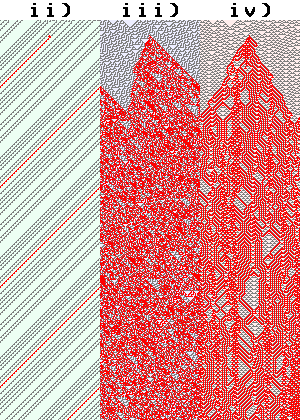
\includegraphics[width=\linewidth]{Images/P4/4classesDiffPatt.png}
    \caption{Difference Pattern in red for Class-$2$, Rule-$6$ (ii); in Class-$3$, Rule-$30$ (iii); and in Class-$4$, Rule-$54$ (iv).}
    \label{fig:4classDiffPatt}
\end{figure}







\clearpage



\begin{figure}
    \centering
    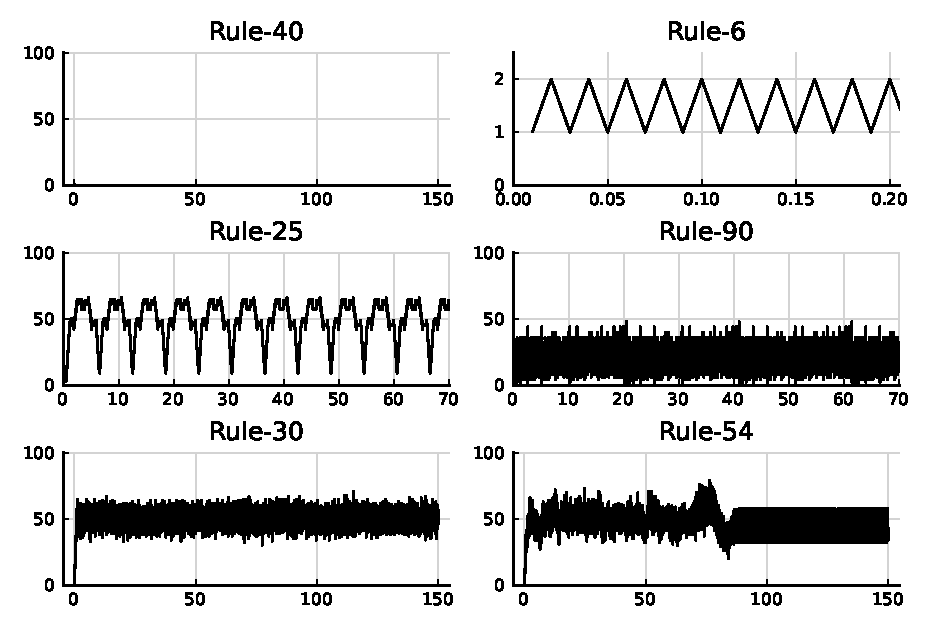
\includegraphics[width=\textwidth]{Images/P4/HammingTimeSeries.eps}
    \caption{For 6 different rules belonging to: Class-$1$ (Rule-$40$), Class-$2$ subclass LP (Rule-$6$), Class-$2$ subclass HP (Rule-$25$), Class-$3$ subclass U (Rule-$90$), Class-$3$ subclass C (Rule-$30$) and Class-$4$ subclass T (Rule-$54$); we represent the Hamming distance over time. The horizontal axis is in units of $L=100$ iterations, which is the size of the population.}
    \label{fig:HammDistTimeSeries}
\end{figure}


\begin{figure}
    \centering
    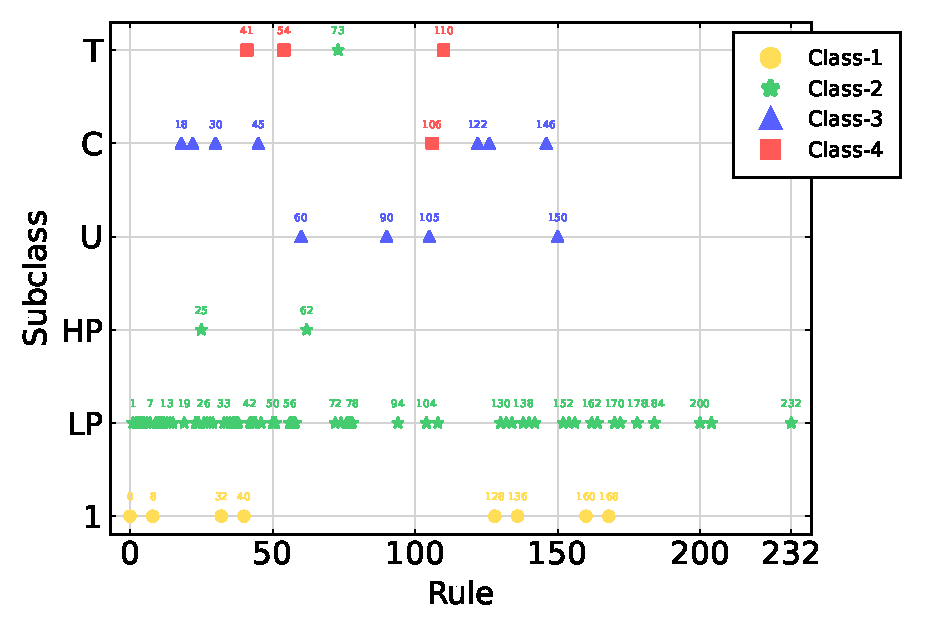
\includegraphics[width=\linewidth]{Images/P4/HammingClass.eps}
    \caption{Hamming distance classification. Colors and symbols correspond to Wolfram's classification, while position at the vertical axis correspond to the subclasses.}
    \label{fig:HammDistClass}
\end{figure}



\section{Hamming distance classification}

A way to observe how susceptible a given rule is to minimal changes in the initial conditions are the difference patterns. Each class has characteristic differences when comparing its difference patterns. As we can see in Fig.~\ref{fig:4classDiffPatt} the difference pattern for Class-$1$ is null, periodic for Class-$2$, noisy for Class-$3$ and complex for Class-$4$. In our study we have focused our attention in the number of cells that are different at each iteration. This is, again, the Hamming distance, which we used in the previous chapter. Here we obtain the Hamming distance of two initially close configurations varying only in one cell versus time, and analyze the saturated time series instead of the growth. 


We show the Hamming distance for $6$ rules that present different behavior in Fig.~\ref{fig:HammDistTimeSeries}. We have grouped together all rules that present the same behavior in a sub-classification of Wolfram's classification. The subclass column in Table~\ref{tab:ECAclasses} and Fig.~\ref{fig:HammDistClass} collects this information. Different initial conditions may produce a time series with different behavior. To help us to asses how complex can a rule get, we have classified the rule taking into account the time series with the most complex behaviour along $100$ different computations.

For Wolfram Class-$1$, the Hamming distance time series at this class goes rapidly to $0$. 

For Class-$2$ the time series varies periodically or is constant. We have subclass LP for low periods of no more than $20$ iterations, though most have period lesser than $5$; and HP for high periods greater or around $5L$ iterations. We can obtain the period o the series through its autocorrelation.

In Class-$3$ we have subclass U and C. Rules in subclass C give chaotic time series. Whereas those in subclass U have exactly the same time series for all initial conditions. The series is periodic, but with an extremely long period of exactly $2046$ iterations. This is very close to a power of $2$, $2^11 = 2048$. In fact with different values of $L$ one obtains that the periods of the Hamming distance are approximate to different powers of $2$. What is more, if the populations size is set to a power of $2$, the Hamming distance goes to $0$ after some iterations. Looking at Fig.~\ref{fig:Rule90}, where we represent the difference pattern for Rule-$90$, which it is the same than the pattern of evolution, we see that the patterns scale and repeat at periods that get multiplied by $2$. This is due to the auto-similarity that charactherizes this patterns as fractal.
As we explain below, all rules in subClass-$U$ are intrinsically fractal.




\begin{figure}
    \centering
    
\includegraphics[width=\linewidth]{Images/P4/Sierpinski.png}
    \caption{Evolution of the ECA Rule-$90$ of size $1024$ starting with a single black cell, i.e. a $1$, at the center. If instead there is a single $0$ at the beginning, it gives the same result except with a black line at the top. This figure matches exactly with the difference pattern between two ECA's of the same rule and size where, after a brief transient (one iteration is enough), the state of the central cell is altered to be a $1$. The ECA forms a fractal named Sierpiński triangle.}
    \label{fig:Rule90}
\end{figure}




Class-$3$ automata evolve to complex patterns, so the fact that all initial conditions produce the same time series, is hard to believe. We can explain it analysing an intrinsic characteristic of these rules. For this explanation we will consider Rule-$90$ and its truth table from Table~\ref{tab:Rule90}. The rest of rules in this subclass have the same explanation. Choose any row from the table. If that row has a $0$ at the right side, then altering any of the trios at the left side of any row by adding modulo $2$ the trio of the row you chose would not alter the result on the right. If instead it had a $1$ at the right, the it would indeed alter the result. The rule itself is fractal. These only happens with rules in subclass U and marks the fractal behaviour of these rules, since, for these rules the evolution of a single $1$ in a sea of $0$s or vice-versa produces a fractal pattern like in Fig.~\ref{fig:Rule90}, that is exactly the same as the difference pattern of the rule with any initial condition.

Finally Class-$4$ is represented by subclass T, in which rules present transient chaos in the Hamming distance time series. The chaotic regime holds while there is complex behavior in the patterns and finishes when the evolution saturates in a periodic state.



\begin{figure}
    \centering
    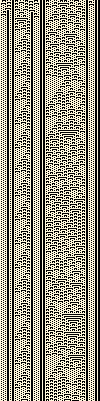
\includegraphics[height=0.95\textheight]{Images/P4/73.png}
    \caption{Time evolution of Rule-$73$ over $400$ iterations. Besides being classified as Class-$2$ in \textit{WolframAlpha}, this patterns belong to Class-$4$ more accurately.}
    \label{fig:Rule73}
\end{figure}





Each subclass belongs to one Wolfram class as appears on \textit{WolframAlpha} except for two rules. This is the case for Rule-$73$, which belongs to Wolfram Class-$2$ but subclass T. The rule was classified in this subclass because in one, and only one, of the $100$ time series we saw transient chaos. In Fig.~\ref{fig:Rule73} we see an evolution pattern that could be classified to Wolfram Class-$4$, but this behaviour happens in rare occasions. Rules in the $HP$ subclass are close to being from subClass-$T$ also, but since the times where the patterns are complex are very narrow, we did not detect transient chaos.

Rule-$106$ is also an exception. We have classified it as subclass C whereas in \textit{WolframAlpha} is classified as Class-$4$. Watching the pattern evolution in Fig.~\ref{fig:Rule106} we clearly see this is an error, as the patterns looks more akin to those in Class-$3$.




\begin{figure}
    \centering
    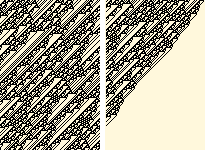
\includegraphics[width=\linewidth]{Images/P4/106.png}
    \caption{Time evolution of Rule-$106$. At the left, the evolution under periodic boundary conditions shows patterns that never repeat for long times like those at Class-$3$. At the right, evolved under a fixed boundary, the zeros propagate to the left until all cells are zero, making it fall under definition of Class-$1$.}
    \label{fig:Rule106}
\end{figure}



\section{Discussion and conclusions}

We have made an algorithm that classifies the ECA rules analyzing a time series instead of analyzing an image. Thus requires less quantity of data to analyze than Wolfram method, so it is more effective. The classification separates the rules in the same classes save for some arguably misclassified rules in the \textit{WolframAlpha} engine. This is not a setback  because Wolfram's classification was subject of variance given different initial conditions.

With the autocorrelation of the Hamming distance we can also obtain its period, but this is not generally the period of the cellular automaton, and has a strong dependence with populations size.


\begin{thebibliography}{04}

\bibitem{PhysicsCA1}
\raggedright
D. Chowdhury, L. Santen, and A. Schadschneider,
Statistical physics of vehicular traffic and some related systems.
Phys. Rep. \textbf{329}, 199--329 (2000).
\url{https://doi.org/10.1016/S0370-1573(99)00117-9}


\bibitem{PhysicsCA2}
\raggedright
C. Burstedde, K. Klauck, A.Schadschneider, and J. Zittartz,
Simulation of pedestrian dynamics using a two-dimensional cellular automaton. 
Physica A \textbf{295}, 507--525 (2001).
\url{https://doi.org/10.1016/S0378-4371(01)00141-8}

\bibitem{PhysicsCA3}
\raggedright
D. H. Rothman and J. M. Keller,
Immiscible cellular-automaton fluids.
J. Stat. Phys. \textbf{52}, 1119--1127 (1988). 
\url{https://doi.org/10.1007/BF01019743}

\bibitem{PhysicsCA4}
\raggedright
L. Kadanoff, S. R. Nagel, L. Wu, and S. Zhou,
Scaling and universality in avalanches.
Phys. Rev. A \textbf{39}, 6524 (1989).
\url{https://doi.org/10.1103/PhysRevA.39.6524}

\bibitem{PhysicsCA5}
\raggedright
D. A. Meyer,
From quantum cellular automata to quantum lattice gases.
J. Stat. Phys. \textbf{85}, 551--574 (1996).
\url{}

\bibitem{EngineeringCA1}
\raggedright
P. Tougaw, L. Douglas, and S. Craig,
Logical devices implemented using quantum cellular automata.
J. Appl. Phys. \textbf{75}, 1818--1825 (1994).
\url{https://doi.org/10.1007/BF02199356}

\bibitem{CryptographyCA1}
\raggedright
S. Nandi, B. K. Kar, and P. Pal Chaudhuri,
Theory and applications of cellular automata in cryptography.
IEEE Trans Comput \textbf{43} 1346--1357 (1994).
\url{https://doi.org/10.1109/12.338094}

\bibitem{CryptographyCA2Lya}
\raggedright
J. Machiacao, A. G. Marco, and O. M. Bruno,
Chaotic encryption method based on life-like cellular automata.
\textbf{39}, 12626--12635 (2012).
\url{https://doi.org/10.1016/j.eswa.2012.05.020}

\bibitem{BiologyCA1}
\raggedright
J. Lechleiter, S. Girard, E. Peralta, and D. Clapham,
Spiral calcium wave propagation and annihilation in Xenopus laevis oocytes.
Science \textbf{252}, 123--126 (1991).
\url{https://doi.org/10.1126/science.2011747}

\bibitem{BiologyCA2}
\raggedright
K. C. De Carvalho and T. Tomé,
Probabilistic cellular automata describing a biological two-species system.
Mod. Phys. Lett. B \textbf{18}, 873--880 (2004).
\url{https://doi.org/10.1142/S0217984904007396}

\bibitem{BiologyCA3}
\raggedright
M. Redeker, A. Adamatzky, and G. J. Martínez,
Expressiveness of elementary cellular automata.
Int J Mod Phys C \textbf{24}, 1350010 (2013).
\url{https://doi.org/10.1142/S0129183113500101}

\bibitem{VonNeummanCA}
\raggedright
J. von Neumann, A. W. Burks, 
Theory of Self-Reproducing Automata. 
University of Illinois Press (1966).
\url{https://cdn.patentlyo.com/media/docs/2012/04/VonNeumann.pdf}

\bibitem{WolframCA_ClassOrigen}
\raggedright
S. Wolfram,
Universality and complexity in cellular automata.
Physica D \textbf{10}, 1--35 (1984).
\url{https://doi.org/10.1016/0167-2789(84)90245-8}

\bibitem{UniversalComputingECA110}
\raggedright
M. Cook,
Universality in Elementary Cellular Automata.
Complex Syst. \textbf{15}, 1--40 (2004). 
\url{https://content.wolfram.com/sites/13/2018/02/15-1-1.pdf}
\end{thebibliography}



\clearemptydoublepage


\chapter{Escaping from transient chaos with partial control} %6P1
\label{chap:ForcingEscape}


\begin{quotation}
	\vspace{-3cm}
    \begin{flushright}
    \begin{minipage}[t][5cm][b]{0.5\textwidth}
    {\letquote ``Fantasy is hardly an escape from reality. It's a way of understanding it."}
    
    \bigskip
    
    -{\small  Lloyd Alexander}
    \end{minipage}
    \end{flushright}
    
    \vspace{0.5cm}
\end{quotation}



\vspace{0.5cm}


\let\thefootnote\relax\footnotetext{
%\bibitem{Alfaro2021}
G. Alfaro, R. Capeáns, and M. A. F. Sanjuán,
Forcing the escape: Partial control of escaping orbits from a
transient chaotic region,
Nonlinear Dyn. \textbf{104}, 1603--1612 (2021).\\
\url{https://doi.org/10.1007/s11071-021-06331-4}
}



\vspace{1cm}



Partial control has been developed as a control method generally used in chaotic transients, where the controller does not fix a given orbit, but instead chooses a set of points to avoid. In this chapter, we introduce this concept to further develop it in the two following chapters, where we use the partial control method to solve a game between two players. 

\section{Introduction}

The partial control method was firstly introduced to solve the Yorke's Game of Survival in~\cite{Yorke'sGame} where a game is defined between a ``protagonist" and an ``antagonist". The goal of the protagonist was to survive in a chaotic transient region indefinitely. In the former paper's case, the region was $[0,1]$ with the slope three tent map $f(x) = \mu(1-|x|)-1$ as the dynamics of the system. The antagonist role was interpreted by the effect of an additive noise, which bound was larger than the control bound of the protagonist.

This map is well known and the iteration of the map in the sequence $x_{i+1} = f(x_i)$ for slopes greater than two, presents transient chaos. This is because the map is only positive for the region $[-1,1]$ and for those slopes, the orbits leave that region after falling near $0.5$ and escape towards $-\infty$. Through the iteration of the map all initial points eventually escape, since only the zero-measure Cantor ternary set remains an indefinite amount of time in the chaotic transient. The escape times depend on the initial conditions and present fractality. Therefore they are highly unpredictable in the disturbed case as can bee seen on Fig.~\ref{fig:EscapeTimes}. Orbits that start near the Cantor set take many iterations to escape without disturbance. Although in Fig.~\ref{fig:EscapeTimes} we used the logistic map, the graphic is similar for the tent map.

Given that all points eventually escape and that the noise bound is greater it is unlikely that the protagonist could survive. However, with the partial control method, it is possible to find sets of points called the safe set for each combination of control bound and noise bound. Given a noise bound and a control bound there is a unique set that enables the protagonist to stay in the region if the initial conditions belongs to the set, for as long as control is active. The sets were firstly found by using the sculpting algorithm~\cite{Sculpting} and later the safe functions were developed which enable to find multiple safe sets for different control bounds more efficiently~\cite{SafeSets}.

But what drives the study presented in this chapter is not to maintain the orbits in the chaotic region, but to take out the unpredictable manner in which orbits escape from the region. We aim to control the orbits in order of being certain to know how the orbits will escape. We will get some functions similar to the safe functions that allows us either to escape from the chaotic transient region in the least iterations possible, or to set the exact number of iterations that passes before the orbits escape. We called these functions the escape functions, and the sets, the escape sets.
 
\section{Escape from a region with partial control}

Given a map $f(x)$, with a bounded additive noise $\xi_n$ that affects the map at each iteration $n$, we eject a bounded additive control $u_n$, which, as we mentioned earlier, can be smaller than the noise bound. We define the iterated map that acts on $q\in Q$, $Q$ being a region in phase space as:

\begin{equation}
\begin{split}
&q_{n+1}=f(q_n)+\xi_n+u_n \\
&|\xi_n|\leq \xi_0 \\
&|u_n|\leq u_0.
\end{split}
\end{equation}

The goal is to find the correct sequence of controls ($u_1$, $u_2$,..., $u_m$) to ensure that at the $m^{th}$ iteration, with $m \leq N$, the point $q_{m+1}$ is outside of the region $Q$. $N$ is the maximum number of iterations it will take to achieve the goal, but in some cases, depending on the initial condition, the orbit can be expelled sooner. When setting a very small $N$, the control bound should be high, or otherwise achieving the goal may not be possible. On the other hand, by setting a large $N$ the control bound can be smaller and smaller.

To apply this control technique one should firstly choose the region $Q$ from where the orbits must escape. Then one should compute $N$ quick escape functions $U_k$, $k = 1:N$, which depend on the value $\xi_0$. These functions tell how much control is needed to expel the orbit in $k$ iterations or less.

Then, by setting the control bound $u_0$ compute the escape sets $E_k$ for every escape function. Every point which belongs to this set can be thrown out from the region $Q$ in $k$ or fewer iterations. Each escape set contains all the points which have a value of $U_k$ lower than $u_0$. Since $E_N$ may not gather every point in the region $Q$, if the orbit starts in one of those point that are not gathered in $E_N$, the escape is not guaranteed to be made in $N$ iterations, and could take larger times.

Now, when all escape sets are computed, the control strategy is to push the point $f(q_i) + \xi_i$ towards the escape set with the lower index $k$ that is within control reach.

We also developed a similar algorithm to make the escape from the region $Q$ in an orderly manner, i.e., to escape in exactly $N$ iterations, no more, no less. The procedure is the same as we have explained above, except that the escape functions are different and for the control strategy we have to push the first point towards $E_N$, the second iteration towards $E_{N-1}$ and so on, until the controlled orbit gets to $E_1$ after which the application of the map, noise, and control, the point is outside region $Q$.

Finally we presented a practical case in which we shift the trajectory from one chaotic region to another periodically, resulting in a quasiperiodic orbit.

\section{Application of the method}

To give an example on how to apply the algorithms, we have chosen the logistic function $f(x) = \mu x(1-x)$. For $\mu > 4$ there is a chaotic transient on the region $Q=[0,1]$. 

\begin{figure}
    \centering
    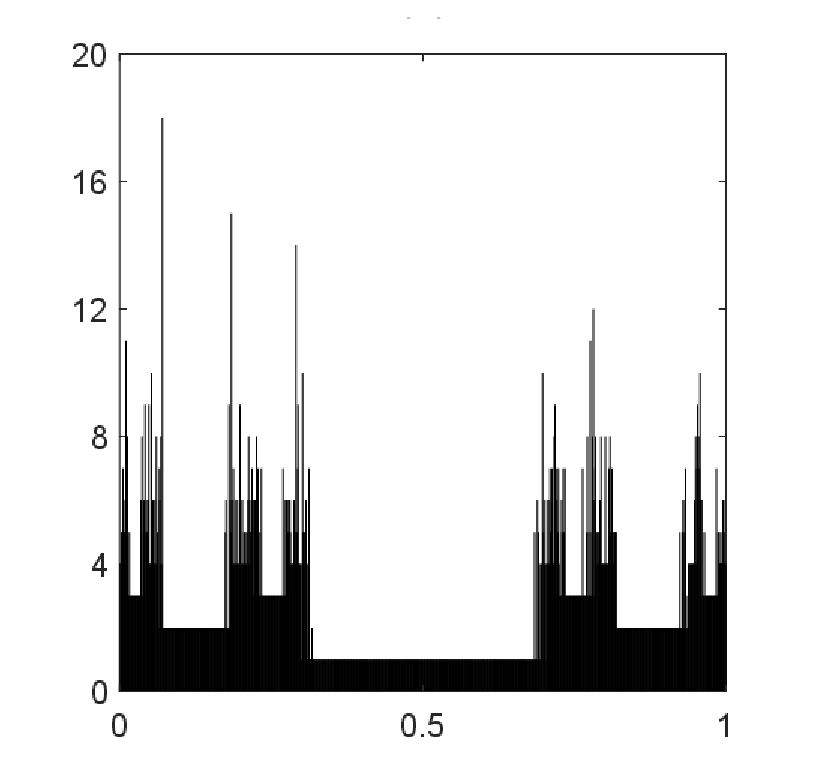
\includegraphics[width=0.5\linewidth]{Images/P1/EscapeTimes.eps}
    \caption{Escape times from the chaotic transient of the logistic map with $\mu=4.7$ and a noisy disturbance bounded to $\xi_0 = 0.03$. Horizontal axis represents the starting points for the orbit and the vertical axis, the number of iterations of a random orbit before it escaped the chaotic transient region $Q = [0,1]$.}
    \label{fig:EscapeTimes}
\end{figure}

In the following subsections we present the algorithms to calculate the escape functions and sets in order to achieve three distinct goals. First, to make the orbits escape region $Q$ as quickly as possible setting a maximum number of iterations $N$. Next, to set an exact number of iterations $N$ after which the orbit must be outside region $Q$. Finally, to make a quasiperiodic orbit that shifts between two chaotic transients at fixed intervals $N_1$ and $N_2$ iterations. 

\subsection{Escaping as quick as possible}

We want to make orbits to escape in $N$ iterations or less. The larger the control bound is, the quicker some orbits will escape and the escape sets will be broader. This will be helpful if one wishes to avoid as much as possible chaotic orbits which can be dangerous in some situations. The authors of~\cite{AvoidTransient1} state that ``transient chaos may be a dangerous and unwanted state of a vibro-impact system". 

Since we are making numerical calculations, we must use a grid on region $Q$. We divide the region in $M$ equal parts, so that the region transforms in a collection of equidistant points $q[i]$, $i=1:M$. Also the value of the noise is discretized into $W$ values ranging from $-\xi_0$ to $\xi_0$. The map then becomes:

\begin{equation}
    q[j] = f(q[i]) +\xi[s] +u[i,s,j],
\end{equation}
where $q[j]$ is the arrival point with $j=1:M$. Now we are ready to compute the escape functions.

Firstly we compute the escape function $U_1$. This function tells us the control necessary for every point in the region $Q$ to escape in the next iteration. 
\begin{equation}
U_1(q[i]) = \max\limits_{s}(\min(f(q[i]) + \xi[s] + \epsilon - 0, 1 + \epsilon - (f(q[i]) + \xi[s]))),
\end{equation}
where $0$ and $1$ are the limits of the region $Q$ and $\epsilon$ is a small number to ensure the escape and is convenient to be $1/M$.

If $f(q[i]) + \xi[s]$ is beyond $Q$ then change the function value to $0$, since there is no need for control.

Then, we calculate the following functions recursively with this formula:

\begin{equation*}
u[i,s,j] = q[j] - f(q[i]) - \xi[s]
\end{equation*}
\begin{equation*}
U^{*}_{k+1}[i]=\max_s\Big(\min_j\big(\max(|u[i,s,j]|,U_k[j])\big)\Big)
\end{equation*}
\begin{equation}
U_{k+1}[i]=\min\bigg(U_k[i],U^{*}_{k+1}[i]\bigg),
\label{equ:QuickEscapeFunctions}
\end{equation}
where $u[i,s,j]$ is the control to take the resulting point, after the application of the map and noise, to each point in the grid. The last equation ensures that the escape can be done in less than $N$ iterations.

\begin{figure}
    \centering
    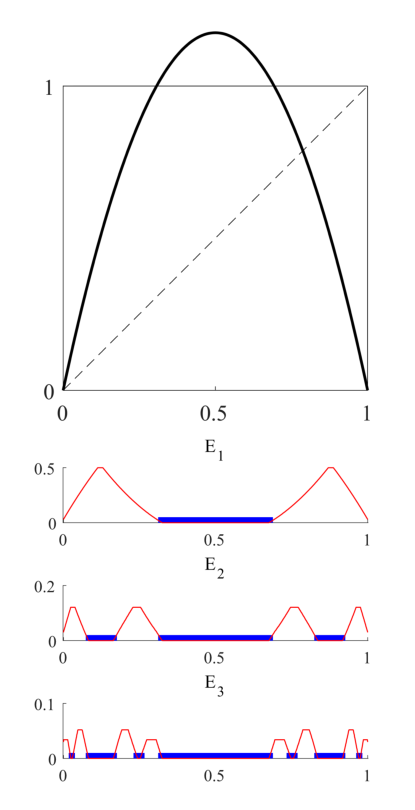
\includegraphics[width=0.4\textheight]{Images/P1/EscapeSetsQuick.eps}
    \caption{On top, logistic map $\mu x(1-x)$ with $\mu = 4.7$. On the bottom, escape functions (red) and escape sets (blue) for escaping in $N=3$ or less iterations as quick as possible. The functions were computed for a noise bound of $\xi_0 = 0.03$ and the sets for a control bound of $u_0 = 0.022$. The vertical axis shows the minimum control needed for orbits starting at each starting point to stay in the chaotic transient region $Q = [0,1]$ indefinitely, which mark the quick escape functions in red. The quick escape sets $E_k$ are highlighted in blue and their heights are trivial. The points in these sets can be controlled with the given control bound to escape in at maximum $i$ iterations.   }
    \label{fig:EscapeSetsQuick}
\end{figure}

We give an example with $N=3$ in Fig.~\ref{fig:EscapeSetsQuick}. The escape sets in blue are the regions of the escape functions in red that have lower value than the control bound. Each index $k$ in $E_k$ tells in how many iterations is possible to escape. 

Now in order to escape as quick as possible, the controller must push the iterated point of the orbit towards the lowest indexed escape set reachable. 

By increasing the number of iterations we allow for the orbit to escape $N$, the escape sets will become larger. For $N\to\infty$ the set becomes the entire region except the zero-measure Cantor ternary set. This will not be the case for the following case in which the orbit must escape at an exact number of iterations.


\subsection{Escaping at an exact number of iterations}

Now we ask ourselves if it is possible to set the exact number of iterations before an orbit is expelled from the chaotic transient. This seems a difficult task when considered the restriction of limiting control to be smaller than noise, since some points naturally escape in one iteration, while others take a lot of time to do so. 

However, we repeat the same line of work as the previous case, by constructing the exact escape functions and later by getting the exact escape sets. When inspecting the logistic map, points at the center will escape naturally in the next iteration, so probably these points won't be in the exact escape sets for large values of their index. On the other hand points near the Cantor ternary set seem to be out of bounds for the sets with small index. This landscape will be reflected on the exact escape functions which are constructed differently than in the previous case.

In spite of the task seeming harder, the algorithm to calculate the escape functions is very similar and even simpler. $U_1$ is calculated the same obviously. Then the rest of the functions are computed exactly as equations~\ref{equ:QuickEscapeFunctions} but without the last equation. In this case, we do not check whether the function is smaller than the function with lower index since we cannot allow for an earlier escape.

\begin{equation*}
u[i,s,j] = q[j] - f(q[i]) - \xi[s]
\end{equation*}
\begin{equation}
U_{k+1}[i]=\max_s\Big(\min_j\big(\max(|u[i,s,j]|,U_k[j])\big)\Big)
\label{equ:ExactEscapeFunctions}
\end{equation}





\begin{figure}
    \centering
    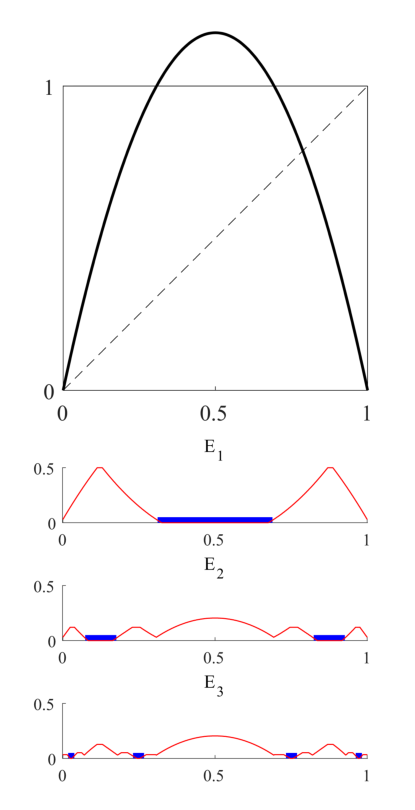
\includegraphics[width=0.4\textheight]{Images/P1/EscapeSetsExact.eps}
    \caption{On top, logistic map $\mu x(1-x)$ with $\mu = 4.7$. On the bottom, escape functions (red) and escape sets (blue) for escaping in $N=3$ or less iterations as quick as possible. The functions were computed for a noise bound of $\xi_0 = 0.03$ and the sets for a control bound of $u_0 = 0.022$. The vertical axis shows the minimum control needed for orbits starting at each starting point to stay in the chaotic transient region $Q = [0,1]$ indefinitely. The blue lines mark the exact escape sets $E_k$, their heights are meaningless, the points in $E_k$ can escape in exactly $k$ iterations with the given control bound. }
    \label{fig:EscapeSetsExact}
\end{figure}




Following this formula, we arrive to the exact escape functions and sets in Fig.~\ref{fig:EscapeSetsExact}. We can see that the sets are smaller, because the set $E_k$ doesn't contain the contents of $E_{k-1}$, unlike the previous case. Each exact escape set $E_k$ is the complementary of the $k-th$ approximate Cantor ternary set $C_k$, though a little bit decreased or increased depending on whether the noise is greater than the control or vice versa. 

Now, to escape in exactly $N$ iterations, we must simply take the first iterated point towards $E_{N-1}$. This will be possible only if the initial point started in $E_N$. Afterwards we will push the iterated point one escape set further at a time until $E_1$ is reached. Then, after iterating the map the orbit will be out of the chaotic region or the border will be within reach of control.




\subsection{Shifting chaotic transients}



\begin{figure}
    \centering
    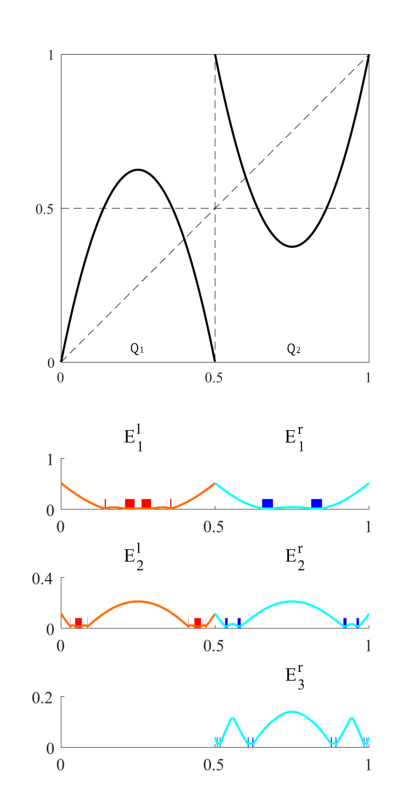
\includegraphics[width=0.4\textheight]{Images/P1/Alt_sets.eps}
    \caption{On top, the custom made double parabola map for $\mu = 10$. It present two differentiated zones at left and right of the middle point at $0.5$. At the bottom we present the shift functions as lines and sets as blocks. The shift fucntions $U^{l,r}_k$ tells how much control is needed at least to keep the orbit in the left or right region for $k$ iterations before shifting to the other region. In this case we have calculated the functions and sets in order to keep the orbit $N^l = 2$ iterations at the left and $N^r = 3$ iterations to the right.}
    \label{fig:ShiftSets}
\end{figure}



\begin{figure}
	\centering
	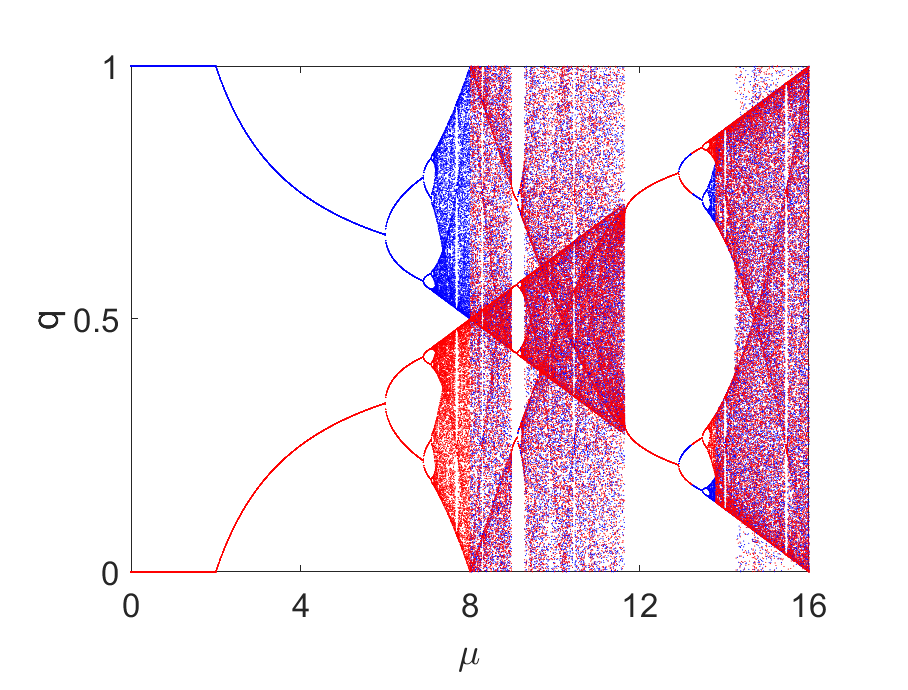
\includegraphics[width=1\linewidth]{Images/P1/Alt_Bifurcation.eps}
	\caption{Bifurcation diagram for the double parabola map choosing two different initial conditions. Te points in red correspond to starting the trajectories in $Q_l$ and when in blue, the trajectories started in $Q_r$. For $\mu>8$ a global atractor merges and both regions are accessible to the trajectories.} 
	\label{fig:Alt_Bifurcation}
\end{figure}


\begin{figure}
	\centering
	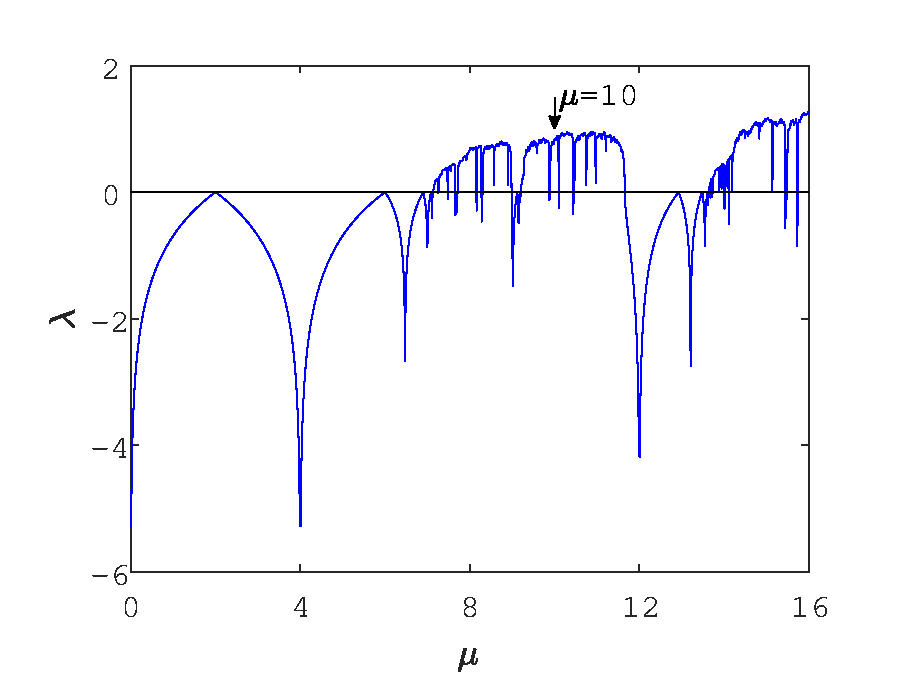
\includegraphics[width=1\linewidth]{Images/P1/Alt_Lyapunov.eps}
	\caption{Evolution of the Lyapunov exponent versus $\mu$ for the double parabola map. For positive values of the exponent, the dynamics are chaotic.}
	\label{fig:Alt_Lyapunov}
\end{figure}




\begin{figure}
    \centering
    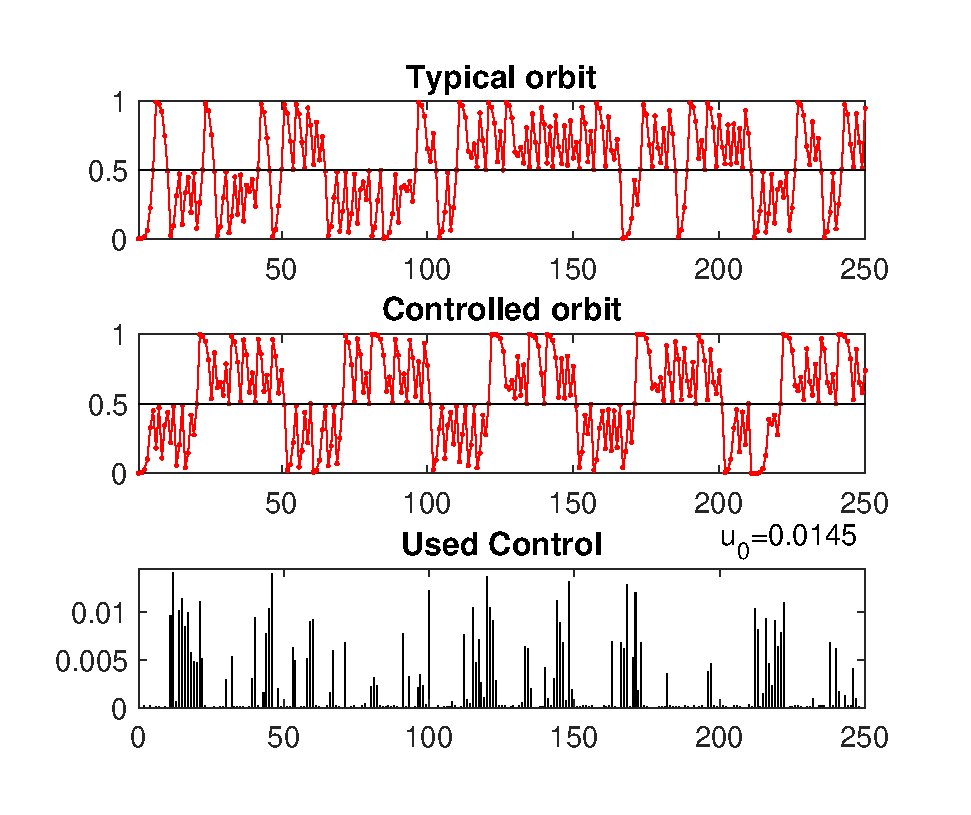
\includegraphics[width=0.7\textheight]{Images/P1/Alt_tray_mu8.1.eps}
    \caption{Controlled and uncontrolled orbits of the double parabola map for $\mu = 8.1$ in red. The typical orbit describes the motion of a chaotic system where the attractor has different regions. The orbits stay an indefinite amount on each side of the attractor shifting chaotically. This is typical of a multistable chaotic system in the moment when its different attractors have merged into a larger one. We were able to control the dynamics in the map so it keeps the chaotic behavior in each side of the attractor, but have controlled the frequency of the shifts. As we can see the controlled orbits spends $N^l = 20$ iterations at the left side and $N^r = 30$ at the right one. The control made at each iteration was at most the value of its bound $u_0 = 0.0145$ which is lower than the noise bound $\xi_0 = 0.015$}
    \label{fig:TrajectoryDouble}
\end{figure}

 

Thanks to the previous control method we can accurately control the escape from a chaotic transient in an orderly manner. This can be helpful in a case where a rigorous control of time is needed. This next case goes forward in this direction, by setting the frequencies of time at which a controlled orbit shifts from one chaotic transient to another. With this control technique one can build a chaotic clock in which a desired chaotic system changes significantly at some desired rates and still maintaining its chaotic behavior. 

This can be useful in multistable chaotic systems. In these kind of systems, varying a parameter one can merge various atractors into a larger one with different regions when their basin boundary collides. The orbit shifts chaotically from one region to the other continuously~\cite{Multistable2}. One example of this motion is the Lorentz system~\cite{Lorentz}, and others are given in~\cite{Multistable2, Multistable3, Multistable4}.

With the following control method, one could make this shifts to appear periodically as long as control is made while maintaining the chaotic motion through the rest of the orbit. The orbit will therefore be quasi-periodical.

We will develop this method on a simple model to show the procedure. On the top graphic of Fig.~\ref{fig:ShiftSets} we show the custom made double parabola map:

\begin{equation}
f(x) = \left\{ \begin{array}{ll}
-\mu (x^2 - \dfrac{1}{2}x)  & \mbox{if $x<0.5$,} \\
1 + \mu (x^2 -\dfrac{3}{2}x + \dfrac{1}{2})  & \mbox{if $x\geq 0.5$,} 
\end{array}
\right.
\end{equation}


The bifurcation diagram and Lyapunov exponent for the iterated map $x_{n+1} = f(x_n)$ are shown in Figures \ref{fig:Alt_Bifurcation} and \ref{fig:Alt_Bifurcation} respectively. It shows that there is a chaotic behavior for most values of $\mu \geq 7.14$ and for values of $ 7.14 \leq \mu < 8$ there are two separated atractors that merge at $\mu = 8$ into a larger one. Then, for values close to that, the orbit shifts chaotically between the left and right regions. 

Figure~\ref{fig:TrajectoryDouble} shows one typical orbit and the controlled one. The uncontrolled trajectory is characterized by chaotic shifts from the left region to the right one, while the controlled trajectory results in a quasi-periodic signal with periodic shifts between the two regions. Also, we can see that the magnitude of the control made at each iteration is no more than a certain bound, which is lower than the noise bound.



To control this orbits we have used the same approach as the previous cases. In this case through the shift functions and sets. which are similar than the escape sets. This time we have to take into account how to stay in a region and how to leave from it and go to the other. So, we need to calculate the control $u_{in}^{l,r}$ as the control needed to get an iterated point in region $Q^{l,r}$ to another desired point in the same region.
\begin{equation*}
u_{in}^{l,r}[i,s,j] =  q^{l,r}[j] - f(q^{l,r}[i]) - \xi[s].
\end{equation*}
And to change regions, the control $u_{out}^{l,r}$ tells the distance between one point from region $Q^{l,r}$ to another from the opposite region $Q^{r,l}$.
\begin{equation*}
u_{out}^{l,r}[i,s,j] = q^{r,l}[j] - f(q^{l,r}[i]) - \xi[s].
\end{equation*}



\begin{algorithm}[h!]
    \caption{Iterative process to calculate the shift functions $U^{l,r}_{k}$ to stay in the left or right side of the double parabola map a number of iterations $N^l$ and $N^r$ respectively.} 
    \label{alg:ShiftFunction}
\renewcommand{\thealgorithm}{}
\floatname{algorithm}{}

\begin{algorithmic}[0]
    \While{$U^{l,r}_{k}$ \text{are different than previous iteration}} 
    
        \For{$k=1:N^l-1$}

          \State  $U^{l}_{k+1}(q[i])=\max\limits_s\Big(\min\limits_j\big(\max(u_{in}^l[i,s,j],U^l_k(q[j]))\big)\Big)$

        \EndFor
    
       \State   $U^{r}_{1}(q[i])=\max\limits_s\Big(\min\limits_j\big(\max(u_{out}^r[i,s,j],U^l_{N^l}(q[j]))\big)\Big)$   
        
        \For{$k=1:N^r-1$}
        
            \State  $U^{r}_{k+1}(q[i])=\max\limits_s\Big(\min\limits_j\big(\max(u_{in}^r[i,s,j],U^r_kq([j]))\big)\Big)$
            
        \EndFor
        
        \State  $U^{l}_{1}(q[i])=\max\limits_s\Big(\min\limits_j\big(\max(u_{out}^l[i,s,j],U^r_{N^r}q([j]))\big)\Big)$
    \EndWhile
    \end{algorithmic}
\end{algorithm}









Taking as a seed $U^l_1 = 0$,  we can calculate the shift functions $U^{l,r}_k$ following Algorithm~\ref{alg:ShiftFunction}. This algorithm calculates the amount needed to control the orbit $k$ iterations at the left, or right, region before shifting to the other region. The shift sets $E^{l,r}_k$ will be the set of points that have a lower value of the function than their bound of control. The sets $E^{l,r}_k$ are ordered like the exact escape sets from previous section, with the index $k$ indicating the number of iterations needed until the orbit will shift to the other region. 

An example is given in Fig.~\ref{fig:ShiftSets}. We calculated the shift sets in order for the orbit to remain $N^l = 3$ at the left side, and $N^r = 2$ at the right side. Following the example, if an orbit starts at a point in $E^l_3$ it will arrive at $E^l_2$ and then $E^l_1$ through control after which, it can be controlled to shift to $E^r_2$, then repeating the same process on the right side until the orbit can be shifted to the left. This process can be continued indefinitely. If one is fortunate and the orbit starts at a point with low value of the shift function, the control can be made lower than the noise.


\section{Discussion and conclusions}

We have applied the partial control method with the goal of driving off trajectories from a chaotic transient region. We developed two methods of doing this. Firstly the controller may want to expel the trajectory as swift as possible. Alternatively, the control can be made in an orderly manner, choosing the exact number of iterations that the trajectory stays at the transient region from the beginning of control to the moment the trajectory leaves the region.

Another case was studied in which the controller shifts periodically between two regions of a multistable chaotic system. In these kind of systems the trajectory shift in chaotic manner from one region to the other, but with the control method provided here, we controlled the frequency of these shifts. The result is a quasi-periodic orbit in which there is a periodical shifting through the two regions, but the orbit inside each region remains chaotic.

The control method does not provide a given orbit to follow strictly, but instead analyses the system and finds sets of points reachable within control limits that serve to complete the goal. The controller can then choose from those points, whether randomly or with other priorities in mind, where to direct the orbit. The outstanding fact about this control method is that there are occasions in which the maximum control can be set to be lesser than a known noise bound.

A simple example is given for each of the three cases. The logistic map was studied in the first two cases and for the control of a multistable system, we crafted a custom made map consisting of two disjointed parabolas with opposite convexity.

For all the cases we managed to achieve the goal at some set of initial conditions even when control was lesser than noise. Increasing the control ensures that more initial conditions are able to be controlled.



\begin{thebibliography}{05}

\bibitem{Yorke'sGame}
J. Aguirre, F. d’Ovidio, and M. A. F. Sanjuán
Controlling chaotic transients: Yorke’s game of survival
Phys. Rev. E \textbf{69}, 016203 
(2004).
\url{https://doi.org/10.1103/PhysRevE.69.016203}

\bibitem{Sculpting}
J. Sabuco, S. Zambrano, M. A. F. Sanjuán, and J. A. Yorke,
Finding safety in partially controllable chaotic systems.
Commun Nonlinear Sci Numer Simulat \textbf{17}, 4274–4280 
(2012).
\url{https://doi.org/10.1016/j.cnsns.2012.02.033}

\bibitem{SafeSets}
R. Capeáns, J. Sabuco, M. A. F. Sanjuán,
A new approach of the partial control method in chaotic
systems.
Nonlinear Dyn. \textbf{98}, 873–887 
(2019). 
\url{https://doi.org/10.1007/s11071-019-05215-y}



\bibitem{AvoidTransient1}
V.A. Bazhenov, O. S. Pogorelova, and T.G. Postnikova,
Transient chaos in platform-vibrator with shock.
Strength Mater. Theory Struct. \textbf{106}, 22-40 
(2021).
\url{https://doi.org/10.32347/2410-2547.2021.106.22-40}

\bibitem{Multistable1}
Y.~F. Jin,
{\em Stochastic resonance in an under-damped bistable system driven by harmonic mixing signal}, 
Chinese Phys. B \textbf{27}, 050501 
(2018).
\url{https://doi.org/10.1088/1674-1056/27/5/050501}

\bibitem{Lorentz}
E. N. Lorenz,
Deterministic nonperiodic flow.
J. Atmos. Sci. \textbf{20}, 130-141 
(1963).
\url{https://doi.org/10.1175/1520-0469(1963)020<0130:DNF>2.0.CO;2}


\bibitem{Multistable2}
E.~L. Rempel and A.~C.-L. Chian, 
{\em Intermittency induced by attractor-merging crisis in the Kuramoto-Sivashinsky equation}, 
Phys. Rev. E \textbf{71}, 016203 
(2005).
\url{https://doi.org/10.1103/PhysRevE.71.016203}

\bibitem{Multistable3}
A.~L. Livorati, I.~L. Caldas, C.~P. Dettmann, and E.~D. Leonel,
{\em Crises in a dissipative bouncing ball model},
Phys. Lett. A \textbf{379}, 2830--2838 
(2015).
\url{https://doi.org/10.1016/j.physleta.2015.09.016}

\bibitem{Multistable4}
S.~Vaidyanathan, S.~T. Kingni, A.~Sambas, M.~A. Mohamed, and M.~Mamat,
{\em A new chaotic jerk system with three nonlinearities and synchronization via adaptive backstepping control},
Int. J. Eng. Technol. \textbf{7}, 1936--1943 
(2018).
\url{https://doi.org/10.14419/ijet.v7i3.15378
}



\end{thebibliography}
\clearemptydoublepage


\chapter{Two-Player Yorke's Game of Survival in Chaotic Transients} %7P5
\label{chap:PartialControlGame}

In the previous chapter we developed a method of partial control that followed the line of work initiated in \cite{Yorke} followed by papers on the issue \cite{DynamicsPartialControl,PartialControlBeyond,PartialControlFunctions} among others. The study led to the publication of \cite{PartialControlEscape}. 

The problem introduced in \cite{Yorke} was devised as a kind of game where one player is at a huge disadvantage but, nonetheless, can achieve its goal. From there on the studies derived in a control method that did not force a single trajectory as the solution, but provided a set of points, the \textit{safe sets}, where the controller was safe; hence the name \textit{partial control}.

On the other hand, game theory provides powerful tools for analyzing strategic interactions across diverse fields, from social sciences to economics and physics \cite{Social,EconomyGames,GamesComplex}. While classical game theory typically focuses on equilibrium states, many real-world situations involve chaotic systems, where extreme sensitivity to initial conditions and inherent unpredictability create fundamental challenges for strategic decision-making. The nonlinear nature of these systems makes traditional game-theoretic approaches insufficient, as small perturbations can lead to dramatically different outcomes. What's more, the intrinsic characteristics of a game are susceptible to change in real life, and these changes can result from the players' decisions \cite{AkiyamaKaneko1,AkiyamaKaneko2}.

Game theory has also proven valuable in chaos control \cite{GamesControl}, where control problems naturally emerge as competitive scenarios between opposing objectives. This framework reveals how controllers must optimize their strategies while dealing with three key challenges: (1) the unpredictable nature of chaotic dynamics, (2) the system constraints, and (3) the actions of other controllers who must carefully choose their actions to achieve their own goal. This interaction between different control agents adds a strategic dimension that goes beyond traditional chaos control methods.

Since this thesis is oriented towards game dynamics, the opportunity to rejoin this two branches of the problem led to the publication of \cite{PartialControlGame}. In this paper we present a two-player game of control where each player has conflicting objectives. One player wants to control the trajectory of a given dynamical system towards one region and the opponent towards a different one. Through the analysis of the game with the partial control tools we achieve the solution of the game through all initial conditions. We will construct the \textit{winning sets} (what was previously called \textit{safe sets}), as the initial conditions that guarantee victory for each player.

To illustrate the game we studied a paradigmatic dynamical system, the logistic map ${f(x) = \mu x_n(1-x_n)}$. The system presents transient chaotic dynamics for $\mu>4$ where all orbits starting at the region $Q=[0,1]$ eventually leave the region in a finite time. When one player aims to stay at the region $Q$ indefinitely and the other aims to drive the trajectory off, the game gets very interesting. In one hand, the game is asymmetric since the player who wants to leave region $Q$ is in advantage. On the other hand, we found that there are initial conditions where the player that aims to conserve the trajectory in the transient region can do so even when their control is lesser than the opponent's control.

In many games the order of play is important. This game is no exception, here the importance lies in the information that the second player has when they see the action of the opponent. Knowing where the opponent is going to push the trajectory to will affect the decision of control of the second player, giving them an advantage that the first player lacks. To study this effect, we devised three scenarios. In the first game the player that aims to keep the trajectory in the region $Q$ knows the action of the rival. In the second one, the informed player is the one who intends to expel the trajectory form the region. Finally, in the third game, no player knows the rival's action. The lack of knowledge in this last game will translate in the unsettled solution of the game. Regions where no player has the victory assured appear as a consequence of these lack of knowledge.


\section{The game}


\begin{figure}
    \centering
    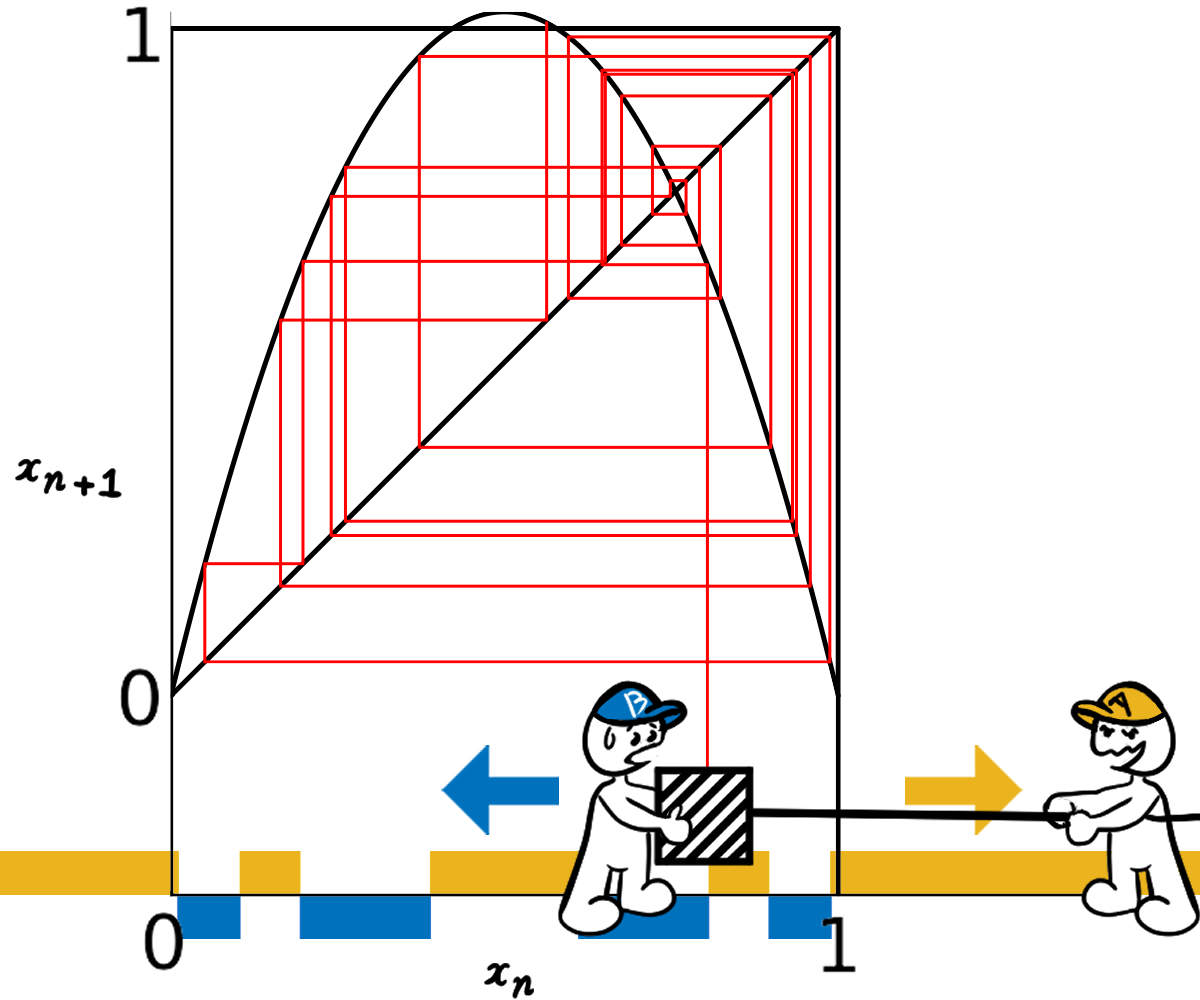
\includegraphics[width=0.7\textwidth]{Images/P5/drawing.png}
    \caption{Players $A$ and $B$ compete for controlling the trajectory on the chaotic and escaping logistic map $x_{n+1} = \mu x_n(1-x_n)$. Player $B$ tries to maintain the trajectory on the region $Q = [0,1]$, while fighting against the dynamics of the map, since for $\mu > 4$ all points except a zero measure Cantor set eventually escape from the region. The red line shows an example of one orbit that ends up escaping. Furthermore, player $B$ also fights against the opponent, player $A$, who aims to expel the trajectory from region $Q$ in a finite time. To achieve their goals the players can control the trajectory with a given control bound. The yellow and blue rectangles are the \textit{winning sets} of players $A$ and $B$, respectively. These are the initial conditions that guarantee victory for each player.}
    \label{fig:drawing}
\end{figure}





Considers two persons pulling an object. Player A wants to pull it to their side, while Player B
pulls toward their own. With no other factor present, the stronger player will
win by pulling harder. However, the game becomes much more interesting when the object naturally moves
described by a rule given by a function $f$. Now, the players have to consider the force of the rival at the same time than the object's natural movement. This becomes especially difficult when the object's movement described by $f$ is chaotic, meaning that even tiny changes in how they pull can lead to completely different and unpredictable results, as is illustrated in Fig.~\ref{fig:drawing}.

Formally, we describe the game as follows. Consider a region $Q$ of the phase space where a map $f$ acts on the state space $X$. The initial state $x$ of the game starts in $Q$. Player $B$'s objective is to keep the trajectory within $Q$, while player $A$ aims to drive the trajectory outside of $Q$. Each iteration of the game consists of players $A$ and $B$ choosing their respective bounded controls $u_n^A$ and $u_n^B$.  At each discrete time step $n$, the state $x_n$ evolves according to this dynamics
\begin{equation}
    x_{n+1} = f(x_n) + u_n^A + u_n^B,
\end{equation}
where $u_n^A $ and $u_n^B $ represent the control actions of players $A$ and $B$, respectively. These controls are bounded by
\begin{equation}
    |u_n^A| \leq u_0^A, \quad |u_n^B| \leq u_0^B.
\end{equation}


Player $B$ needs to maintain the trajectory inside $Q$ forever to win, while $A$ only needs to drive the trajectory outside $Q$ once to achieve victory.

A critical aspect to solve this game is the order of play. For this reason, we consider three different scenarios:
\begin{table}[h!]
\centering
\begin{tabular}{|p{3cm}|p{4cm}|p{7.3cm}|}
\hline
\textbf{Game Type} & \textbf{Order of Play} & \textbf{Information Available} \\
\hline
Game $A^{-}B^{+}$ & $B$ plays after $A$ & B knows $A$'s action  \\
\hline
Game $A^{+}B^{-}$ & $A$ plays after $B$ & $A$ knows $B$'s action  \\
\hline
Game $A^{-}B^{-}$ & Simultaneous play & Both ignore the opponent's action  \\
\hline
\end{tabular}
\caption{Three different scenarios analyzed in this paper based on the order of play, i.e., what information is available to each player.}
\label{tab:games}
\end{table}



In game $A^{-}B^{+}$, player $B$ has the advantage of knowing player $A$'s action before making their move. This sequential play allows $B$ to react optimally to $A$'s choice. In game $A^{+}B^{-}$, the roles are reversed, with $A$ having complete information about $B$'s move before acting. Finally, in game $A^{-}B^{-}$, both players must make their decisions simultaneously, where both players ignore the action of their opponent.










\section{Solving the game: The winning sets}




\begin{figure}[h!]
    \centering
    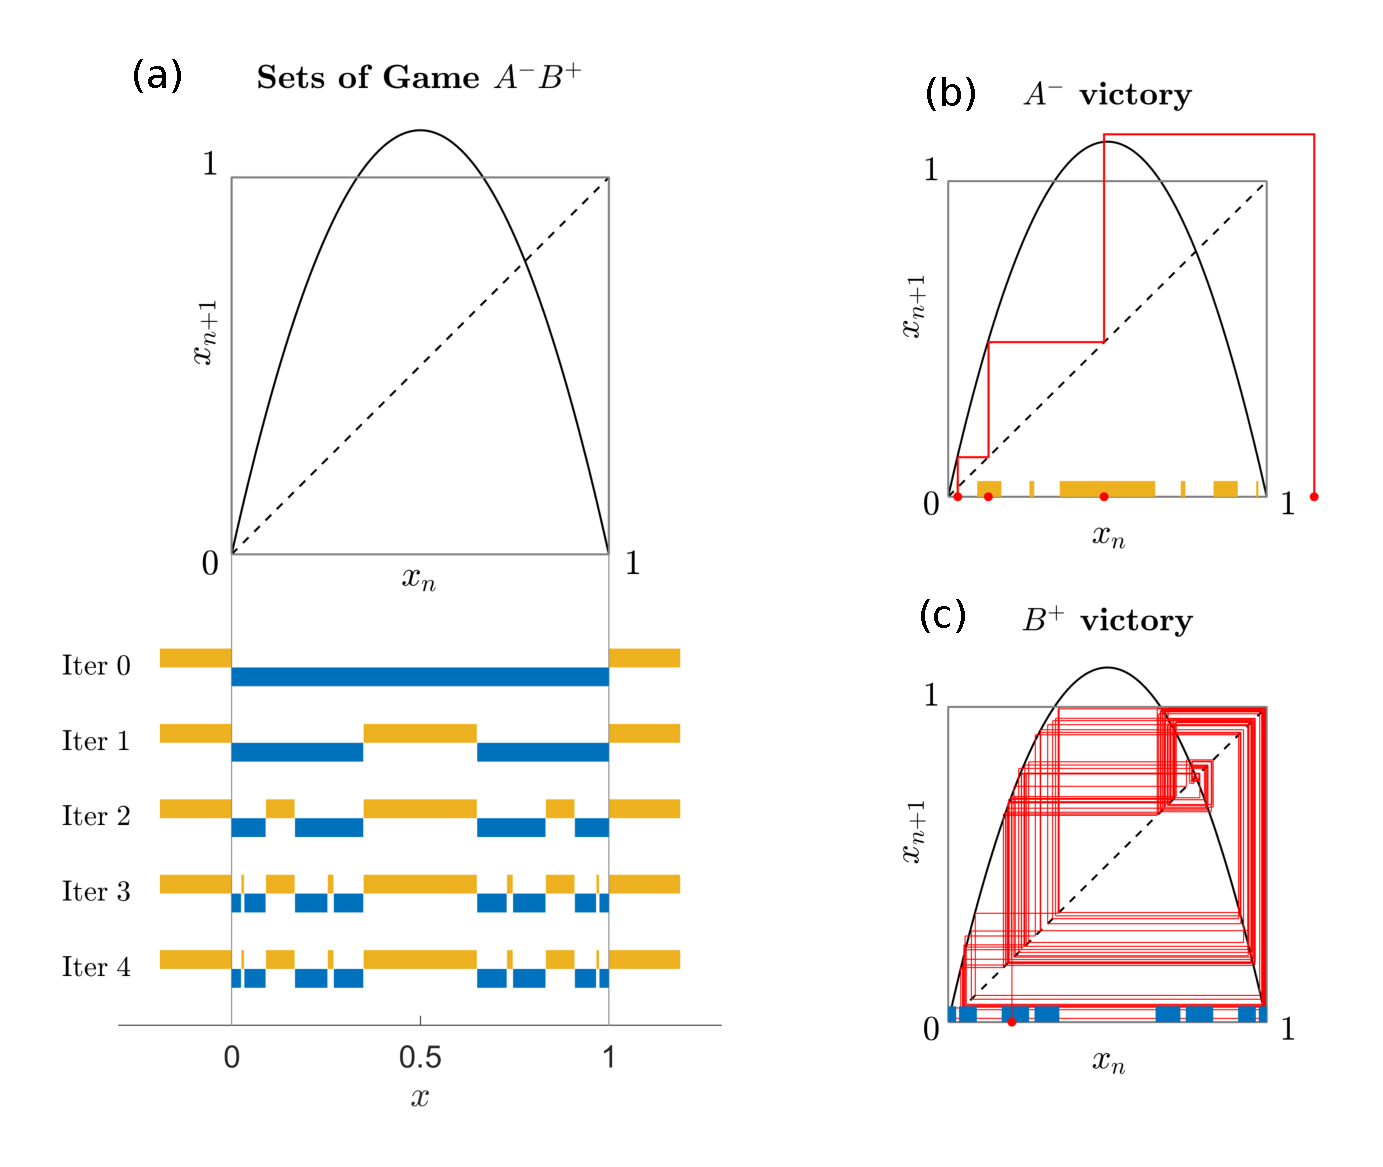
\includegraphics[trim={0.8cm 0cm 0cm 0cm}, clip,width=0.95\textwidth ]{Images/P5/setsAB_control.eps}
    \caption{ Winning sets and controlled trajectory for a game between an ignorant player $A$ and an informed player $B$. (a) Steps of the algorithm to compute the winning sets for the ignorant player $A$, $W^{A^-}$, in yellow, and for the informed player $B$, $W^{B^+}$, in blue. The sets were computed in the region $R\in [-0.3,1.3]$, with $Q\in[0,1]$, $u_0^A=0.016$, $u_0^B=0.038$. The algorithm converges in $3$ iterations since  the sets for the third iteration are identical to those of the forth. (b) Controlled trajectory of the game when the initial condition belongs to player's $A$ winning set. Player $A$ acts first, without knowledge of player $B$'s move, so they choose its control at each step to reach the closest point belonging to the shrunk set ($W^{A^-} -u^B_0$), accounting for the worst possible subsequent action of player $B$. After $3$ iterations the trajectory has left region $Q$, so player $A$ wins. (c) The game now starts in a point that belongs to player's $B$ winning set. Player $B$ acts second, with the knowledge of player $A$'s move, so selects their control to reach the closest point belonging to set $W^{B^+}$. The trajectory stays indefinitely inside region $Q$, so player $B$ wins as long as control is maintained.}
    \label{fig:tray}
\end{figure}



\begin{figure}[h!]
    \centering
   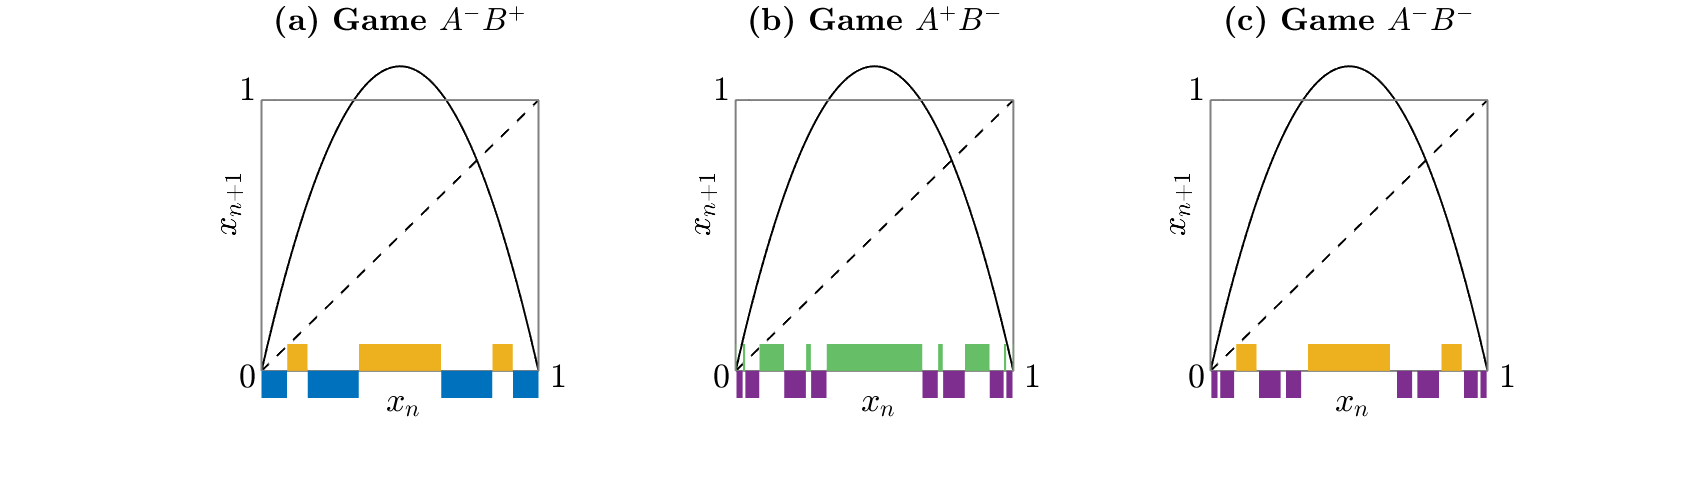
\includegraphics[trim={3.2cm 0cm 0cm 0cm}, clip,width=1.1\textwidth ]{Images/P5/sets_juego.png}
    \caption{The logistic map and winning sets to control trajectories of the logistic map with $\mu = 4.5$ and control bounds $u^A_0 = 0.015$ for player $A$, and $u^B_0 = 0.040$ for player $B$. Each winning set at the bottom show the initial conditions that guarantee victory to each player. Each player has two winning sets whether they are informed ($+$) or ignorant ($-$) to their opponent's move. The winning sets of player $A$ are colored in green when they are informed and in yellow when they are ignorant. On the other hand, those of player $B$ are colored in blue when they are informed and purple when they are ignorant. For simplicity, we only represent the winning sets in the interval $Q$. (a) Ignorant player $A$ against informed player $B$ (b) Now the informed player is $A$ who plays against the ignorant player $B$ (c) Neither player knows each other actions. In this case, there are regions that do not belong to any player's winning set, meaning that both player could win when starting at those initial conditions, but the victory is uncertain because players cannot guarantee victory against any move from the opponent. These "no winning regions" represent the difference between the respective informed winning sets and the ignorant winning sets.}
    \label{fig::sets}
\end{figure}







Given the opposing objectives where player $A$ aims to drive trajectories outside $Q$ while player $B$ seeks to keep them within $Q$, we establish a region $R$ containing $Q$ where the winning sets $W$ are defined for both players. These sets have binary values representing whether that initial condition guarantees victory, $1$, or does not, $0$. For player $B$, initially $W^B(x)=1$ for $x \in Q$ and $0$ otherwise. For player $A$, initially $W^A(x)=0$ for $x \in Q$ and $1$ otherwise. The computation procedure for each winning set is described next, which is also summarized in Table~\ref{tab:morphological_operations}. Each set for an ignorant or informed player $A$ or $B$ can be computed independently.

\begin{itemize}
\item {\bf Player $A^-$ (ignorant player $A$):}
To compute the set of $W^{A^-}$, we have to evaluate for each $x \in Q$ the image $f(x)+u^A+u_0^B$ for all possible controls $u^A \in [-u_0^A,u_0^A]$ and $u^B \in [-u_0^B,u_0^B]$. We select only those $u^A$ where all possible images $f(x)+u^A+[-u_0^B,u_0^B]$ fall within $W^{A^-}$. Points $x \in Q$ satisfying this condition update $W^{A^-}(x)=1$. All these initial conditions are able to be controlled to escape after one iteration of the map. But there will be other points that, after more than one iterations of the map and control, will be able to escape. To find this points we must repeat the algorithm, thus updating $W^{A^-}$ until it converges.

This process is equivalent to iteratively performing the following morphological operations: first shrinking $W^{A^-}$ by $u_0^B$, then dilating by $u_0^A$. For any $x \in Q$ whose $f(x)$ falls within the shrunk set, we set $W^{A^-}(x)=1$. The process is repeated with this new $W^{A^-}$ until it converges.

\item {\bf Player $A^+$ (informed player $A$):}
To compute the set of $W^{A^+}$, we analyze $f(x)+u^B+u^A$ for all possible controls. For each $x \in Q$, we evaluate $f(x)+[-u_0^B,u_0^B]+u^A$ and determine if there exists some $u^A \in [-u_0^A,u_0^A]$ capable of forcing escape for all possible images. If such $u^A$ exists, then $W^{A^+}(x)=1$. This process is performed for all $x \in Q$, updating the set $W^{A^+}$. The algorithm is repeated until $W^{A^+}$ converges.

Morphologically, this process is equivalent to first dilating $W^{A^+}$ with $u_0^A$ and then shrinking the resulting set with $u_0^B$. For any $x \in Q$ whose $f(x)$ falls within this shrunk set, we set $W^{A^+}(x)=1$.

\item {\bf Player $B^-$ (ignorant player $B$):}
To compute the set of $W^{B^-}$, we evaluate for each $x \in Q$ the image $f(x)+u^B+u_0^A$ for all possible controls $u^B \in [-u_0^B,u_0^B]$ and $u^A \in [-u_0^A,u_0^A]$. We select only those $u^B$ where all possible images $f(x)+u^B+[-u_0^A,u_0^A]$ fall within $W^{B^-}$. Points $x \in Q$ not satisfying this condition update $W^{B^-}(x)=0$. Since player $B$ wants to keep the orbit in $Q$ forever, the algorithm must be repeated until $W^{B^-}$ converges.

The process is equivalent to iteratively performing the following morphological operations: first shrinking $W^{B^-}$ by $u_0^A$, then dilating by $u_0^B$. For any $x \in Q$ whose $f(x)$ falls outside the shrunk set, we set $W^{B^-}(x)=0$. The process is repeated with this new $W^{B^-}$ until it converges.

\item {\bf Player $B^+$ (informed player $B$):}
To compute the set of $W^{B^+}$, we analyze $f(x)+u^A+u^B$ for all possible controls. For each $x \in Q$, we evaluate $f(x)+[-u_0^A,u_0^A]+u^B$ and determine if there exists some $u^B \in [-u_0^B,u_0^B]$ capable of guaranteeing containment for all possible images. If such $u^B$ does not exist, then $W^{B^+}(x)=0$. This process is performed for all $x \in Q$, updating the set $W^{B^+}$. The algorithm is repeated until $W^{B^+}$ converges.

Morphologically, this process is equivalent to first dilating $W^{B^+}$ with $u_0^B$ and then shrinking the resulting set with $u_0^A$. For any $x \in Q$ whose $f(x)$ falls outside this shrunk set, we set $W^{B^+}(x)=0$.
\end{itemize}




\begin{table}[h]
\centering
\begin{tabular}{|c|c|>{\raggedright\arraybackslash}p{9.5cm}|}
\hline
Player & Initial Set & \multicolumn{1}{c|}{Morphological Operations} \\
\hline
$A^-$ & 
$\begin{array}{l} 
W^{A^-}(x)=\begin{cases} 
0 & x \in Q \\
1 & \text{otherwise}
\end{cases} \\
\\
W^{A^-}_{\text{new}}=W^{A^-}
\end{array}$ 
& $\begin{array}{l} \\ 
1. \text{ Shrink } W^{A^-} \text{ by } u_0^B \text{ to obtain } W^{A^-}_{\text{shrunk}} \\ 2. \text{ Dilate } W^{A^-}_{\text{shrunk}} \text{ by } u_0^A \text{ to obtain } W^{A^-}_{\text{dilated}} \\ 3. \text{~} \forall x \in Q, \text{ if } f(x) \text{ falls in } W^{A^-}_{\text{dilated}},\text{ set }W^{A^-}_{\text{new}}(x)=1 \\  4. \text{~} W^{A^-}=W^{A^-}_{\text{new}}. \text{ Go to step 1 and repeat the process} \\ ~
\end{array}$ \\ \hline
$A^+$ & $\begin{array}{l}
W^{A^+}(x)=\begin{cases}
0 & x \in Q \\
1 & \text{otherwise}
\end{cases} \\
\\
W^{A^+}_{\text{new}}=W^{A^+}
\end{array}$ 
& $\begin{array}{l} \\ 
1. \text{ Dilate } W^{A^+} \text{ by } u_0^A \text{ to obtain } W^{A^+}_{\text{dilated}} \\ 2. \text{ Shrink } W^{A^+}_{\text{dilated}} \text{ by } u_0^B \text{ to obtain } W^{A^+}_{\text{shrunk}} \\ 3. \text{~} \forall x \in Q, \text{ if } f(x) \text{ falls in } W^{A^+}_{\text{shrunk}},\text{ set }W^{A^+}_{\text{new}}(x)=1 \\  4. \text{~} W^{A^+}=W^{A^+}_{\text{new}}. \text{ Go to step 1 and repeat the process} \\ ~
\end{array}$ \\ \hline
$B^-$ & $\begin{array}{l}
W^{B^-}(x)=\begin{cases}
1 & x \in Q \\
0 & \text{otherwise}
\end{cases} \\
\\
W^{B^-}_{\text{new}}=W^{B^-}
\end{array}$ 
& $\begin{array}{l} \\ 
1. \text{ Shrink } W^{B^-} \text{ by } u_0^A \text{ to obtain } W^{B^-}_{\text{shrunk}} \\ 2. \text{ Dilate } W^{B^-}_{\text{shrunk}} \text{ by } u_0^B \text{ to obtain } W^{B^-}_{\text{dilated}} \\ 3. \text{~} \forall x \in Q, \text{ if } f(x) \text{ falls in } W^{B^-}_{\text{dilated}},\text{ set }W^{B^-}_{\text{new}}(x)=1 \\  4. \text{~} W^{B^-}=W^{B^-}_{\text{new}}. \text{ Go to step 1 and repeat the process} \\ ~
\end{array}$ \\ \hline
$B^+$ & $\begin{array}{l}
W^{B^+}(x)=\begin{cases}
1 & x \in Q \\
0 & \text{otherwise}
\end{cases} \\
\\
W^{B^+}_{\text{new}}=W^{B^+}
\end{array}$ 
& $\begin{array}{l} \\ 
1. \text{ Dilate } W^{B^+} \text{ by } u_0^B \text{ to obtain } W^{B^+}_{\text{dilated}} \\ 2. \text{ Shrink } W^{A^+}_{\text{dilated}} \text{ by } u_0^A \text{ to obtain } W^{B^+}_{\text{shrunk}} \\ 3. \text{~} \forall x \in Q, \text{ if } f(x) \text{ falls in } W^{B^+}_{\text{shrunk}},\text{ set }W^{B^+}_{\text{new}}(x)=1 \\  4. \text{~} W^{B^+}=W^{B^+}_{\text{new}}. \text{ Go to step 1 and repeat the process} \\ ~
\end{array}$ \\ \hline
\end{tabular}
\caption{Morphological operations for each player's winning set computation.}
\label{tab:morphological_operations}
\end{table}







\section{Game of survival in the logistic map}



To illustrate our approach, we study a game based on the logistic map ${f(x) = \mu x_n(1-x_n)}$ where $\mu=4.5$ and $Q=[0,1]$. This map serves as an excellent test case since it exhibits transient chaos in $Q$: trajectories display chaotic behavior before naturally escaping the region. This creates an asymmetric scenario where the player $B$, who wants to stay in the region, must work against both the natural dynamics and their opponent's actions, who has an opposite objective, i.e., to expel the trajectory from the region. While this specific example is used, our methodology can be applied to others maps $f$ and defined regions $Q$ in phase space.

In this context, both players can apply control at each iteration to influence the trajectory, but they are limited by their respective control bounds $u_0^A$ and $u_0^B$. The state of the system at each iteration is determined by
\begin{equation}
x_{k+1} = f(x_k) + u^A + u^B,
\end{equation}
where $f(x) = \mu x(1-x)$ is the logistic map, and $u^A$ and $u^B$ represent the control inputs applied at each iteration according to each player's strategy.






We compute an example for this game with specific control bounds $u_0^A = 0.016$ and $u_0^B = 0.038$. In Fig.~\ref{fig:tray}, we show how the winning sets are constructed. Each iteration of the process brings the winning sets closer to their final version by cutting down player's $B$ set and expanding that of player $A$. Additionally, we show two controlled trajectories with initial conditions belonging to the winning set of player $A$ in Fig.~\ref{fig:tray}(b), successfully expelling the trajectory from region $Q$; and of player $B$ in Fig.~\ref{fig:tray}(c), keeping the orbit in the region. 

Figure~\ref{fig::sets} shows three games whether each player is informed or ignorant, showing the winning sets of each player. In Fig.~\ref{fig::sets}(a), we analyze the case where $A$ plays first and $B$ second. In Fig.~\ref{fig::sets}(b), the roles are reversed: $B$ plays and $A$ plays second. Finally, Fig.~\ref{fig::sets}(c) shows the scenario where both players are ignorant, which could represent a simultaneous play situation.

Particularly interesting is the case shown in Fig.~\ref{fig::sets}(c), where both players play simultaneously and therefore they are ignorant to each other actions. Here, we observe regions in the state space that do not belong to any winning set. These regions emerge because no player can guarantee victory without considering the strategy of the rival. The existence of such regions is a direct consequence of both players being ignorant, no one knows the other player's move when making their decision. Therefore, players may or may not choose the best response to the opponent's move so the outcome depends on the specific combination of controls chosen by both players

This uncertainty contrasts sharply with the scenarios where at least one player is informed, as shown in Fig.~\ref{fig::sets}(a-b), where the winning sets completely determine the game's outcome for all initial conditions.


\subsection{Exploring possible games in the $(u_0^B,u_0^A)$ space}

\begin{figure}
    \centering
    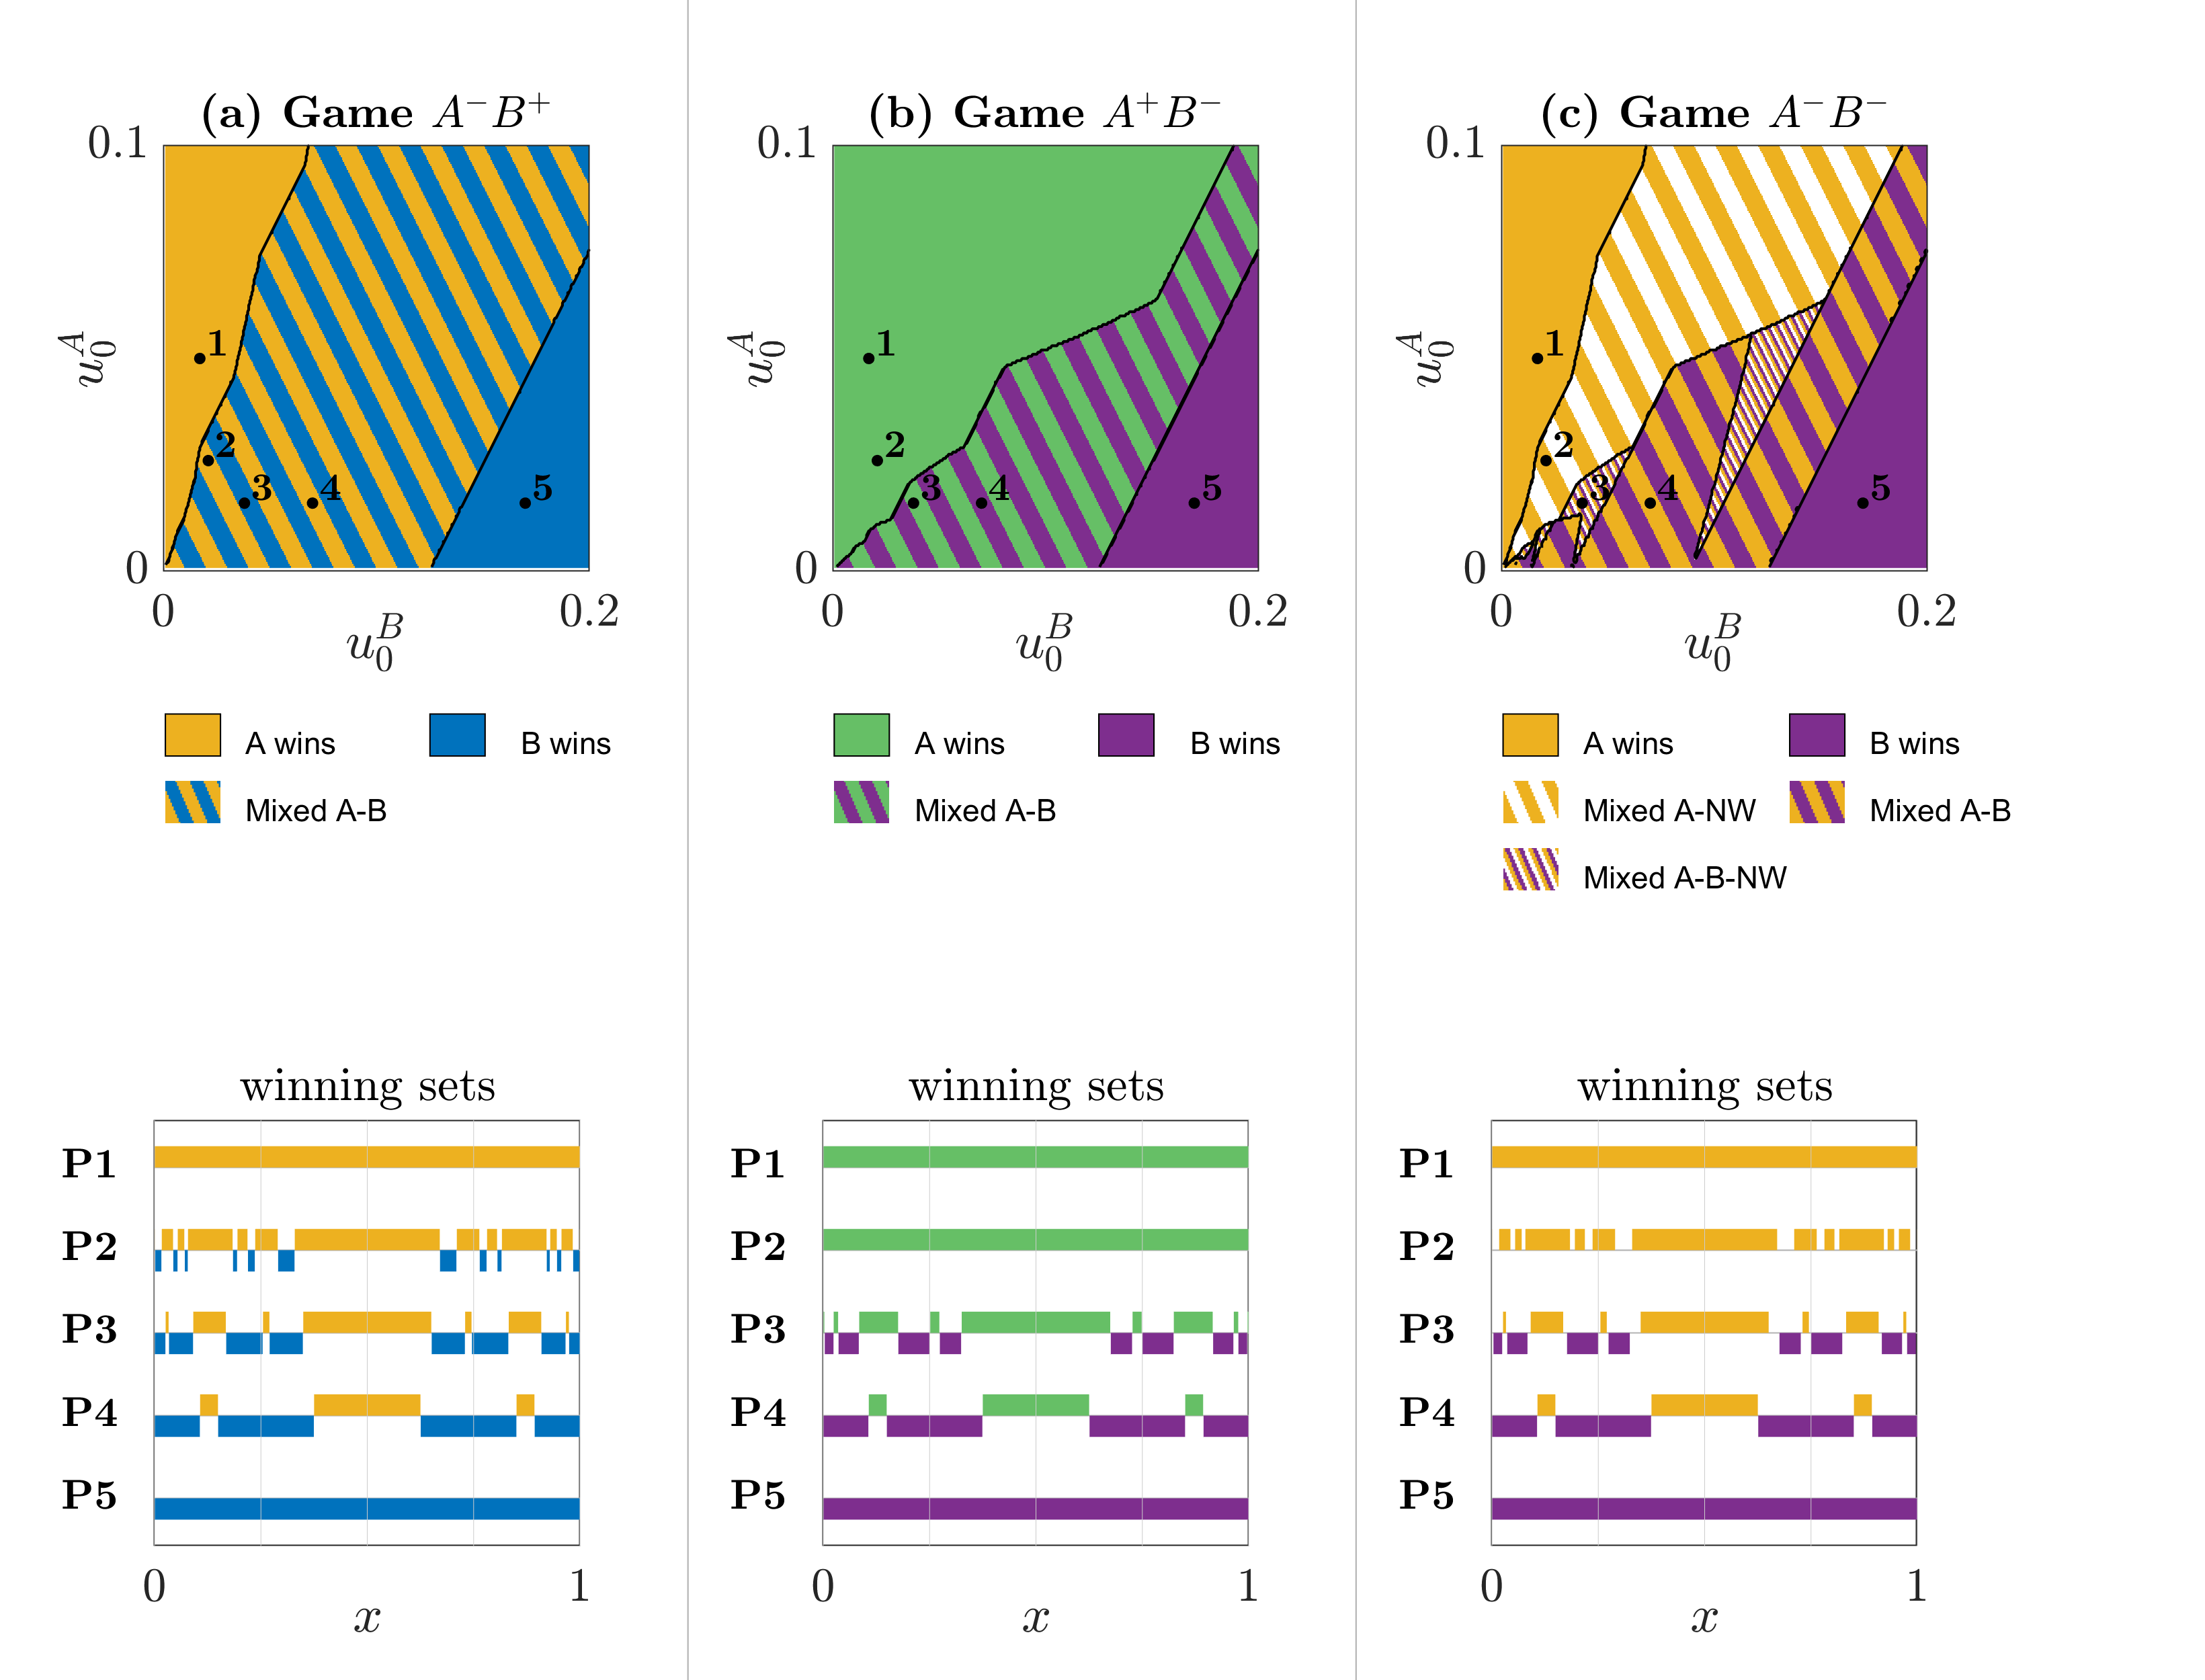
\includegraphics[trim={0.6cm 0cm 0cm 0cm}, clip,width=1.12\textwidth ]{Images/P5/franjas5.png}
    \caption{Different solutions depending on the values of $u^A_0$ and $u^B_0$. Panels (a), (b), and (c) show a diagram in which solid colored regions represent parameter combinations where the informed/ignorant player $A$ wins for all initial conditions at solid colors green/yellow and the informed/ignorant player $B$ at solid blue/purple. Striped regions indicate parameters where the winner depends on the initial conditions. There are also regions with white strips marked as $NW$ (no winning), where the victory is uncertain at some initial conditions. Below each diagram we show the winning sets, i.e., the initial conditions that guarantee victory for each players, for each kind of game at $5$ different regions of control bound. These points, written as $(u^B_0, u^A_0)$, are: $P1 =  (0.017, 0.050)$, $P2 =  (0.021, 0.026)$, $P3 =  (0.038, 0.016)$, $P4=  (0.070, 0.016)$, and $P5= (0.170, 0.016)$. 
    }
    \label{fig:franjas}
\end{figure}


\begin{figure}
    \centering
    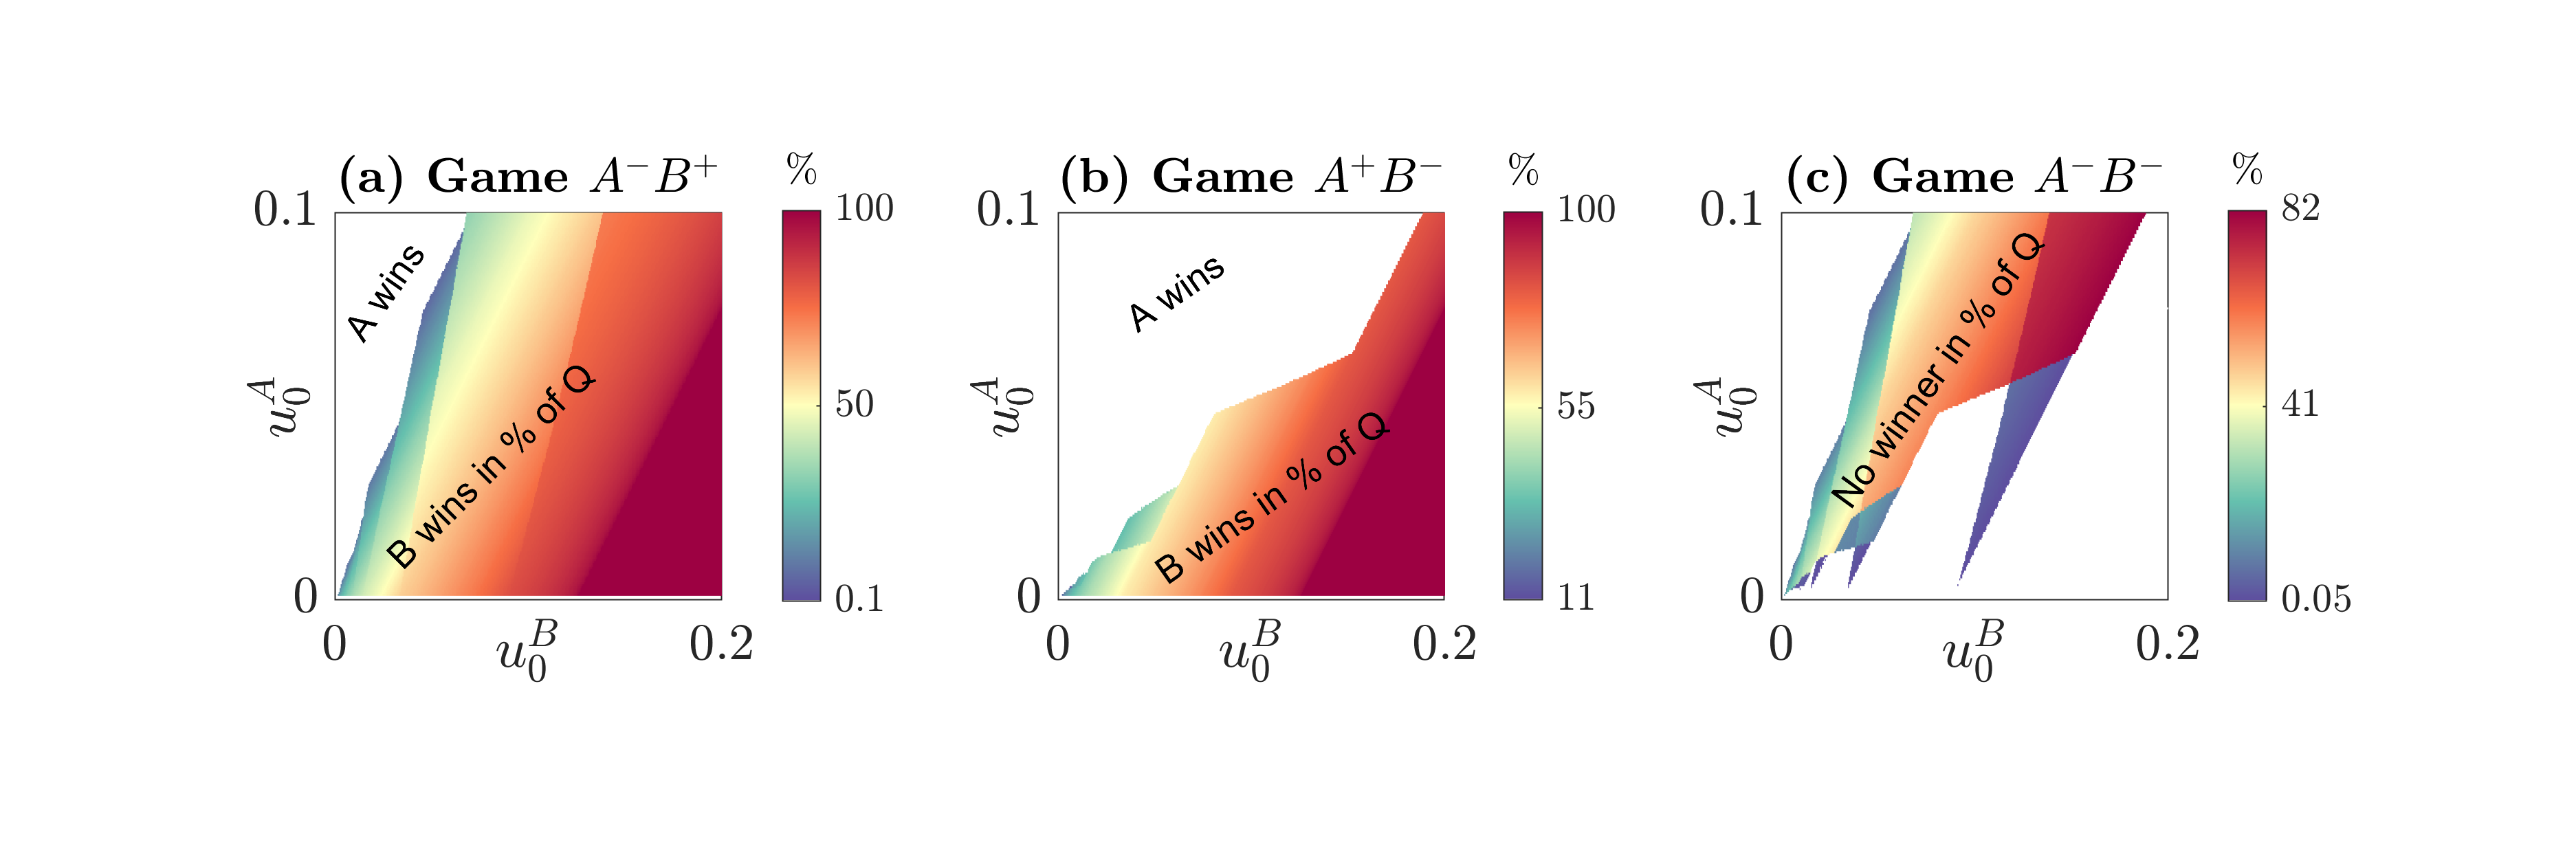
\includegraphics[trim={3.1cm 0cm 0cm 0cm}, clip,width=1.12\textwidth  ]{Images/P5/fraccion.png}
    \caption{The first two panels show the percentage of the region that occupies the winning set of player $B$ respect region $Q$ whether they are informed (+) or ignorant (-). The color is white when the percentage is zero. The last panel represents the percentage of initial conditions that do not assure a winner when both players are ignorant. All figures show similar details at different scales, suggesting self similarity in the system dynamics.}
    \label{fig:fraccion}
\end{figure}

The outcome of these games strongly depends on the control bounds available to each player. Figure~\ref{fig:franjas} presents a comprehensive analysis of possible game scenarios in the $(u_0^B,u_0^A) \in [0,0.2]\times[0,0.1]$ parameter space. It shows three different game types: $A$ ignorant vs $B$ informed, $A$ informed vs $B$ ignorant, and both players ignorant.

In these diagrams, there are regions where one player wins for all initial conditions and other regions in which the winner depends on the initial conditions. Among this last category, in the case where both players are ignorant in Fig.~\ref{fig:franjas}(c), some are marked as $NW$ (no winning) where victory is uncertain for some initial conditions. Five different regions can be seen in Fig.~\ref{fig:franjas}(c). This variety of outcomes illustrates the complexity that emerges when both players must act without knowledge of their opponent's moves.

The bottom Figs.~\ref{fig:franjas}(d-f) illustrate specific examples of winning sets for five different parameter combinations, labeled as games $P1$ to $P5$. These examples demonstrate how the winning sets change as we move through different regions in the parameter space.

Figure~\ref{fig:fraccion} quantifies these results by showing the percentage of region $Q$ occupied by each player's winning set. Particularly interesting is Fig.~\ref{fig:fraccion}(c), which shows the percentage of initial conditions where no player can guarantee victory in the case where both players are ignorant. The color gradients reveal a continuous transition between different game outcomes as the control bounds change.

These results demonstrate how the relative strength of the players' control bounds determines not just who wins, but whether victory can be guaranteed at all. When the bounds are comparable, we often find situations where the outcome depends on initial conditions or remains uncertain.


\subsection{Boundary games}

\begin{figure}
    \centering
    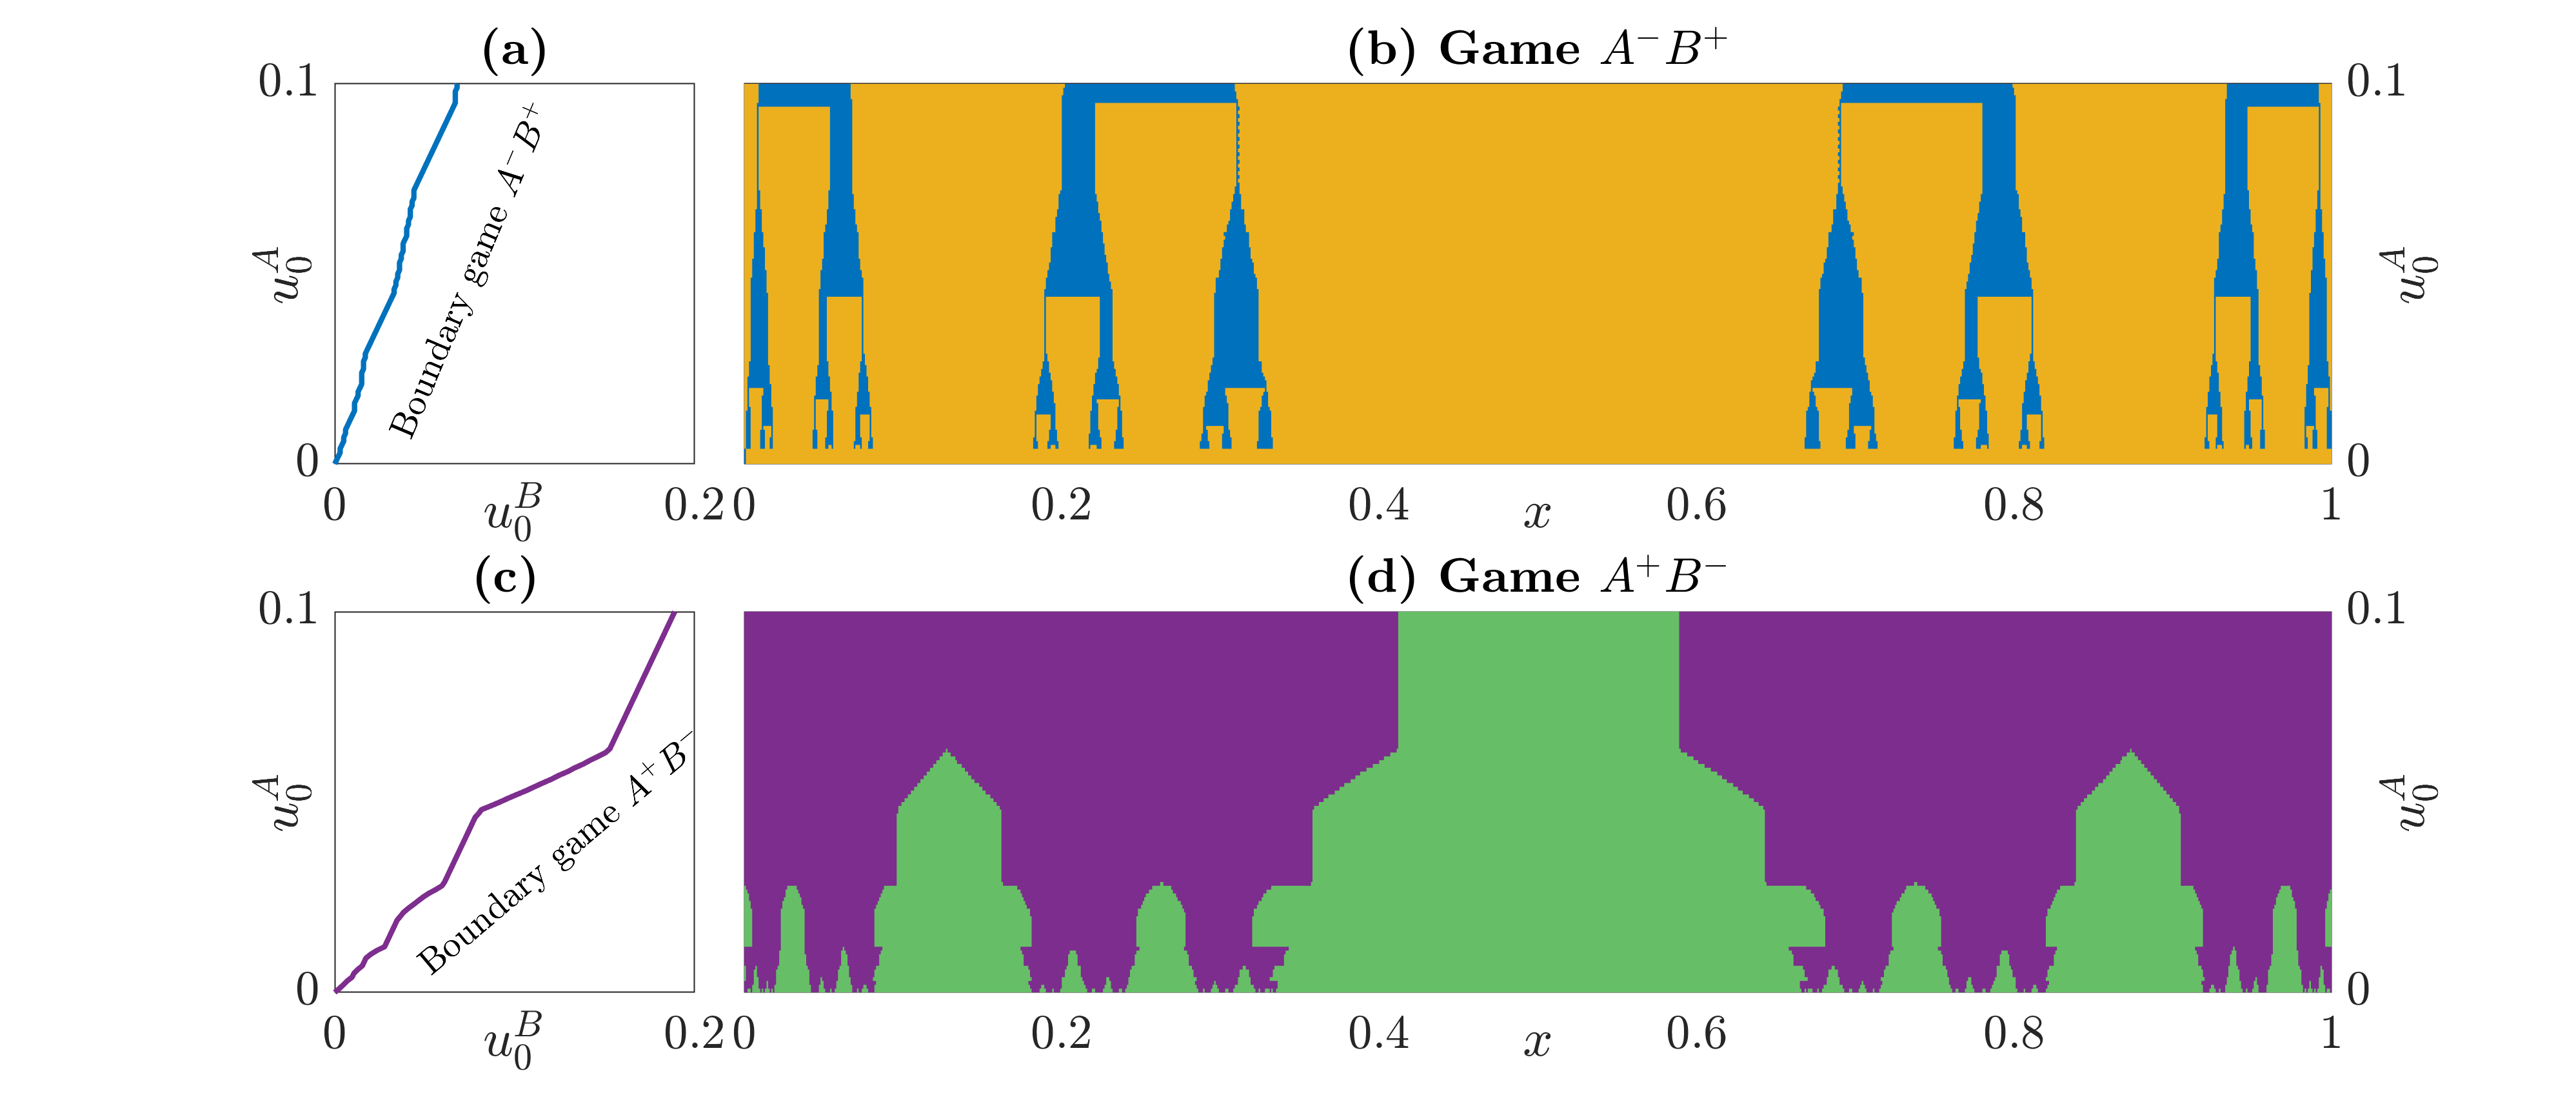
\includegraphics[trim={3.3cm 0cm 0cm 0cm}, clip,width=1.06\textwidth ]{Images/P5/bifurcation.png}
    \caption{Panels (a) and (c) show the game boundary for which there is a shift between player $A$ winning the game at all initial conditions (left of the line) and there is a mixed victory among different initial conditions (right of the line). This lines are the boundaries of panels (a) and (b) from the previous figure. Panels (b) and (d) show the winning sets within the control bounds along the game boundary. In colors yellow and blue the points in the $A$ ignorant and $B$ informed winning sets respectively and in green and purple, $A$ informed and $B$ ignorant. In panel (b) we can clearly see increasing and almost self-similar details when the scales decreases.}
    \label{fig:bifurcation}
\end{figure}

The dynamics of the game favors player $A$, who wants to leave region $Q$ and this occurs spontaneously due to the transient nature of the system. Nonetheless all is not lost for player $B$. Given sufficient control this player can achieve their goal. The boundary games illustrated in Fig.~\ref{fig:bifurcation} explore the limits of control when player $B$'s  victories first appear. This boundary, shown in Figs.~\ref{fig:bifurcation}(a) and~\ref{fig:bifurcation}(c) in the $(u_0^B,u_0^A)$ parameter space, represents a critical transition: for slightly larger values of $u_0^A$ or smaller values of $u_0^B$, player $B$ cannot win under any circumstances. However, crossing this boundary leads to the emergence of initial conditions where $B$ can achieve victory.

Of particular interest is the structure revealed in Figs.~\ref{fig:bifurcation}(b) and~\ref{fig:bifurcation}(d), which show the winning sets along these boundaries for two different game scenarios. In the case of $A$ ignorant vs $B$ informed, Fig.~\ref{fig:bifurcation}(b), we observe an intricate pattern of $B$'s victories appearing as blue regions within $A$'s domain, showing increasing detail at smaller scales and suggesting a self-similar structure. In contrast, when $A$ is informed and $B$ ignorant, Fig.~\ref{fig:bifurcation}(d), we see a different pattern where $B$'s victory regions (purple) alternate with $A$'s (green) in a complex but distinct arrangement.





\subsection{Is it worth being informed?}


\begin{figure}
    \centering
    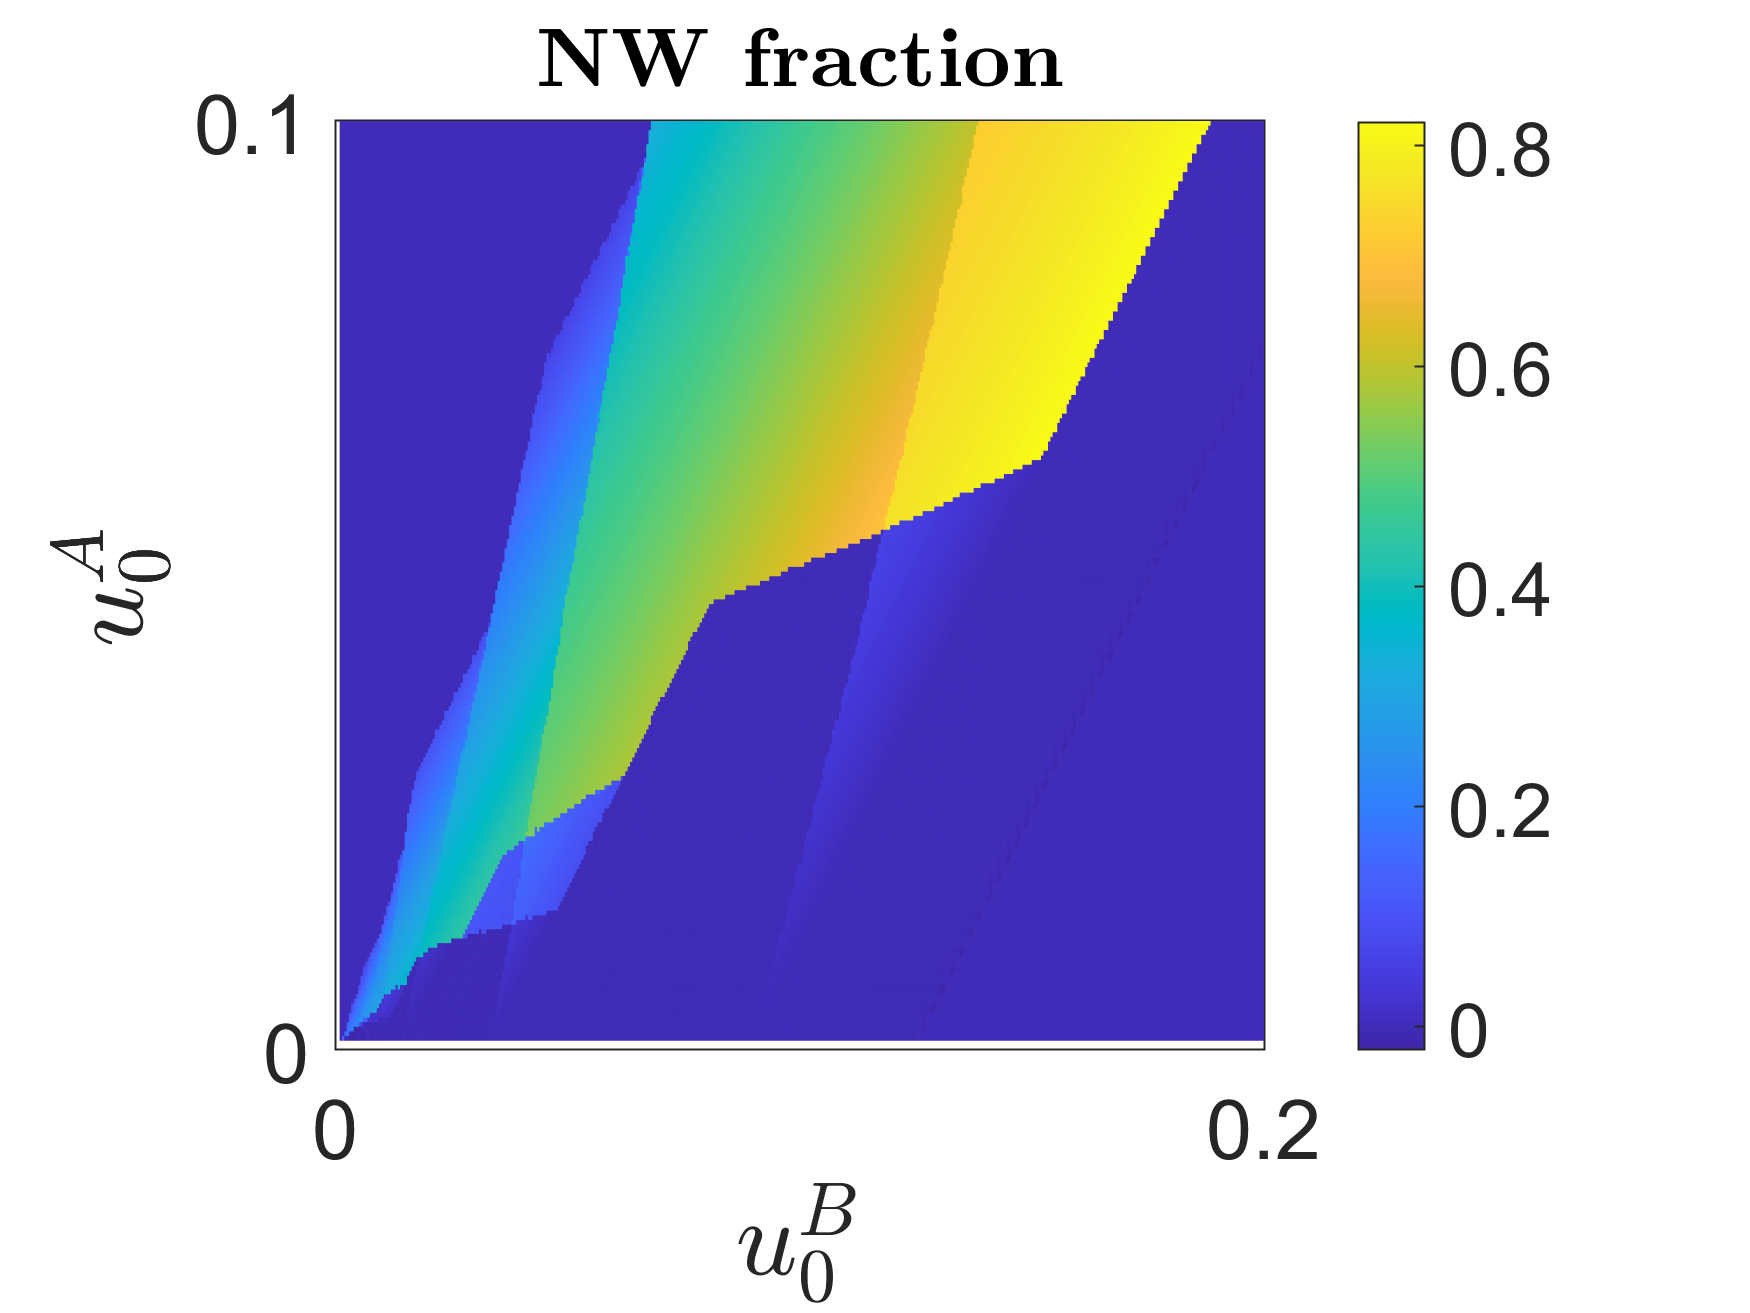
\includegraphics[trim={0cm 0cm 0cm 0cm}, clip,width=0.5\textwidth ]{Images/P5/diferencia.png}
    \caption{The color on the heatmap represents the difference between the informed and ignorant sets fraction. The no winning fraction ($NW$) satisfies the relation $NW = A^{+} - A^{-} = B^{+} - B^{-}$, that is, the difference is the same for both players. Therefore they will fight for being the one informed at the same parameter regions. However for many points the difference is $0$, so being informed or being ignorant results in the same winning set.}
    \label{fig:diferencia}
\end{figure}

It is clear that the second player has advantage in this game if they have the knowledge of the opponent's actions. This way they can counteract any action of the rival. Consequently, the ignorant sets are a subset of the informed ones. Surprisingly, by plotting the difference between the proportion of each player informed and ignorant sets, Fig.~\ref{fig:diferencia}, we can see that there is a major area where the difference is null. This figure is the same as the percentage in which no player guarantees its victory of Fig.~\ref{fig:fraccion}. This is easily demonstrated with the following equations:
\begin{equation}
   \left. \begin{array}{lll}
        &A^{+} + B^{-} = 1 \\
        &A^{-} + B^{+} = 1 \\
        &A^{-} + B^{-} + NW = 1
    \end{array}
    \right\} \Rightarrow NW = A^{+} - A^{-} = B^{+} - B^{-}.
\end{equation}
Here $P^{+}$ represents the proportion of the region $Q$ that is occupied by the informed Player $P$'s winning set while $P^{-}$ the same for the ignorant one. $ NW$ (no winning) is the proportion of blank space when both Player $A$ and Player $B$ are ignorant.

In the case that players could fight for turn order, it is reasonable to assume that there would be a cost associated to being informed. If that is the case, then it may not be worth paying that cost, because the result is the same for a large proportion of cases. However, if one cares to minimize the average control made, being informed is surely beneficial in almost all cases.






\section{Conclusions}

We proposed a novel two-player game of survival in a transient chaotic region. In the game, two players are confronted against each other to control the trajectory of a chaotic dynamical system. The players had opposing goals, each one aiming to get the trajectory to different regions. Through the partial control method we got the set of initial points that guaranteed the victory for each player. Through partial control algorithms we were able to construct winning sets that provided the initial conditions where each player had victory assured. Then, the controlled trajectories are not unique, but at each iteration of the game, the system can be controlled to a range of possible points within the winning sets, giving more flexibility to the controllers.

We applied the game to the logistic map. Here one player aims to stay at the transient chaotic region and the rival wants to drive the trajectory out of there. This system unveils an interesting aspect about the complexity of the dynamical system. Because even when the dynamical system plays against the conservative player and their opponent has greater control capabilities, the player can thrive and achieve their objective.

We also found that the information each player has plays a substantial role in the game. The player that plays first, and therefore knows the action of the rival, will undoubtedly be at an advantage. Therefore, this knowledge was crucial to victory at some cases, but at some other cases, surprisingly, the information was of little use to the informed player.

Finally another interesting result is that when no player knows the action of their rival, regions appear where victory is uncertain. The game is unresolved there and the outcome will depend on the sequence of actions of the players.



\begin{thebibliography}{04}





\bibitem{Yorke}
J. Aguirre, F. d’Ovidio, and M. A. F. Sanjuán,
Controlling chaotic transients: Yorke’s game of survival.
Phys. Rev. E 69:016203
(2004)

\bibitem{DynamicsPartialControl}
Juan Sabuco,1 Miguel A. F. Sanjuan,  1 and James A. Yorke
Dynamics of partial control
Chaos 22:047507
(2012)

\bibitem{PartialControlBeyond}
R.~Cape{\'a}ns, J.~Sabuco, and M.~A.~F. Sanju{\'a}n, 
Beyond partial control: controlling chaotic transients
with the safety function.
Nonlinear Dyn. 107:2903–2910
(2022)


\bibitem{PartialControlFunctions}
R.~Cape{\'a}ns, J.~Sabuco, and M.~A.~F. Sanju{\'a}n, 
A new approach of the partial control method in chaotic systems.
Nonlinear Dyn. 98:873--887
(2019)


\bibitem{PartialControlEscape}
G. Alfaro, R.~Cape{\'a}ns, and M.~A.~F. Sanju{\'a}n, 
Forcing the escape: Partial control of escaping orbits from a
transient chaotic region.
Nonlinear Dyn. 104:1603–1612
(2021) 






\bibitem{Social}
P. Kollock,
Social dilemmas: the anatomy of cooperation.
Annu. Rev. Sociol. 24:183-214
(1998)

\bibitem{EconomyGames}
Y. Xiao, Y. Peng, Q. Lu, and X. Wua,
Chaotic dynamics in nonlinear duopoly Stackelberg game
with heterogeneous players.
Physica A 492:1980--1987
(2018)

\bibitem{GamesComplex}
W. Hu, G. Zang, H. Tian. and Z. Wang,
Chaotic dynamics in asymmetric rock-paper-scissors games.
IEEE Access 7:175614--175621
(2019)


\bibitem{AkiyamaKaneko1}
E. Akiyamaa and K. Kaneko,
Dynamical systems game theory and dynamics of games,
Physica D 147:221--258
(2000)

\bibitem{AkiyamaKaneko2}
E. Akiyamaa and K. Kaneko,
Dynamical systems game theory II
A new approach to the problem of the social dilemma
Physica D 167:36--71
(2002)


\bibitem{GamesControl}
J. R. Marden and J. S. Shamma,
Game Theory and Control.
 Annu. Rev. Control. Robotics Auton. Syst. 1:105--134
(2018)

\bibitem{PartialControlGame}

\end{thebibliography}
\clearemptydoublepage


\chapter{Results and Discussion}
\label{chap:Discussion}



\begin{quotation}
	\vspace{-3cm}
    \begin{flushright}
    \begin{minipage}[t][5cm][b]{0.5\textwidth}
    {\letquote ``Strange game. The only winning move is not to play."}
    
    \bigskip
    
    -{\small  Lawrence Lasker and Walter F. Parkes, WarGames}
    \end{minipage}
    \end{flushright}
    
    \vspace{0.5cm}
\end{quotation}





We have studied one particular evolutionary games, the public goods game, and made alterations to it to examine time-dependent effects that happen in real-life situations. Both examined effects, the oscillations in returns efficacy and a delay in punishment to defectors, hindered cooperation. This is because cooperators need a certain stability to know that their efforts will be worthwhile, and in the case of a delay in punishment, because a rapid punishment is always more susceptible to make the intended effect.

Then we measured complexity in the prisoner's dilemma and the public goods game with the Hamming distance metric. This helped us understand the chaotic pattern formations present when simulating the games spatially, with local interactions. We obtained a measure that may correlate to the Lyapunov time. This measure tells us how much time passes until two configurations are significantly different, and also help us determine the velocity of propagation of changes in configurations of cooperators and defectors.

The studied games can be seen as enormous cellular automata, and therefore, we also analyzed the complexity of the most simple of them to understand the roots of the problem. This are the elementary cellular automata, which can be divided in $4$ classes. 

We obtained an analogue classification to that of Wolfram, but ours focuses on the behavior of the Hamming distance of two close configurations. Class $1$ consist of cellular automata that nullifies the difference between two configurations, while in class $2$ the difference becomes two small and does not change over time. Therefore we can say that the cellular automata in these two classes are stable. On the other hand cellular automata in classes $3$ and $4$ are unstable, with changes rapidly propagating. In class $3$ the Hamming distance behaves chaotically representing the random like patterns that form when plotting the cells' states while in class $4$ the Hamming distance presents transient chaos, which explains the transition between complex patterns to periodical ones but with large periods characteristic of the cellular automata in this class.

By studying the a game of control, we obtained that the key to success can be the correct use of information. The player's that compete in the game are more likely to win the game if they have information about their opponent's moves and of the capabilities of control of both. Is also key to have a precise understanding of the system in which they are playing.


A surprising fact of the game is that the player that has the most challenging goal, to stay inside a transient chaotic region, can sometimes do so even when their control capabilities are inferior to their those of their opponent.

Before studying that game we familiarized with the partial control, by extending the method to the control of escaping trajectories in a quick or in an orderly way. This study was also used when developing the algorithms to solve the competitive game of control. 


Through the interconnected study of game dynamics, complexity and control of chaos, we obtained a broader understanding on how seemingly simple rules can create rich and complex behaviors. Nonetheless, through a precise understanding of the system in play, players can take advantage of the characteristics of the game dynamics and achieve their goals. Therefore the study of game dynamics through tools that come from the complex systems field, provides powerful insight that can be used to solve many real-world problems.

I hope that the breakthroughs and methods collected in the study of this doctoral thesis will help in the investigation of following research in the fields of game theory, complex systems and control.


\clearemptydoublepage


%\chapter{Conclusion}
\label{chap:Conclusion}

\vspace{-2cm}

Here are the main conclusions of this thesis:

\begin{itemize}

\item We have studied two alterations of the public goods game with punishment. We concluded that when investing among peers, unstability in the returns, characterized by an oscillation on the enhancement factor, hinders cooperation. Moreover, the delayed punishment of defectors also makes defectors thrive.


\item We have analyzed the complexity in spacial evolutionary games, even though the system is globally stable since no significant variations of strategy frequencies occur, the local dynamics can be unstable. We obtained a method to measure the complexity of this interactions through the study of the divergence of the Hamming distance of two initially close configurations. Thanks to this tool we arrived at the typical system's time for the two configurations to be far apart.

\item We correctly classified all elementary cellular automata with the Hamming distance measure of diverging configurations. The first two classes are stable to local variations while Class-$3$ and $4$ are unstable. The distance in Class-$3$ behaves chaotically while Class-$4$ presents transitory chaos underlying the phenomenon of edge of chaos.

\item We found a new application to partial control in order to expel trajectories from a transient chaotic region. We have been able to do so with two different approaches. The first one, by accelerating the escape for the trajectories to be expelled in the least time possible. Second, by controlling the escape in order to know how much time passes since we eject control until the trajectory has escaped. Furthermore, we controlled trajectories in multistable systems by setting the time the orbit stays at each region, instead of chaotically shifting to one another.

\item Through the control partial analysis we obtained a useful tool in game theory. We designed a game of control and survival between two confronted players. With the partial control tool helps players can make decisions that gives them the victory at certain initial conditions. We analyzed different cases regarding how much information each player has.

\end{itemize}



\clearemptydoublepage

%%%%%%%%%%%%%%%%%%%%%%%%%%%%%%%%%%%%%%%%%%%%%%%%%%%%%%%%%%%%%%%%%%%%%%% CV Y RESUMEN %%%%%%%%%%%%%%%%%%%%%%%%


%\chapter*{Curriculum Vitae}

\addcontentsline{toc}{chapter}{Curriculum Vitae}  
\markboth{Curriculum Vitae}{}

\hspace{10cm}\includegraphics[width=0.3\textheight]{Images/picture.jpg}



\section*{Publicaciones}

\begin{itemize}

\item
%\bibitem{Alfaro2021}
G. Alfaro, R. Capeáns, and M. A. F. Sanjuán,
Forcing the escape: Partial control of escaping orbits from a
transient chaotic region,
Nonlinear Dyn. \textbf{104}, 1603--1612 (2021).
\url{https://doi.org/10.1007/s11071-021-06331-4}

\item
%\bibitem{Alfaro2022}
G. Alfaro and M. A. F. Sanjuán,
Time-dependent effects hinder cooperation on the public goods game,
Chaos, Solitons Fractals \textbf{160}, 112206 (2022).
\url{https://doi.org/10.48550/arXiv.2501.12188}


\item
%\bibitem{Alfaro2024}
G. Alfaro and M. A. F. Sanjuán,
Hamming distance as a measure of spatial chaos in evolutionary games,
Phys. Rev. E \textbf{109}, 014203 (2024)
\url{10.1103/PhysRevE.109.014203}

\item
G. Alfaro and M. A. F. Sanjuán,
Classification of cellular automata based on the Hamming
distance,
Chaos \textbf{34}, 083129 (2024)
\url{https://doi.org/10.1063/5.0227349}


\item
%\bibitem{PartialControlGame}
G. Alfaro, R. Capeáns, M. A. F. Sanjuán,
Two-player Yorke's game of survival in chaotic transients,
(2025)
\url{https://doi.org/10.48550/arXiv.2501.12188}


\end{itemize}



\section*{Presentaciones en congresos, seminarios y talleres}

\begin{itemize}

\item
\textbf{Seminario:} Seminarios de Investigación del Grupo de Dinámica No Lineal, Teoría del Caos y Sistemas Complejos.

\textbf{Presentación oral}: Dinámica evolutiva en el juego de los bienes públicos.



\textbf{Lugar y fecha}: Universidad Rey Juan Carlos, 21 de abril de 2022.

\item
\textbf{Taller:} Ciencia a la carta.

\textbf{Presentación oral}: Taller de fractales.

\textbf{Lugar y fecha}: Universidad Rey Juan Carlos, 5-7 de abril de 2022.

\item
\textbf{Taller:} XXII Semana de la Ciencia y la Innovación de Madrid.

\textbf{Presentación oral}: Falsifica un Pollock.

\textbf{Lugar y fecha}: Universidad Rey Juan Carlos, 7-20 de noviembre de 2022.

\item
\textbf{Taller:} XXIII Semana de la Ciencia y la Innovación de Madrid.

\textbf{Presentación oral}: Arte y caos.

\textbf{Lugar y fecha}: Universidad Rey Juan Carlos, 6-19 de noviembre de 2023.

\item
\textbf{Seminario:} Seminarios de Investigación del Grupo de Dinámica No Lineal, Teoría del Caos y Sistemas Complejos.

\textbf{Presentación oral}: Distancia de Hamming para medir caos en autómatas celulares elementales y juegos sociales.

\textbf{Lugar y fecha}: Universidad Rey Juan Carlos, 18 de enero de 2024.

\end{itemize}


\section*{Proyectos de investigación}

\begin{itemize}

\item
\textbf{Título}: New challenges in Nonlinear Dynamics of Complex Systems (PID2019-105554GB-I00) 

\textbf{Entidad financiadora}: Agencia Estatal de Investigación

\textbf{Duración}: 01/06/2020 - 31/05/2023

\textbf{Investigador principal}: Miguel Ángel Fernández Sanjuán

\textbf{Tipo de paticipación del doctorando}: Miembro investigador

\textbf{Cuantía de la subvención}: 84.700 euros


\item
\textbf{Título}: Explorando la dinámica no lineal de sistemas complejos. (PID2023-148160NB-I00) 

\textbf{Entidad financiadora}: Agencia Estatal de Investigación

\textbf{Duración}: 01/09/2024 - 31/08/2027

\textbf{Investigador principal}: Miguel Ángel Fernández Sanjuán

\textbf{Tipo de paticipación del doctorando}: Miembro investigador

\textbf{Cuantía de la subvención}: 87.500 euros



\end{itemize}


\section*{Becas}

\begin{itemize}


\item
\textbf{Beca}: C1PREDOC2021 Convocatoria de plazas para contratación de investigadores predoctorales en formación.\\
\textbf{Entidad financiadora}: Universidad Rey Juan Carlos.\\
\textbf{Objeto}: Contratación de personal predoctoral.\\
\textbf{Dotación económica}: 115.200 euros




\end{itemize}

\chapter{Resumen en castellano}
\clearemptydoublepage


\end{document}
